\RequirePackage[l2tabu,orthodox]{nag}

% TODO: decide if one-sided/two-sided
%\documentclass[headsepline,footsepline,footinclude=false,fontsize=11pt,paper=a4,listof=totoc,bibliography=totoc,BCOR=12mm,DIV=12]{scrbook} % two-sided
\documentclass[headsepline,footsepline,footinclude=false,oneside,fontsize=11pt,paper=a4,listof=totoc,bibliography=totoc]{scrbook} % one-sided

% TODO: change citation style in settings
\PassOptionsToPackage{table,svgnames,dvipsnames}{xcolor}

\usepackage[utf8]{inputenc}
\usepackage[T1]{fontenc}
\usepackage[sc]{mathpazo}
\usepackage[ngerman,american]{babel}
\usepackage[autostyle]{csquotes}
\usepackage[%
  backend=biber,
  url=false,
  style=numeric,
  maxnames=4,
  minnames=3,
  maxbibnames=99,
  giveninits,
  uniquename=init]{biblatex} % TODO: adapt citation style
\usepackage{graphicx}
\usepackage{scrhack} % necessary for listings package
\usepackage{listings}
\usepackage{lstautogobble}
\usepackage{tikz}
\usepackage{pgfplots}
\usepackage{pgfplotstable}
\usepackage{booktabs}
\usepackage[final]{microtype}
\usepackage{caption}
\usepackage[hidelinks]{hyperref} % hidelinks removes colored boxes around references and links



\bibliography{bibliography}

\AtBeginBibliography{\sloppy}
\pretocmd{\bibsetup}{\hyphenpenalty=5000 \tolerance=1000 \emergencystretch=3em}{}{}
\DeclareFieldFormat{title}{\parbox[t]{\dimexpr\linewidth-1em}{\textbf{#1}}}
\pretocmd{\bibsetup}{\sloppy\emergencystretch=3em}{}{}



% \DeclareFieldFormat{title}{\textbf{\emph{\nohyphens{#1}}}} % Allow hyphenation in titles
% \DeclareFieldFormat{journaltitle}{\textit{\nohyphens{#1}}} % Allow hyphenation in journals



\setkomafont{disposition}{\normalfont\bfseries} % use serif font for headings
\linespread{1.05} % adjust line spread for mathpazo font

% Add table of contents to PDF bookmarks
\BeforeTOCHead[toc]{{\cleardoublepage\pdfbookmark[0]{\contentsname}{toc}}}

% Define TUM corporate design colors
% Taken from http://portal.mytum.de/corporatedesign/index_print/vorlagen/index_farben
\definecolor{TUMBlue}{HTML}{0065BD}
\definecolor{TUMSecondaryBlue}{HTML}{005293}
\definecolor{TUMSecondaryBlue2}{HTML}{003359}
\definecolor{TUMBlack}{HTML}{000000}
\definecolor{TUMWhite}{HTML}{FFFFFF}
\definecolor{TUMDarkGray}{HTML}{333333}
\definecolor{TUMGray}{HTML}{808080}
\definecolor{TUMLightGray}{HTML}{CCCCC6}
\definecolor{TUMAccentGray}{HTML}{DAD7CB}
\definecolor{TUMAccentOrange}{HTML}{E37222}
\definecolor{TUMAccentGreen}{HTML}{A2AD00}
\definecolor{TUMAccentLightBlue}{HTML}{98C6EA}
\definecolor{TUMAccentBlue}{HTML}{64A0C8}

% Settings for pgfplots
\pgfplotsset{compat=newest}
\pgfplotsset{
  % For available color names, see http://www.latextemplates.com/svgnames-colors
  cycle list={TUMBlue\\TUMAccentOrange\\TUMAccentGreen\\TUMSecondaryBlue2\\TUMDarkGray\\},
}

% Settings for lstlistings
\lstset{%
  basicstyle=\ttfamily,
  columns=fullflexible,
  autogobble,
  keywordstyle=\bfseries\color{TUMBlue},
  stringstyle=\color{TUMAccentGreen}
}


% TODO: change thesis information
\newcommand*{\getUniversity}{Techncal University of Munich}
\newcommand*{\getFaculty}{ TUM School of Computation, Information and Technology }
\newcommand*{\getTitle}{Special Handling of Fast Particles in AutoPas to Reduce Rebuild Time}
\newcommand*{\getAuthor}{Xhulia Jasimi}
\newcommand*{\getDoctype}{Bachelor's Thesis in Informatics}
\newcommand*{\getSupervisor}{Univ.-Prof. Dr. Hans-Joachim Bungartz}
\newcommand*{\getAdvisor}{Samuel James Newcome, M.Sc.}
\newcommand*{\getSubmissionDate}{17.02.2025}
\newcommand*{\getSubmissionLocation}{Munich}

\usepackage{lipsum}
\usepackage{ulem}
\usepackage{listings}
\usepackage{xcolor}
\usepackage{multicol}
\usepackage{graphicx}
\usepackage{caption}
\usepackage{subcaption} % For subfigures
\usepackage{float}  
\usepackage[export]{adjustbox} 
\usepackage{wrapfig}  % For wrapping figures around text
\usepackage{array} 
\usepackage{tabularx}

\definecolor{commentgray}{rgb}{0.5, 0.5, 0.5}
\definecolor{keywordred}{rgb}{0.9, 0.3, 0.3}
\definecolor{keyorange}{rgb}{0.9, 0.6, 0.3}

\lstdefinestyle{cppstyle}{
    language=C++,               % Set the language to C++
    basicstyle=\ttfamily\small,  % Use typewriter font (monospaced)
    keywordstyle=\color{blue},   % Keywords in blue
    commentstyle=\color{green},  % Comments in green
    stringstyle=\color{red},     % Strings in red
    numbers=left,                % Line numbers on the left
    numberstyle=\tiny\color{gray},  % Small, gray line numbers
    frame=single,                % Frame around the code
    breaklines=true,             % Automatically break long lines
    tabsize=4,                   % Set the tab size to 4 spaces
    captionpos=b                 % Caption below the code
}

\lstdefinestyle{mypython}{
    language=Python,
    basicstyle=\ttfamily\small,
    keywordstyle=\color{blue},
    stringstyle=\color{green},
    commentstyle=\color{gray},
    numbers=left,
    numberstyle=\tiny\color{gray},
    stepnumber=1,
    breaklines=true,
    showstringspaces=false,
    frame=single,
}
% \bibliographystyle{plain}  % Use IEEE, apalike, etc., as needed
% \bibliography{bibliography} 

\begin{document}

% Set page numbering to avoid "destination with the same identifier has been already used" warning for cover page.
% (see https://en.wikibooks.org/wiki/LaTeX/Hyperlinks#Problems_with_Links_and_Pages).
\pagenumbering{alph}
\input{pages/cover}

\frontmatter{}

\begin{titlepage}
  \centering

  \IfFileExists{logos/tum.pdf}{%
    \includegraphics[height=20mm]{logos/tum.pdf}
  }{%
    \vspace*{20mm}
  }

  \vspace{5mm}
  {\huge\MakeUppercase{\getFaculty{}}}\\

  \vspace{5mm}
  {\large\MakeUppercase{\getUniversity{}}}\\

  \vspace{20mm}
  {\Large \getDoctype{}}

  \vspace{15mm}
  {\huge\bfseries \getTitle{} \par}

  % \vspace{10mm}
  % {\huge\bfseries \foreignlanguage{ngerman}{\getTitleGer{}} \par}

  \vspace{15mm}
  \begin{tabular}{l l}
    Author:          & \getAuthor{} \\
    Supervisor:      & \getSupervisor{} \\
    Advisor:         & \getAdvisor{} \\
    Submission Date: & \getSubmissionDate{} \\
  \end{tabular}

  \IfFileExists{logos/faculty.pdf}{%
    \vfill{}
    \includegraphics[height=20mm]{logos/faculty.pdf}
  }{}
\end{titlepage}

\input{pages/disclaimer}
\addcontentsline{toc}{chapter}{Acknowledgments}
\thispagestyle{empty}

\vspace*{20mm}

\begin{center}
{\usekomafont{section} Acknowledgments}
\end{center}

\vspace{10mm}


I would like to express my sincere gratitude to my advisor, Samuel James Newcome, for his continuous support throughout this thesis. His guidance during our meetings and his willingness to answer every question—no matter how many emails I sent—were invaluable.  

I would also like to thank the Chair of Scientific Computing and Prof. Dr. Hans-Joachim Bungartz for providing the opportunity and resources to conduct this research.  

A heartfelt thank you to my family for always supporting me in every journey I embark on. Finally, I am deeply grateful to my friends, who patiently listened to me talk about my thesis for four months straight.  


\cleardoublepage{}

\chapter{\abstractname}

Simulating particle interactions is a fundamental challenge in computational physics, molecular dynamics, and engineering applications. Efficiently managing these simulations is particularly important in large-scale systems, where millions of particles interact over extended periods of time. A key aspect of these simulations is the identification of particles which are eligible for pairwise force calculations. In algorithms like Verlet Lists, these particles are stored in neighbor lists, which are periodically rebuilt to maintain accuracy.

This thesis investigates the Fast-Particle-Buffer mechanism as an alternative approach to optimize the neighbor list rebuild process in AutoPas, a performance-optimized C++ library for short-range particle simulations. Instead of triggering a full rebuild whenever fast-moving particles exceed a predefined threshold, these particles are temporarily stored in a buffer, allowing the neighbor lists to be used longer before rebuilding. 

Through various test scenarios, this approach is evaluated in terms of computational efficiency and its impact on overall simulation performance. The findings suggest that while the Fast-Particle-Buffer can reduce neighbor list rebuild costs, its effectiveness depends on the simulation's characteristics. 


\microtypesetup{protrusion=false}
\tableofcontents{}
\microtypesetup{protrusion=true}

\mainmatter{}

\chapter{Introduction}\label{chapter:introduction}


% Simulating particle interactions is a fundamental problem in computational physics, molecular dynamics, and engineering applications. Efficiently handling these simulations is crucial, particularly in large-scale systems where millions of particles interact over extended time periods. These simulations can be very computationally demanding, making runtime optimization a critical objective to improve performance and scalability. \parencite{aktulga2012parallel}

Simulating particle interactions plays a crucial role in computational physics, molecular dynamics, and engineering applications. In large-scale systems, where millions of particles interact over extended time periods, these simulations require significant computational resources. As a result, optimizing runtime is essential to improve efficiency, performance, and scalability. \parencite{aktulga2012parallel}


AutoPas is an auto-tuning C++ library designed to optimize short-range particle simulations by selecting the most efficient algorithm for a given simulation. The library implements various algorithms. However, since each simulation is unique, there is no single best algorithm that performs optimally in all cases. To address this, AutoPas uses auto-tuning, which dynamically selects the most efficient combination of internal algorithms during run-time \parencite{seckler2021autopas}.

One of the internal algorithms provided by AutoPas is Verlet Lists. A key challenge in Verlet Lists is the computational overhead caused by frequent neighbor list rebuilds. As particles move dynamically within the simulation domain, neighbor lists—which store information about neighboring particles within a defined search region—become outdated and must be recomputed periodically. This rebuilding is computationally expensive, impacting overall simulation performance.

This thesis investigates an alternative approach: the Fast-Particle-Buffer mechanism. Instead of rebuilding neighbor lists whenever a fast-moving particle enters the search region, the buffer temporarily stores these particles and avoids neighbor lists rebuilding. The goal is to analyze whether this strategy can reduce computational overhead and improve overall simulation performance.

% To evaluate this approach, various simulation scenarios were tested, each chosen to reflect different particle behaviors and interaction dynamics. The experiments were conducted using AutoPas, and the results provide insights into when and where the Fast-Particle-Buffer mechanism offers advantages.

The structure of this thesis is as follows: Chapter 2 provides a theoretical background on molecular dynamics and intorduces AutoPas. Chapter 3 presents related projects, while Chapter 4 details the implementation of the Fast-Particle-Buffer mechanism. Chapter 5 presents experimental results, analyzing the efficiency of the proposed approaches across various scenarios. Finally, Chapter 6 discusses potential future optimizations, followed by Chapter 7, which summarizes the key findings and conclusions of this work.



\chapter{Background}

\section{Molecular Dynamics (MD) Simulations}

Molecular dynamics (MD) is a computational method used to analyze the interactions and movements of atoms and molecules. It offers better understanding of dynamic processes at atomic scale, such as diffusion, chemical reactions, and phase changes, making it an essential tool in physics, bioinformatics, molecular biology, materials science, and more. MD simulations are widely used to study protein folding, predict material properties, discover drugs, and analyze system behavior under various conditions \parencite{kukol2008molecular} \parencite{aktulga2012parallel}
% [\textbf{existingTuning second reference, Downloads/978-1-59745-177-2.pdf}].

MD simulations begin with an initial configuration of particles, with specified positions and velocities. Forces acting on each particle are calculated using a force field, which defines the potential energy of the system. These forces are then translated into velocities and movements. Over discrete time steps, the positions and velocities of particles are updated, providing a dynamic view of the system's evolution.

% MD operates within the framework of classical mechanics, treating particles as point masses and neglecting quantum mechanical effects unless explicitly modeled using hybrid approaches. While this classical approach is suitable for many applications, phenomena such as chemical bond breaking or electronic transitions require reactive force fields or quantum mechanical methods [\textbf{existingTuning, parallelcomputing}].

\subsection{Computational Challenges and Optimizations}

While MD is a powerful tool, it is computationally expensive, requiring a significant amount of resources to deliver accurate and reliable results. The main challenges include handling large system sizes, modeling long simulation times, and accurately capturing diverse interactions.

\subsubsection{Short-Range Simulations} \label{sec:shortrange}

To balance computational efficiency and accuracy of results, approximations are commonly introduced. While the distance between two particles increases, the pairwise forces between the two start converging to zero, and can therefore be ignored. For these types of potentials, called short-range potentials, a cutoff radius (\(r_c\)) is introduced. This approximation assumes that interactions beyond \(r_c\) are negligible and can be ignored. By doing so, the computational complexity is reduced from \(O(N^2)\) to \(O(N)\), where \(N\) is the number of particles. \parencite{gratl2022n}

% [\textbf{Gratl 2022.pdf}] 
% However, long-range potentials, while computable using advanced techniques, are not natively supported in AutoPas and are outside the scope of this discussion.

\subsubsection{Lennard-Jones Potential (LJ)}

The Lennard-Jones 12-6 potential is a widely used function in molecular dynamics simulations to model interactions between particles, such as atoms or molecules. It describes the balance between short-range repulsion and long-range attraction forces. This balance is given by:

\[
V(r) = 4\epsilon \left[ \left(\frac{\sigma}{r}\right)^{12} - \left(\frac{\sigma}{r}\right)^{6} \right],
\]

where \(r\) is the distance between two particles, \(\epsilon\) is the depth of the potential well, representing the strength of attraction, and \(\sigma\) is the distance at which the potential changes sign. \parencite{wang2020lennard}

The first term, \((\sigma/r)^{12}\), models the steep repulsive forces that dominate at very short distances, while the second term, \((\sigma/r)^{6}\), represents the weaker attractive van der Waals forces. The potential reaches its minimum value at \(r = 2^{1/6} \sigma\), which corresponds to the equilibrium distance between particles.

The Lennard-Jones potential is particularly suited for short-range interactions due to its rapid convergence to zero as \(r\) increases. \parencite{jones1924determination}

% [\textbf{jones1924determination, wang2020lennard, inproceedings for picture}].

\begin{figure}[ht]
\centering
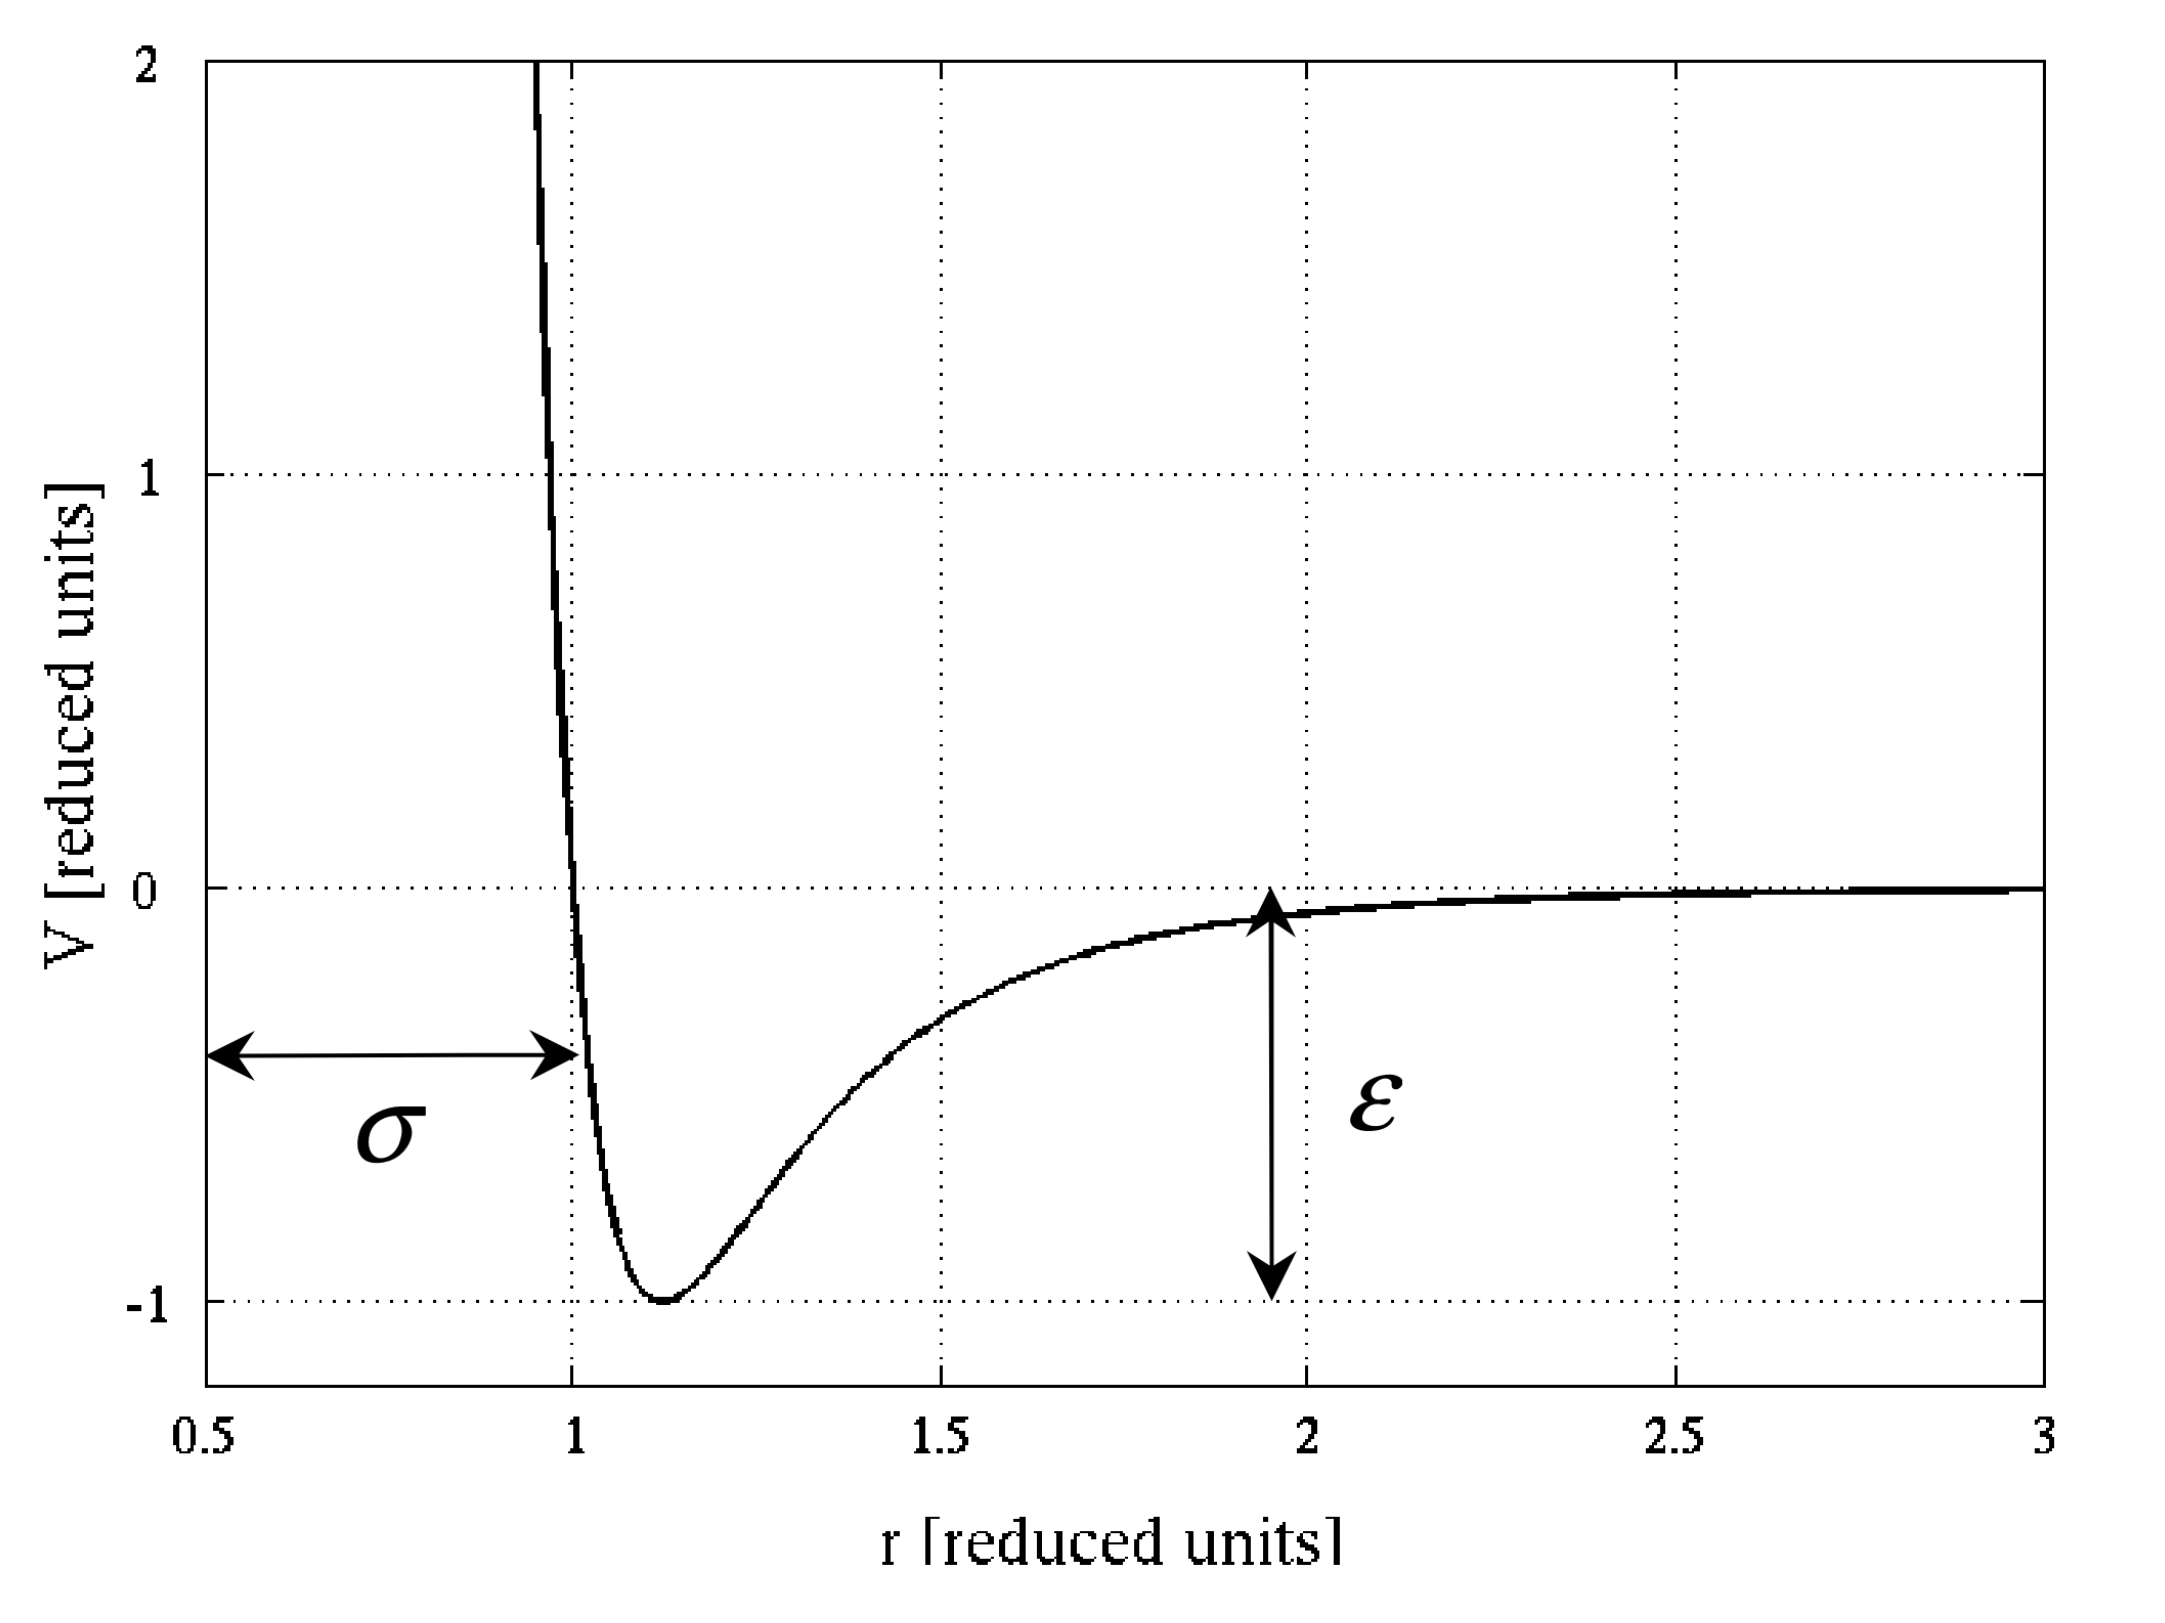
\includegraphics[%scale=1
                 width=0.5\linewidth, valign=t]{imgs/lj.png}
\caption{Lennard-Jones Potential \parencite{inproceedings}}
\label{lj}
\end{figure}



\subsubsection{Newton's Third Law}

An essential optimization in MD simulations is the application of Newton's third law, which states that every action has an equal and opposite reaction; or, the mutual actions of two bodies upon each other are always equal, and directed to contrary parts \parencite{frautschi1986mechanical}. 
 In particle simulations, this means the force that particle \(p_1\) exerts on \(p_2\) is equal and opposite to the force \(p_2\) exerts on \(p_1\). Using this symmetry halves the number of force calculations, significantly improving computational efficiency. In AutoPas, this optimization is implemented as the Newton3-optimization \parencite{gratl2022n}.


\section{AutoPas Software}

AutoPas is a C++ library specifically designed to optimize short-range particle simulations through dynamic algorithm selection. It acts as a black box, where users provide the specifications while the library handles the choice of the best suitable algorithm through auto-tuning. By periodically evaluating various algorithms, AutoPas ensures that the most efficient configuration is applied as simulation conditions change. The library includes example applications, such as the md-flexible framework, which will be used in the course of this thesis \parencite{gratl2019autopas}.


\subsection{Data layouts}

AutoPas supports two primary data layouts for storing particle information in memory: Array of Structures (AoS) and Structure of Arrays (SoA). In the AoS layout, each particle is represented as an object containing all its properties, such as position and force, stored together in memory. This arrangement allows for efficient cache utilization when accessing individual particles, but can limit vectorization efficiency. On the other hand, the SoA layout separates particle properties into individual arrays, with each array containing data for all particles, leading to better vectorization by aligning data contiguously in memory. However, this layout may lead to less efficient cache usage when accessing properties of a single particle \parencite{gratl2019autopas}.

\subsection{Neighbor identification algorithms} \label{sec:neighbor_iden_algs}

During auto-tuning AutoPas has to decide how to manage and store the particles of the simulation, and most importantly how to identify the neighboring particles to efficiently compute the pairwise forces. As shown in section \ref{sec:shortrange}, for each particle, the particles within the cut-off radius should be found, and the rest will be ignored. This process is repeated for every single particle in the container, and choosing the right Neighbor identification algorithm, is crucial when it comes to performance. Below, the four algorithms used in AutoPas are presented. These algorithms are implemented as containers in AutoPas, managing neighbor identification and the overall particle organization, including the selection of the data layout. 

\subsubsection{Direct Sum}

The straightforward, and thus naive, approach, is to calculate the distances from one particle to all other particles without utilizing any additional data structures. Instead, all particles are stored in a single cell, and for each particle, distances to all other particles are evaluated to determine whether they fall within the cutoff radius. Forces are only computed for pairs of particles within this radius. As illustrated in \hyperref[fig:directsum]{Figure \ref*{fig:directsum}}, the red particle represents the current particle, for which forces are being calculated, the red circle denotes the cutoff radius, and the arrows depict the interactions between the current particle and the others.

This method, while eliminating the complexity and overhead associated with bigger data structures, is computationally inefficient. The calculation of pairwise forces results in a time complexity of \(O(n^2)\), where \(n\) is the number of particles \parencite{gratl2022n}. Although simple, this approach is only practical for simulations with a very small number of particles.


\subsubsection{Linked Cells}

This approach extends the Direct Sum method by dividing the simulation domain into cells, with each cell containing the particles within its boundaries. The cell dimensions are set to at least the cutoff radius (\(r_c\)). This ensures that short-range interactions are computed only between particles in the current cell and its eight neighboring cells, as depicted with blue in \hyperref[fig:linkedcells]{Figure \ref*{fig:linkedcells}}.

Because the cell size matches the cutoff radius, particles outside these neighboring cells are guaranteed to lie beyond the interaction range and can be excluded from force calculations. For homogeneous particle distributions, this reduces the computational complexity from \(O(n^2)\) to \(O(n)\) \parencite{knapek2007numerical}. Furthermore, Linked Cells improve cache efficiency by storing particles within the same cell contiguously in memory. 

Nonetheless, there is still computational overhead, as around 84.5\% of the particles in the search region are outside the cutoff radius, leading to redundant distance calculations. The probability of finding a pair of particles within the cutoff radius in a 3D simulation, is approximately 15.5\% and can be estimated using the following equation \parencite{gratl2019autopas}:

\[
\frac{\textit{Cutoff volume}}{\textit{Search volume}_{LC}} =
\frac{\frac{4}{3} \pi r_c^3}{(3r_c)^3}
\]

\subsubsection{Verlet Lists} \label{sec:verletlists}

The idea behind Verlet Lists is to precompute and store neighbor lists for each particle. This allows the AutoPas to efficiently track all nearby particles within a particle's cutoff radius, making pairwise interaction calculations faster by reducing the number of distance checks needed in each iteration.

Since particles move during the simulation, these lists eventually become outdated and need to be rebuilt whenever a new particle enters or leaves the cutoff region. To reduce how often these lists need to be rebuilt, an additional safety margin is introduced, known as the Verlet skin factor \(s\). The cutoff radius \(r_c\) is scaled by this factor, expanding the search radius to \(r_c \cdot s\), as shown with yellow in Figure~\ref{fig:verletlists}. This extended region allows the neighbor lists to remain valid for multiple iterations, reducing the frequency of rebuilds.

With this approach, the probability of finding a particle in the cutoff region in a 3D simulation domain is given by \parencite{gratl2019autopas}:

\[
\frac{\textit{Cutoff volume}}{\textit{Search volume}_{VL}} =
\frac{\frac{4}{3} \pi r_c^3}{\frac{4}{3} \pi (r_c \cdot s)^3} =
\frac{1}{s^3}.
\]


Selecting an appropriate skin factor is crucial, as it affects both the number of unnecessary calculations and how often the neighbor lists are rebuilt. For instance, a skin factor of 1.2 reduces the number of unnecessary distance calculations by half compared to Linked Cells.

Throughout the simulation, as particles move, two cases arise:
\begin{itemize}
    \item If a particle moves away from another, it may remain in the neighbor list longer than necessary, increasing storage costs and unnecessary force calculations.
    \item If a particle moves closer to another, it may enter its cutoff radius but not be included in the neighbor list, leading to incorrect force calculations.
\end{itemize}

To avoid these issues, AutoPas uses a fixed rebuild frequency parameter, ensuring that all neighbor lists are rebuilt every \(N\) iterations to keep them compact and accurate. 


On top of that, when using dynamic containers as described in \parencite{gall2023exploration}, the maximum particle displacement per iteration is used as a metric of when to rebuild. In this case the displacement of each particle from its last rebuild position is tracked in every iteration. This displacement is then compared to a threshold, which is chosen as half of the Verlet skin size \parencite{thompson2022lammps}. If at least one particle exceeds this threshold, it could have entered the cutoff region of another particle, and therefore the neighbor lists are rebuilt.


To improve efficiency, AutoPas builds the Verlet Lists algorithm on top of Linked Cells. Therefore, the neighbor lists are constructed by assessing only particles in neighboring cells. This allows the computational complexity to be reduced from \(O(N^2)\) (brute-force search) to \(O(N)\) \parencite{yao2004improved}. 

Verlet Lists are particularly effective for systems with high particle densities. However, their lack of spatial locality can lead to inefficient memory access, resulting in poor cache performance and reduced vectorization efficiency \parencite{gratl2022n}.


\subsubsection{Verlet Cluster Lists}

Verlet Cluster Lists are built upon regular Verlet Lists by grouping particles into clusters rather than maintaining individual neighbor lists for each particle Figure~\ref{fig:verletclusters}. This approach reduces memory overhead, as a single neighbor list is created for each cluster instead of one for every particle. The algorithm uses the observation that neighboring particles often share similar neighbor lists, allowing $M$ particles to be combined into a cluster. When two clusters are close, all interactions between the particles within these clusters are calculated. This optimization decreases the number of neighbor lists by a factor of $\frac{1}{M}$ \parencite{gratl2022n}, and enhances computational efficiency by enabling better vectorization. However, the increased search radius, can lead to additional distance calculations. Despite this, Verlet Cluster Lists are well-suited for large systems with high particle densities.

\begin{figure}[h!]
    \centering
    % First Figure
    \begin{subfigure}{0.22\textwidth}
        \centering
        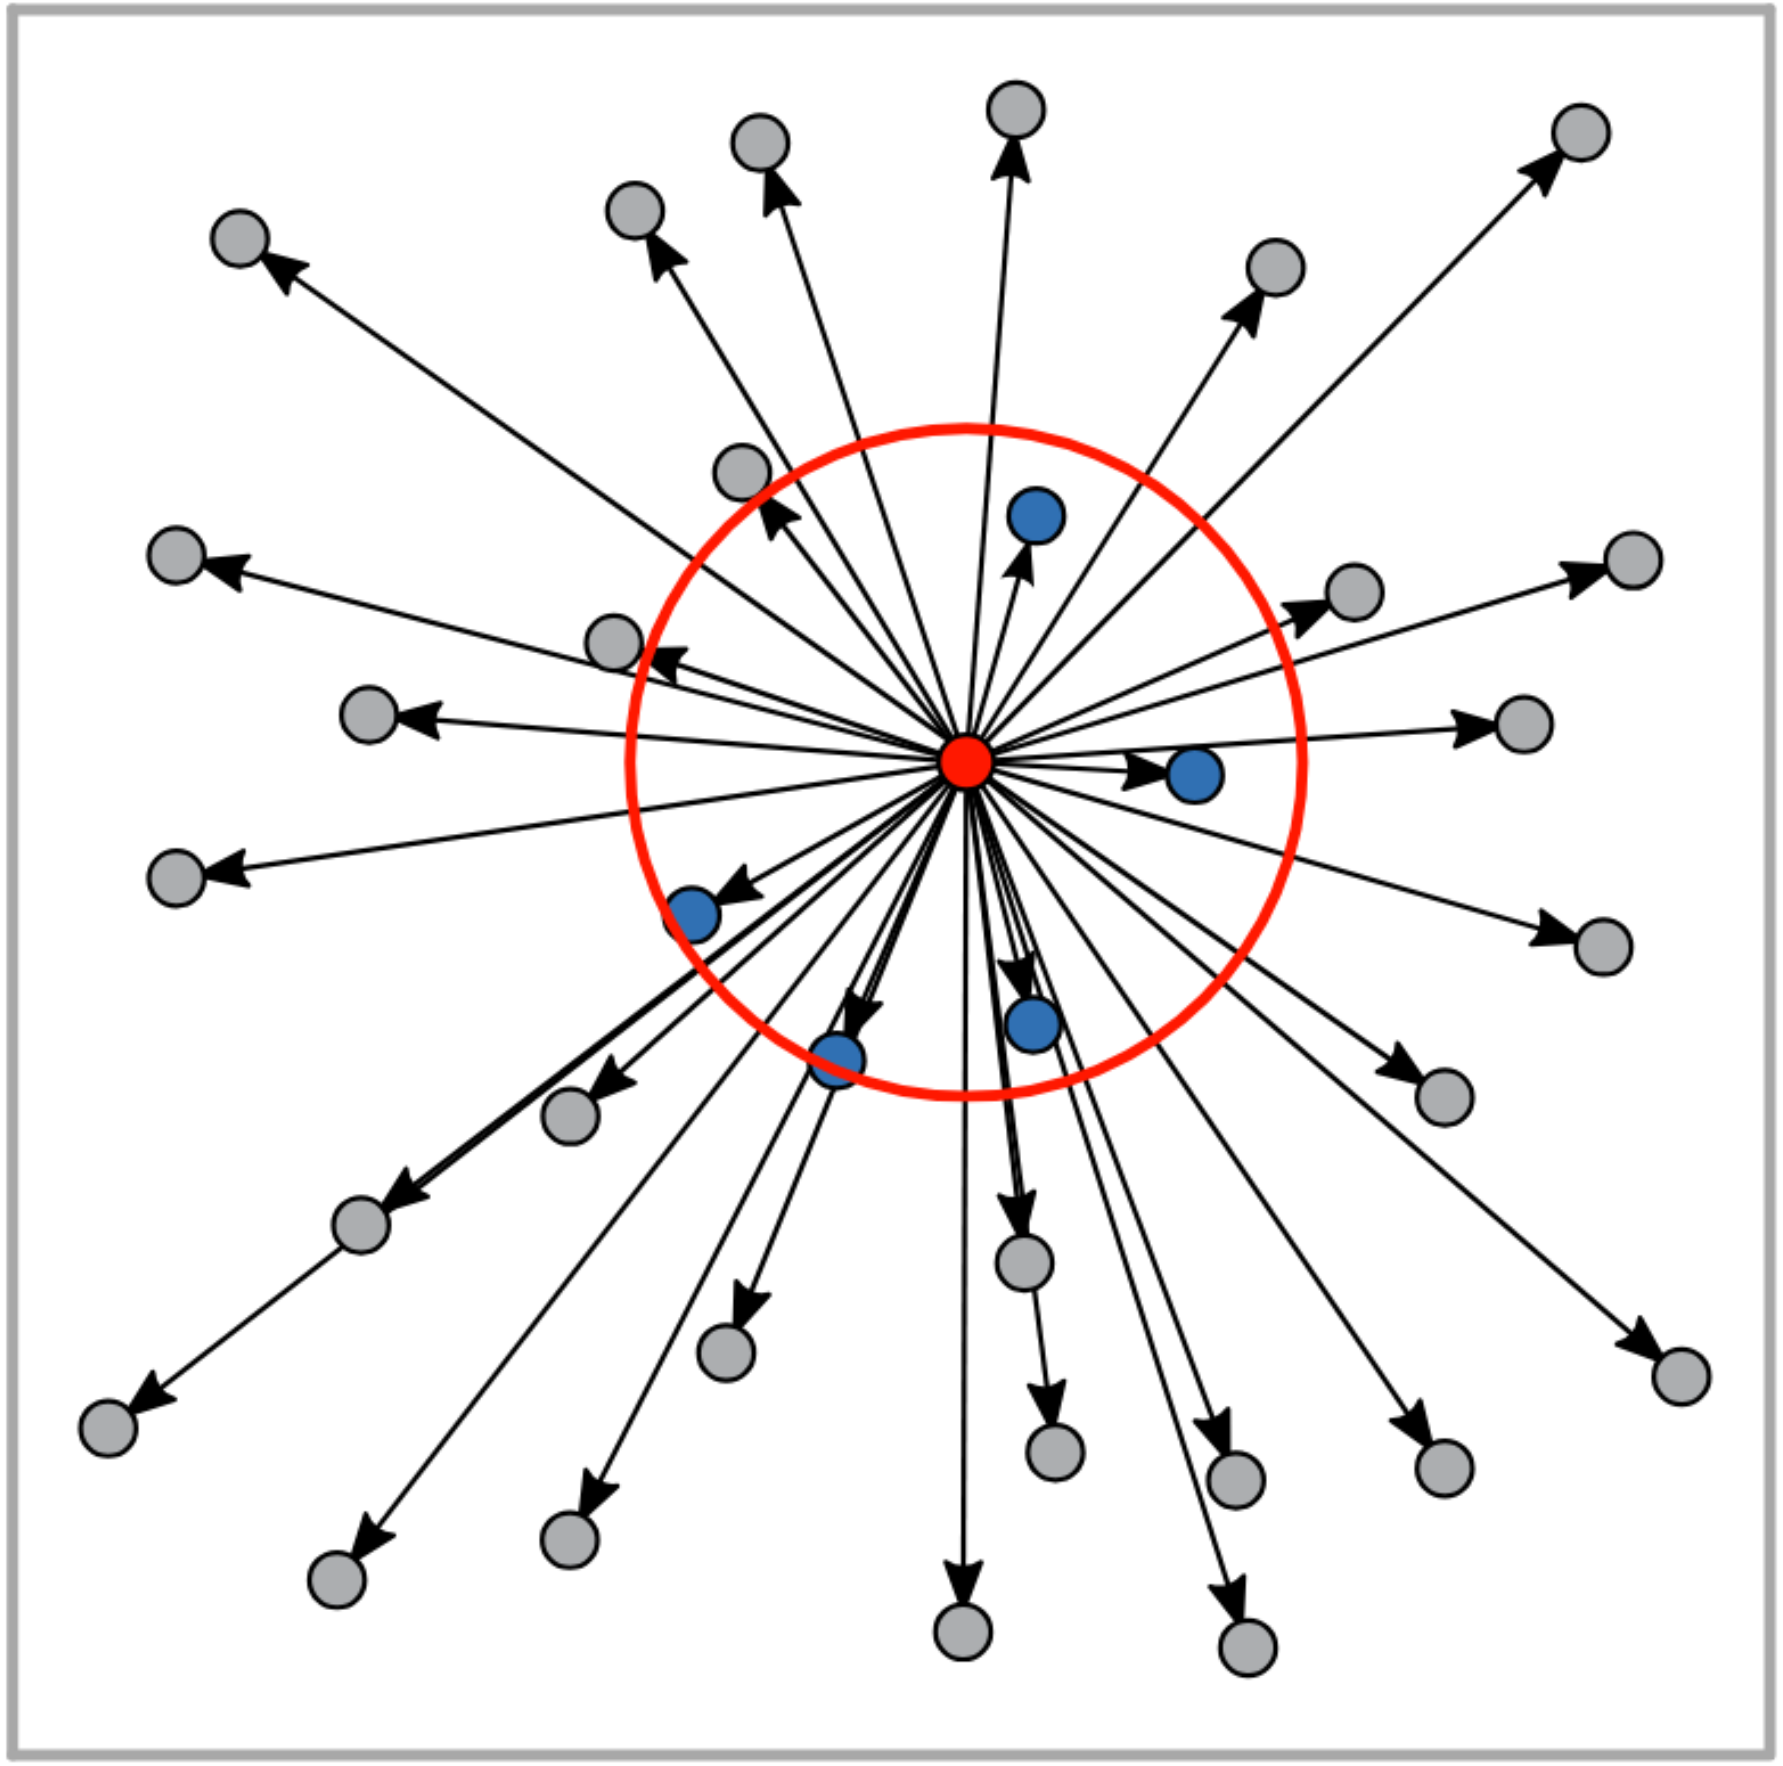
\includegraphics[width=\linewidth]{imgs/directsum.png}
        \caption{\scriptsize Direct Sum}
        \label{fig:directsum}
    \end{subfigure}
    \hfill
    % Second Figure
    \begin{subfigure}{0.22\textwidth}
        \centering
        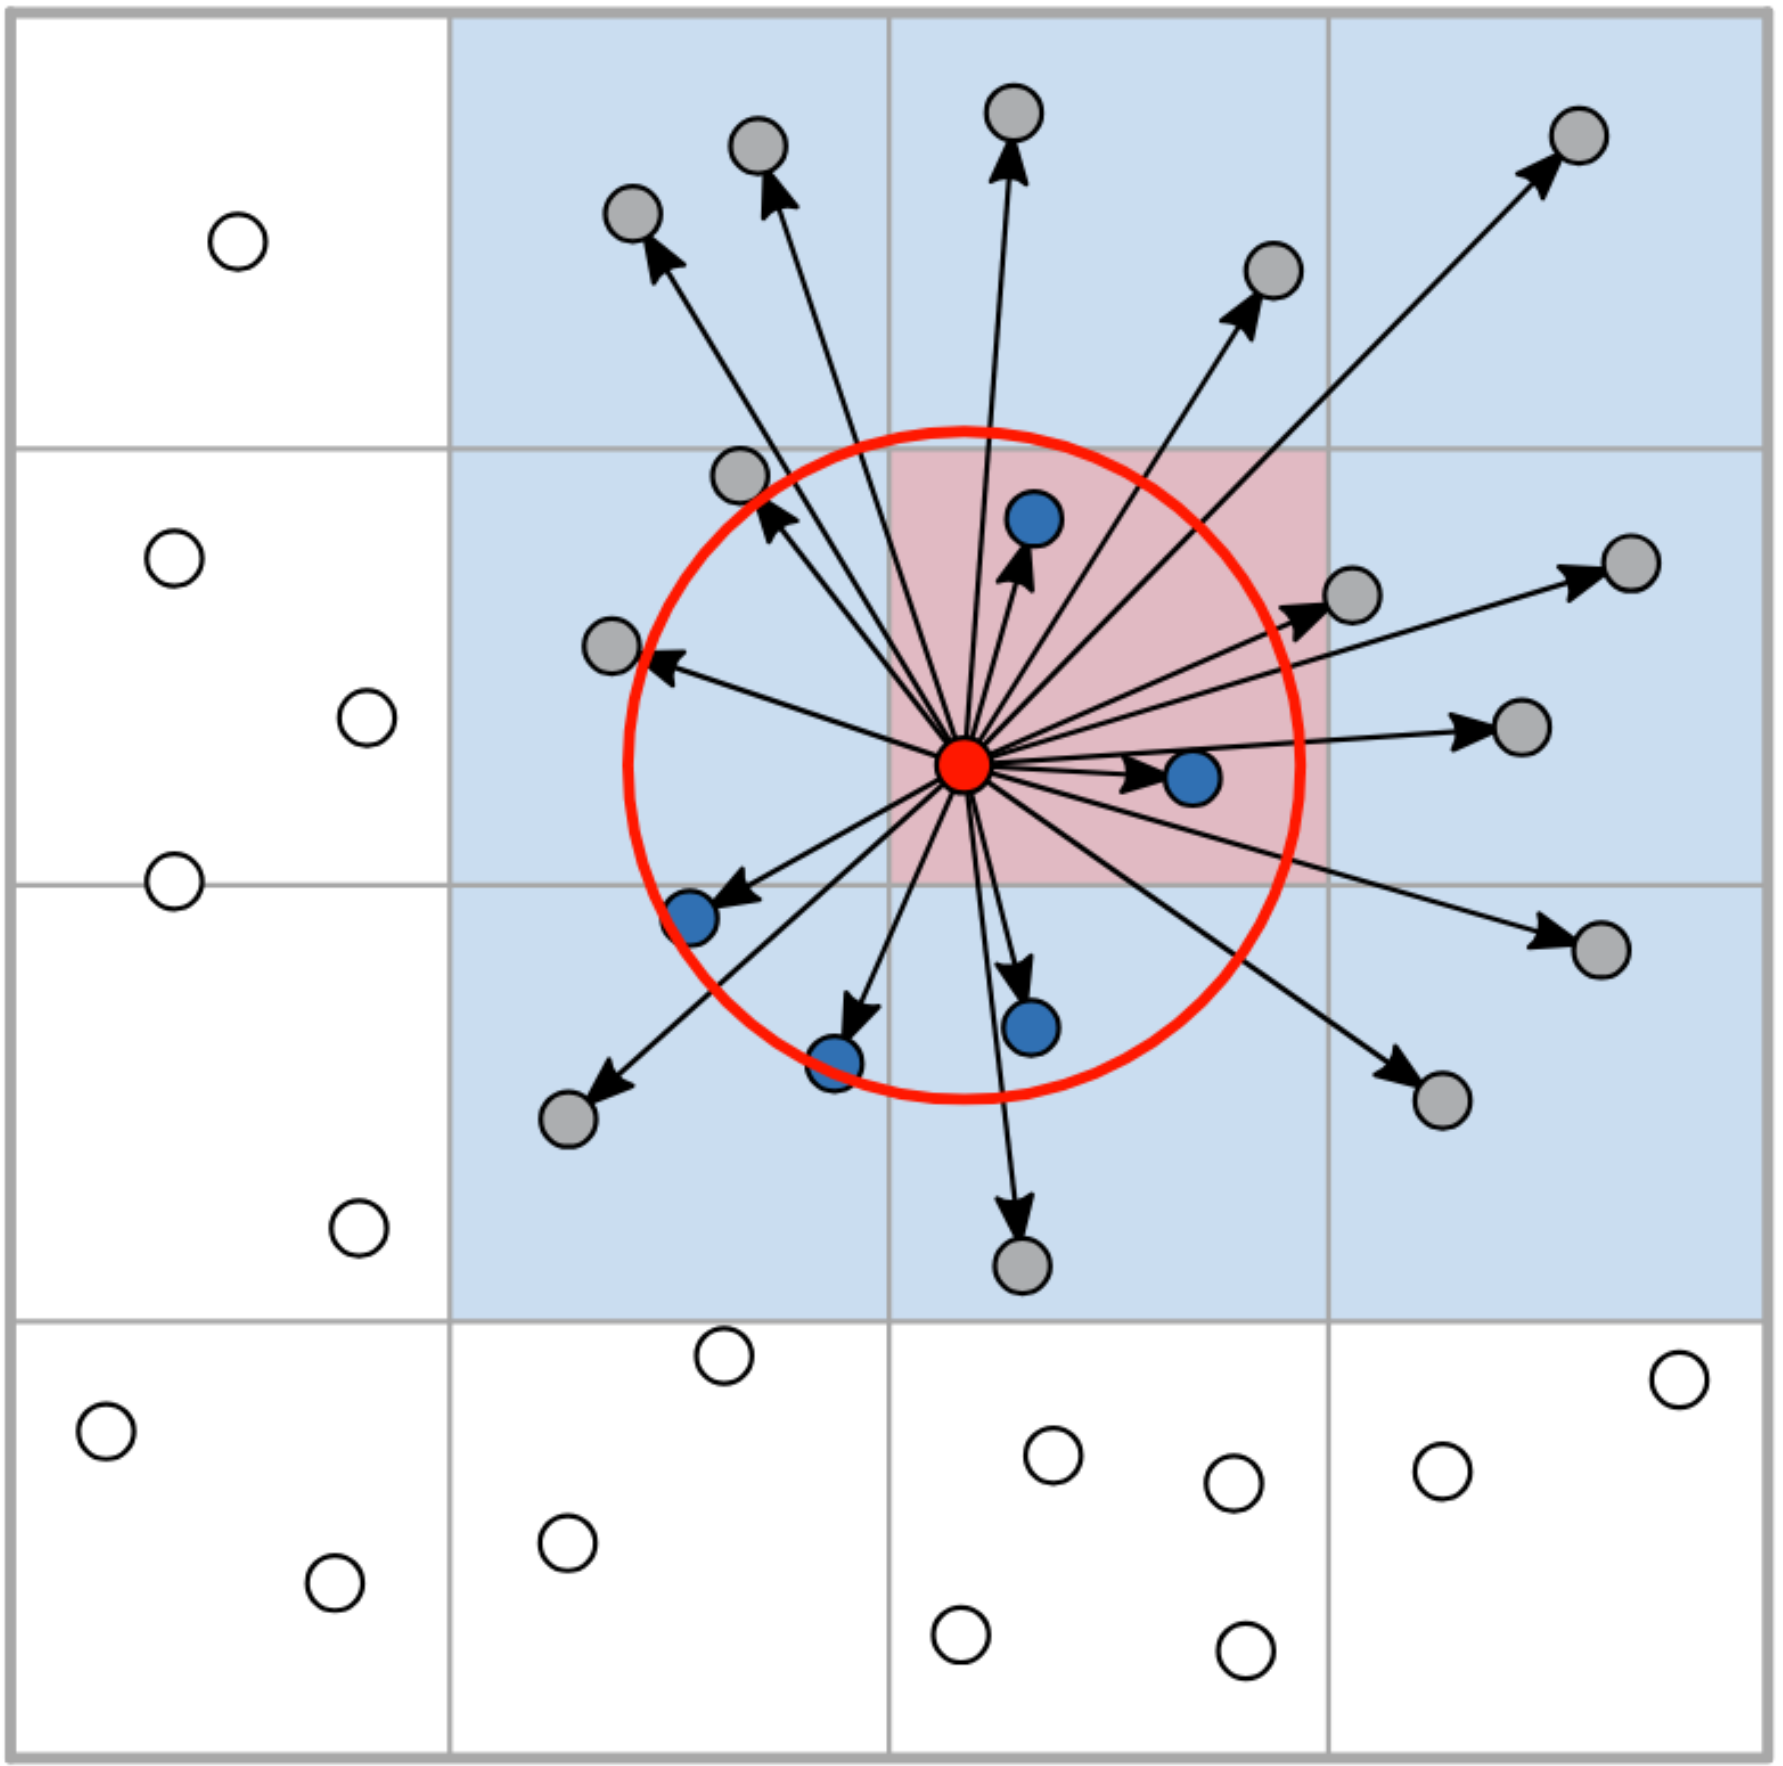
\includegraphics[width=\linewidth]{imgs/linkedcells.png}
        \caption{\scriptsize Linked Cells}
        \label{fig:linkedcells}
    \end{subfigure}
    \hfill
    % Third Figure
    \begin{subfigure}{0.22\textwidth}
        \centering
        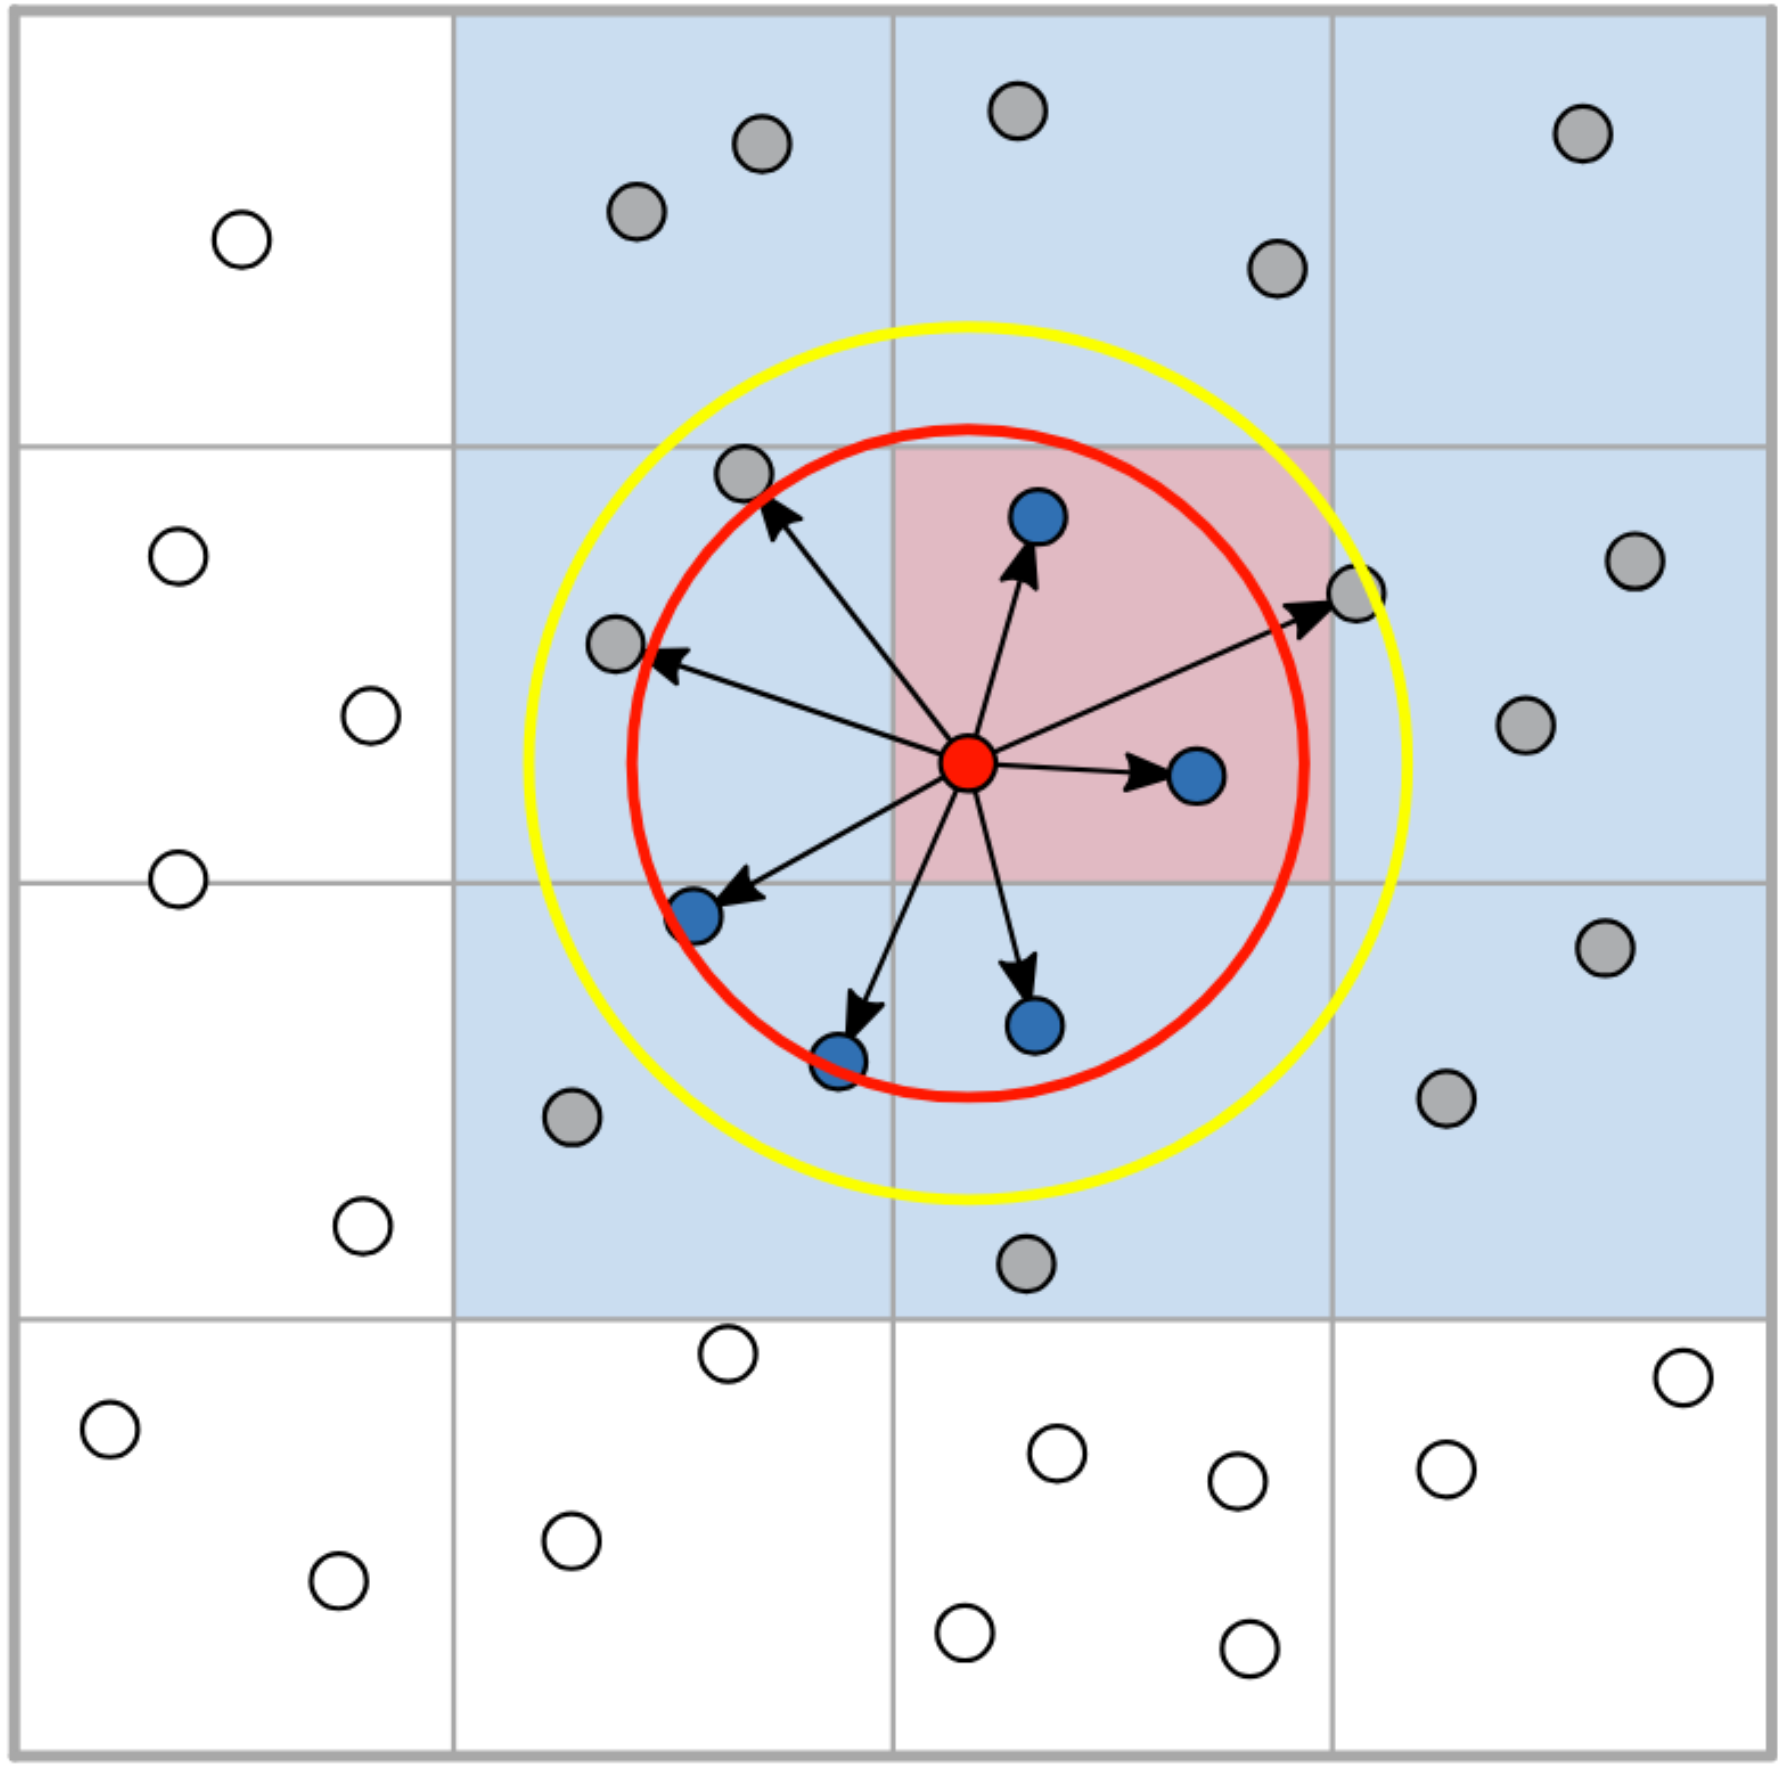
\includegraphics[width=\linewidth]{imgs/verletlists.png}
        \caption{\scriptsize Verlet Lists}
        \label{fig:verletlists}
    \end{subfigure}
    \hfill
    % Fourth Figure
    \begin{subfigure}{0.22\textwidth}
        \centering
        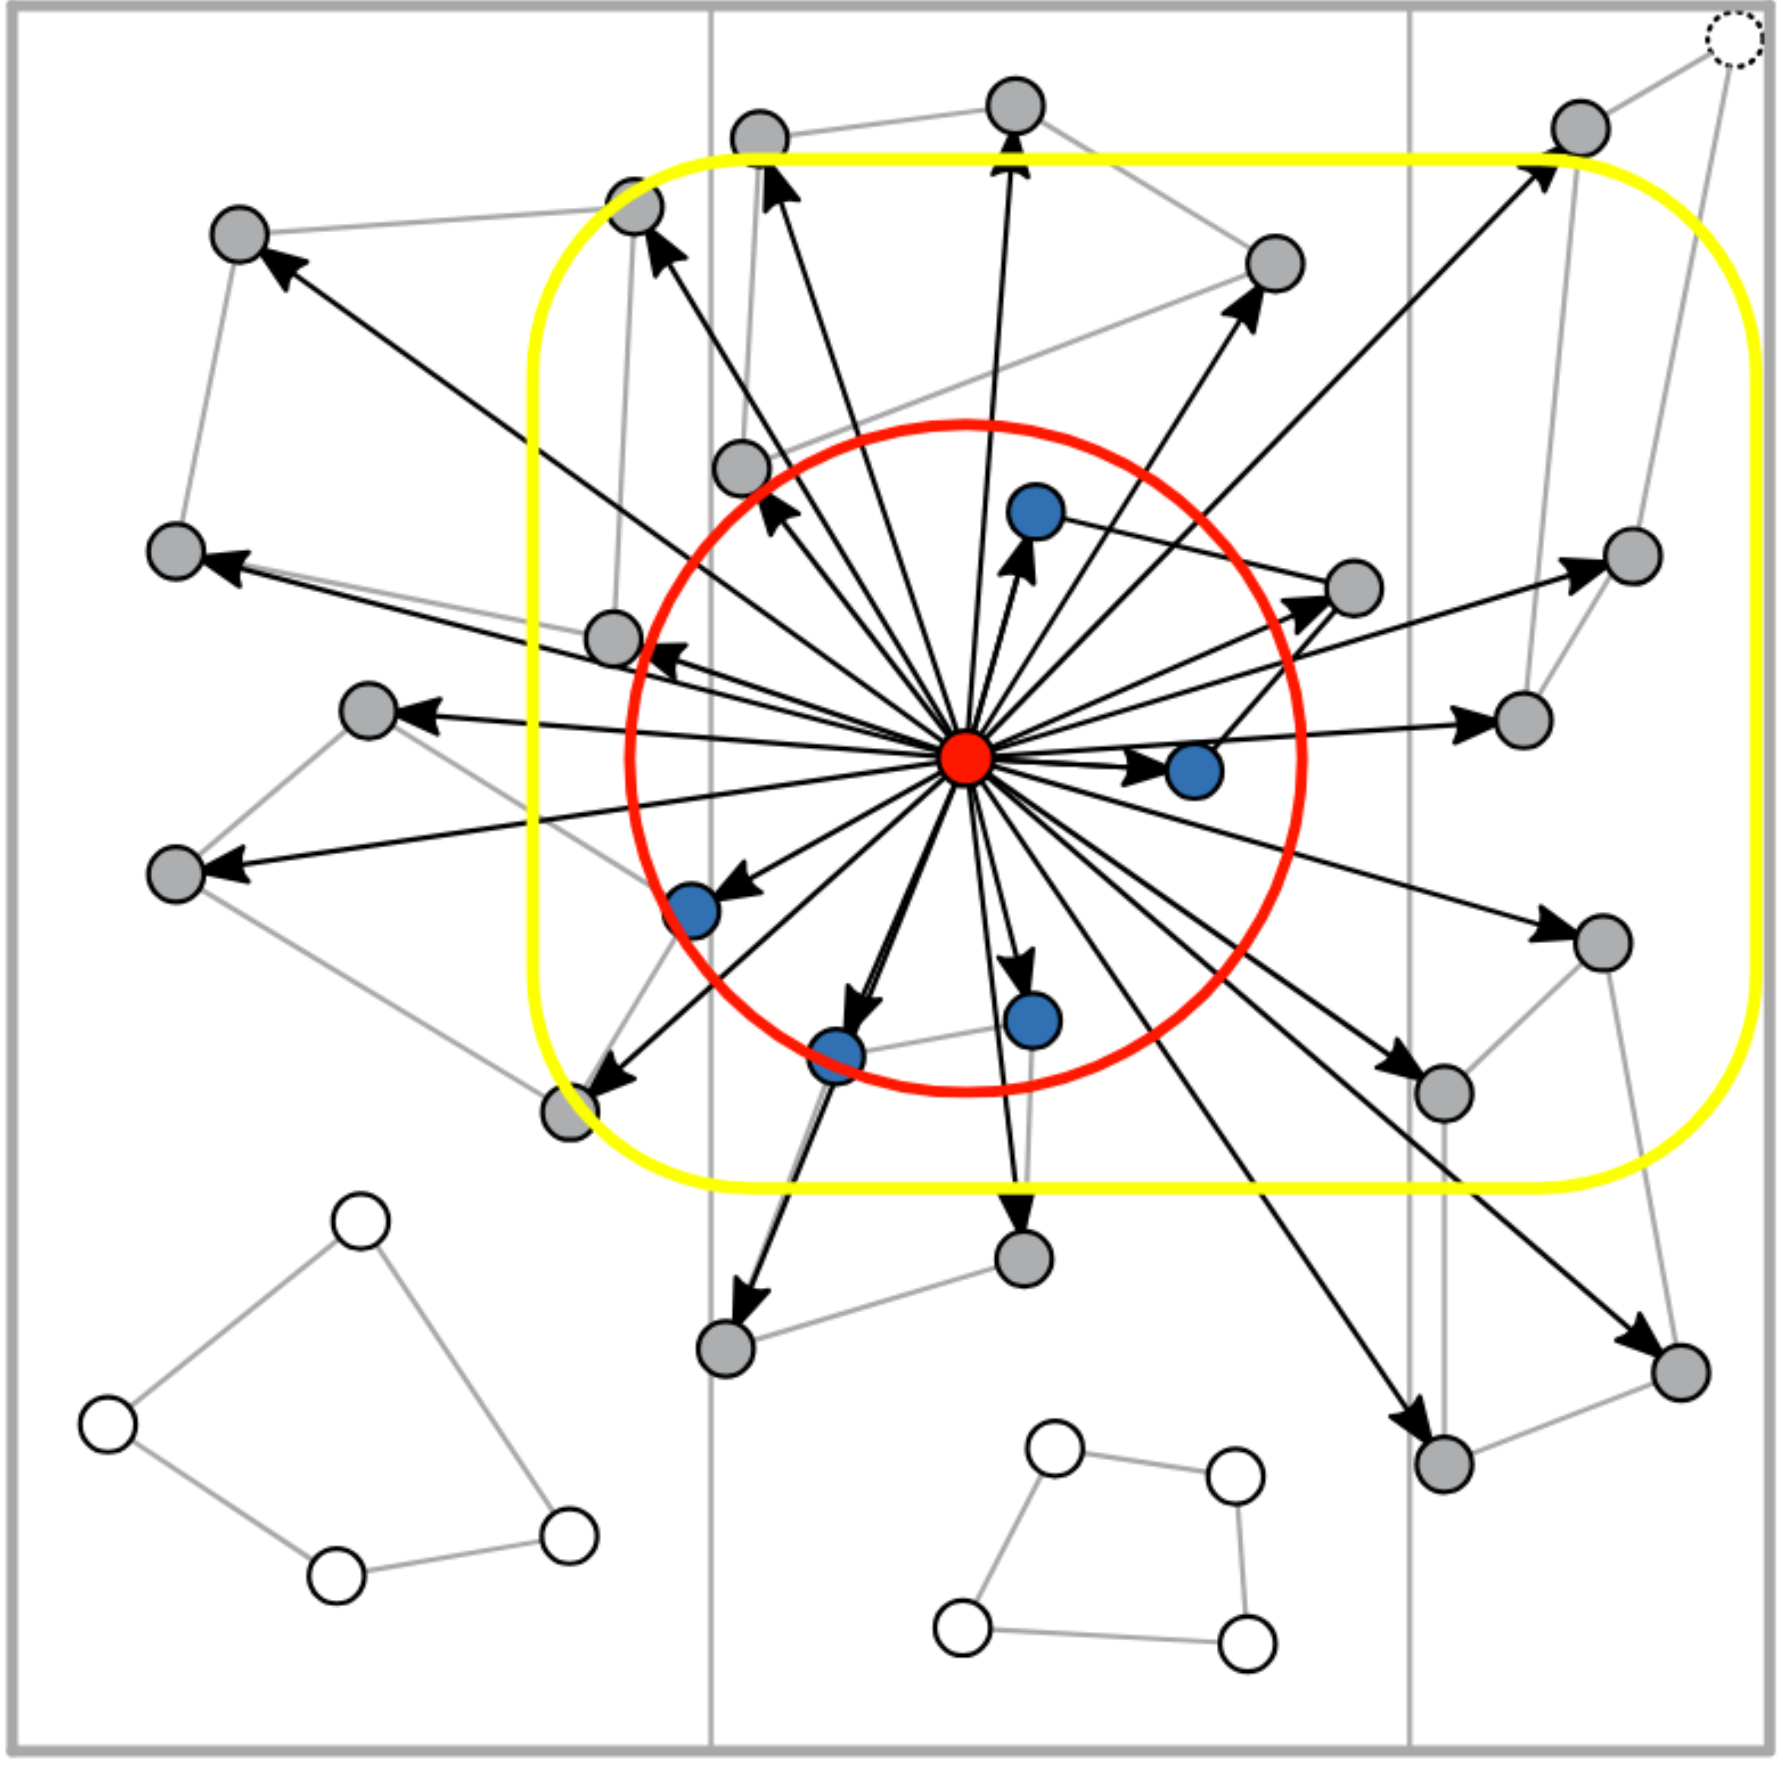
\includegraphics[width=\linewidth]{imgs/verletclusters.png}
        \caption{\scriptsize Verlet Cluster Lists}
        \label{fig:verletclusters}
    \end{subfigure}
    \caption{Neighbor Identification Algorithms in AutoPas \parencite{gratl2022n}}
\end{figure}



\subsection{Traversals}

Traversals determine the order in which particle interactions are computed. AutoPas supports a variety of traversal strategies, each specific to the container being used. These strategies are designed to optimize performance by parallelizing the traversal process, while avoiding race conditions and minimizing the need for schedulers or locking mechanisms \parencite{gratl2019autopas}.

Traversal strategies in AutoPas utilize different cell strategies as their base step. The goal of these base steps is to divide and color the cells of the domain, such that particles in cells of the same color can be processed independently by separate threads. Currently, AutoPas implements three types of base steps: c01, c18, and c08; however, for this thesis, only c01 and c08 are relevant.

\subsection{Base Steps in AutoPas}

\subsubsection{c01 Base Step} The c01 base step uses only a single color, as illustrated in Figure \ref{fig:c01}, and calculates interactions for all neighboring cells without utilizing the Newton3 optimization. In this approach, each cell is assigned to a thread, which calculates the interactions with particles in the neighboring cells. This strategy is highly parallelizable.

% \subsubsection{c18 Base Step} The c18 base step assigns one of 18 colors to each cell, ensuring that no two neighboring cells share the same color. By utilizing the Newton3 optimization, the number of interactions to be calculated is reduced by half. Instead of processing all neighbors, it focuses only on neighbors with a higher index (see Figure~\ref{fig:c18}). This reduces the overall number of computations, however increases the area where race conditions need to be managed, limiting parallel execution.

\subsubsection{c08 Base Step} As the name suggests, the c08 base step uses 8 colors. It is similar to c18 but reduces the locked area further by limiting diagonal interactions and focusing on only four cells (see Figure~\ref{fig:c08}). This adjustment allows for better parallel processing and improved cache utilization.


\subsection{Traversal Strategies}
This thesis focuses on the traversals \texttt{lc\_c08}, \texttt{vlc\_c08}, and \texttt{vcl\_c06}, as they were extensively used in the experiments conducted. A detailed explanation of these strategies is provided below. For information on all traversal strategies, refer to \parencite{gratl2022n}.

\subsubsection{\texttt{lc\_c08}}
This traversal utilizes \texttt{c08} as its base step, and it is designed for the Linked Cells container. It divides a 2D domain into four colors and a 3D domain into eight colors. The dependency of the number of colors \(C\) on the number of dimensions \(D\) follows \(C = 2^D\) \parencite{gratl2022n}.

\subsubsection{\texttt{vlc\_c08}}
This traversal applies the \texttt{c08} base step to each individual cell. To ensure thread safety, a domain coloring consisting of eight colors is used. For each cell, all neighbor lists are processed. Depending on whether the lists were built with Newton3, the base step used is either c01 or c08. \parencite{AutoPasDocs}

\subsubsection{\texttt{vcl\_c06}}
This traversal is used for Verlet Cluster Lists, and it employs a 2D coloring scheme with a stride of \(x = 3\) and \(y = 2\), resulting in six colors (\(3 \times 2 = 6\)). Interactions within clusters are always computed using Newton3, regardless of whether Newton3 is enabled or disabled for the overall traversal. \parencite{AutoPasDocs}

\begin{figure}[htbp]
    \centering
    \begin{subfigure}[b]{0.25\textwidth}
        \centering
        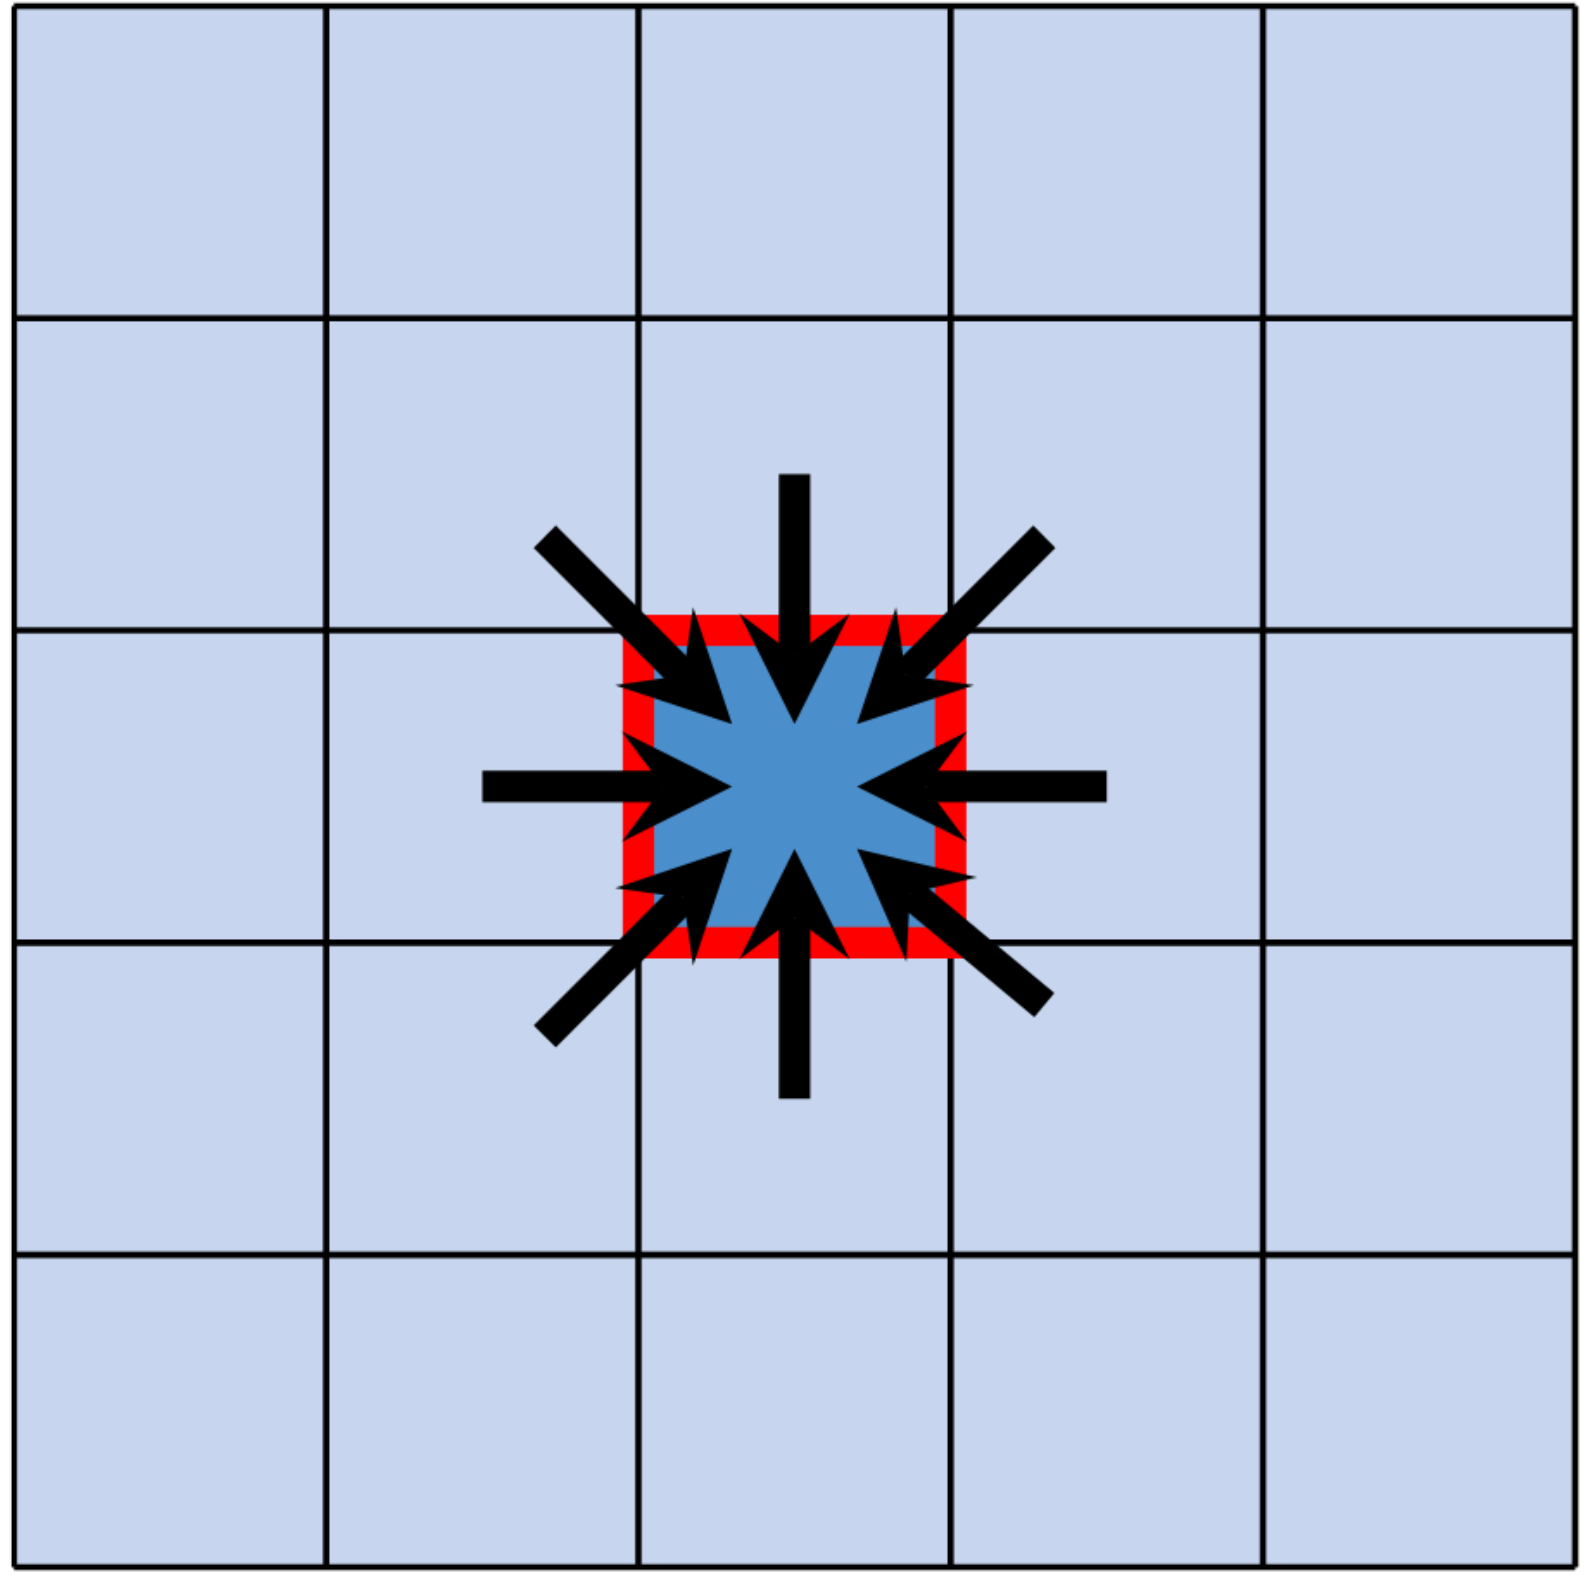
\includegraphics[width=\linewidth]{imgs/c01.png}
        \caption{\scriptsize c01 base step}
        \label{fig:c01}
    \end{subfigure}
    % \begin{subfigure}[b]{0.3\textwidth}
    %     \centering
    %     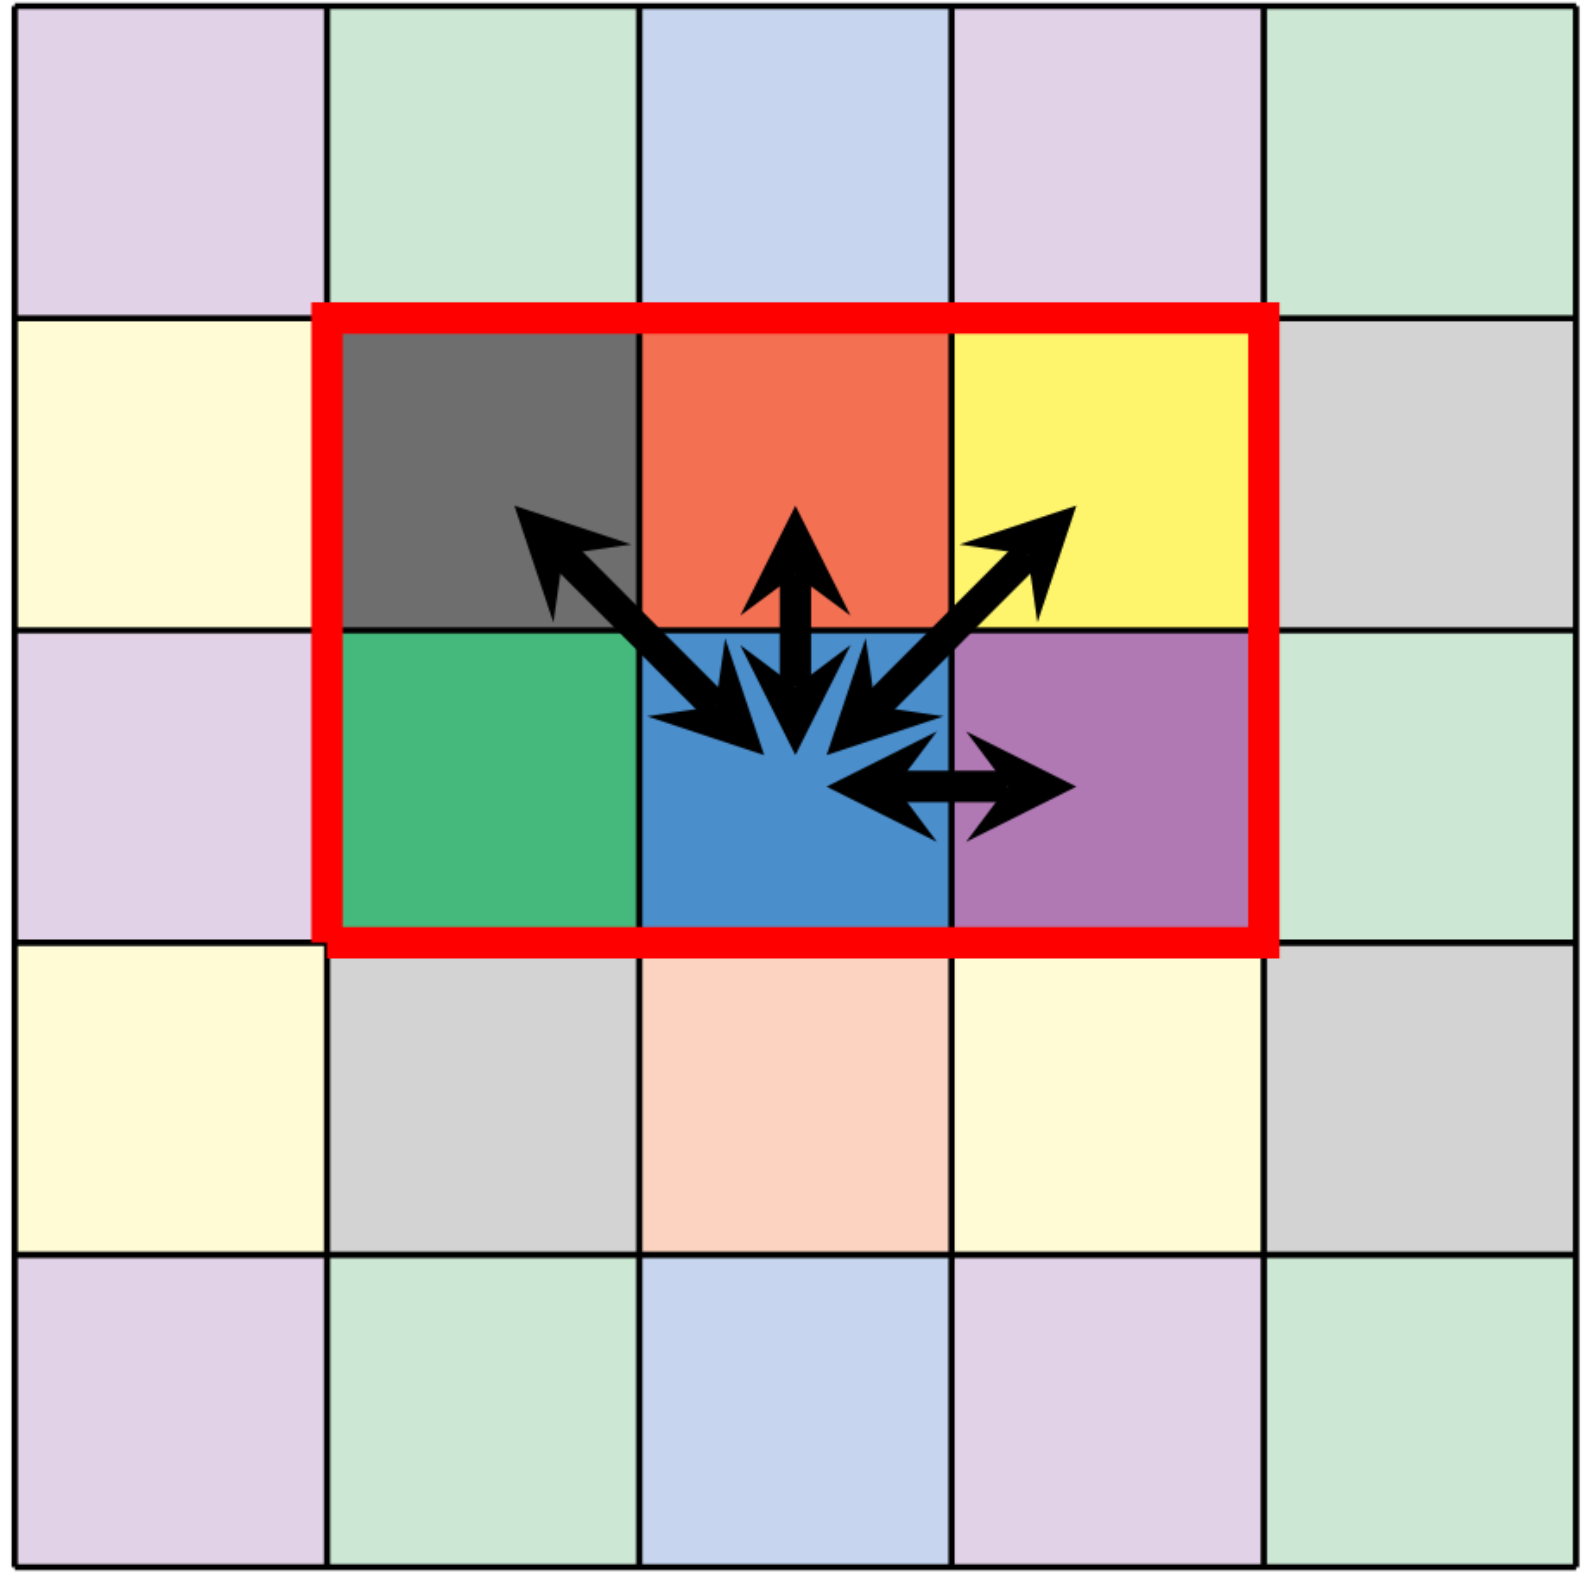
\includegraphics[width=\linewidth]{imgs/c18.png}
    %     \caption{\scriptsize c18 base step}
    %     \label{fig:c18}
    % \end{subfigure}
    \hspace{1em}
    \begin{subfigure}[b]{0.25\textwidth}
        \centering
        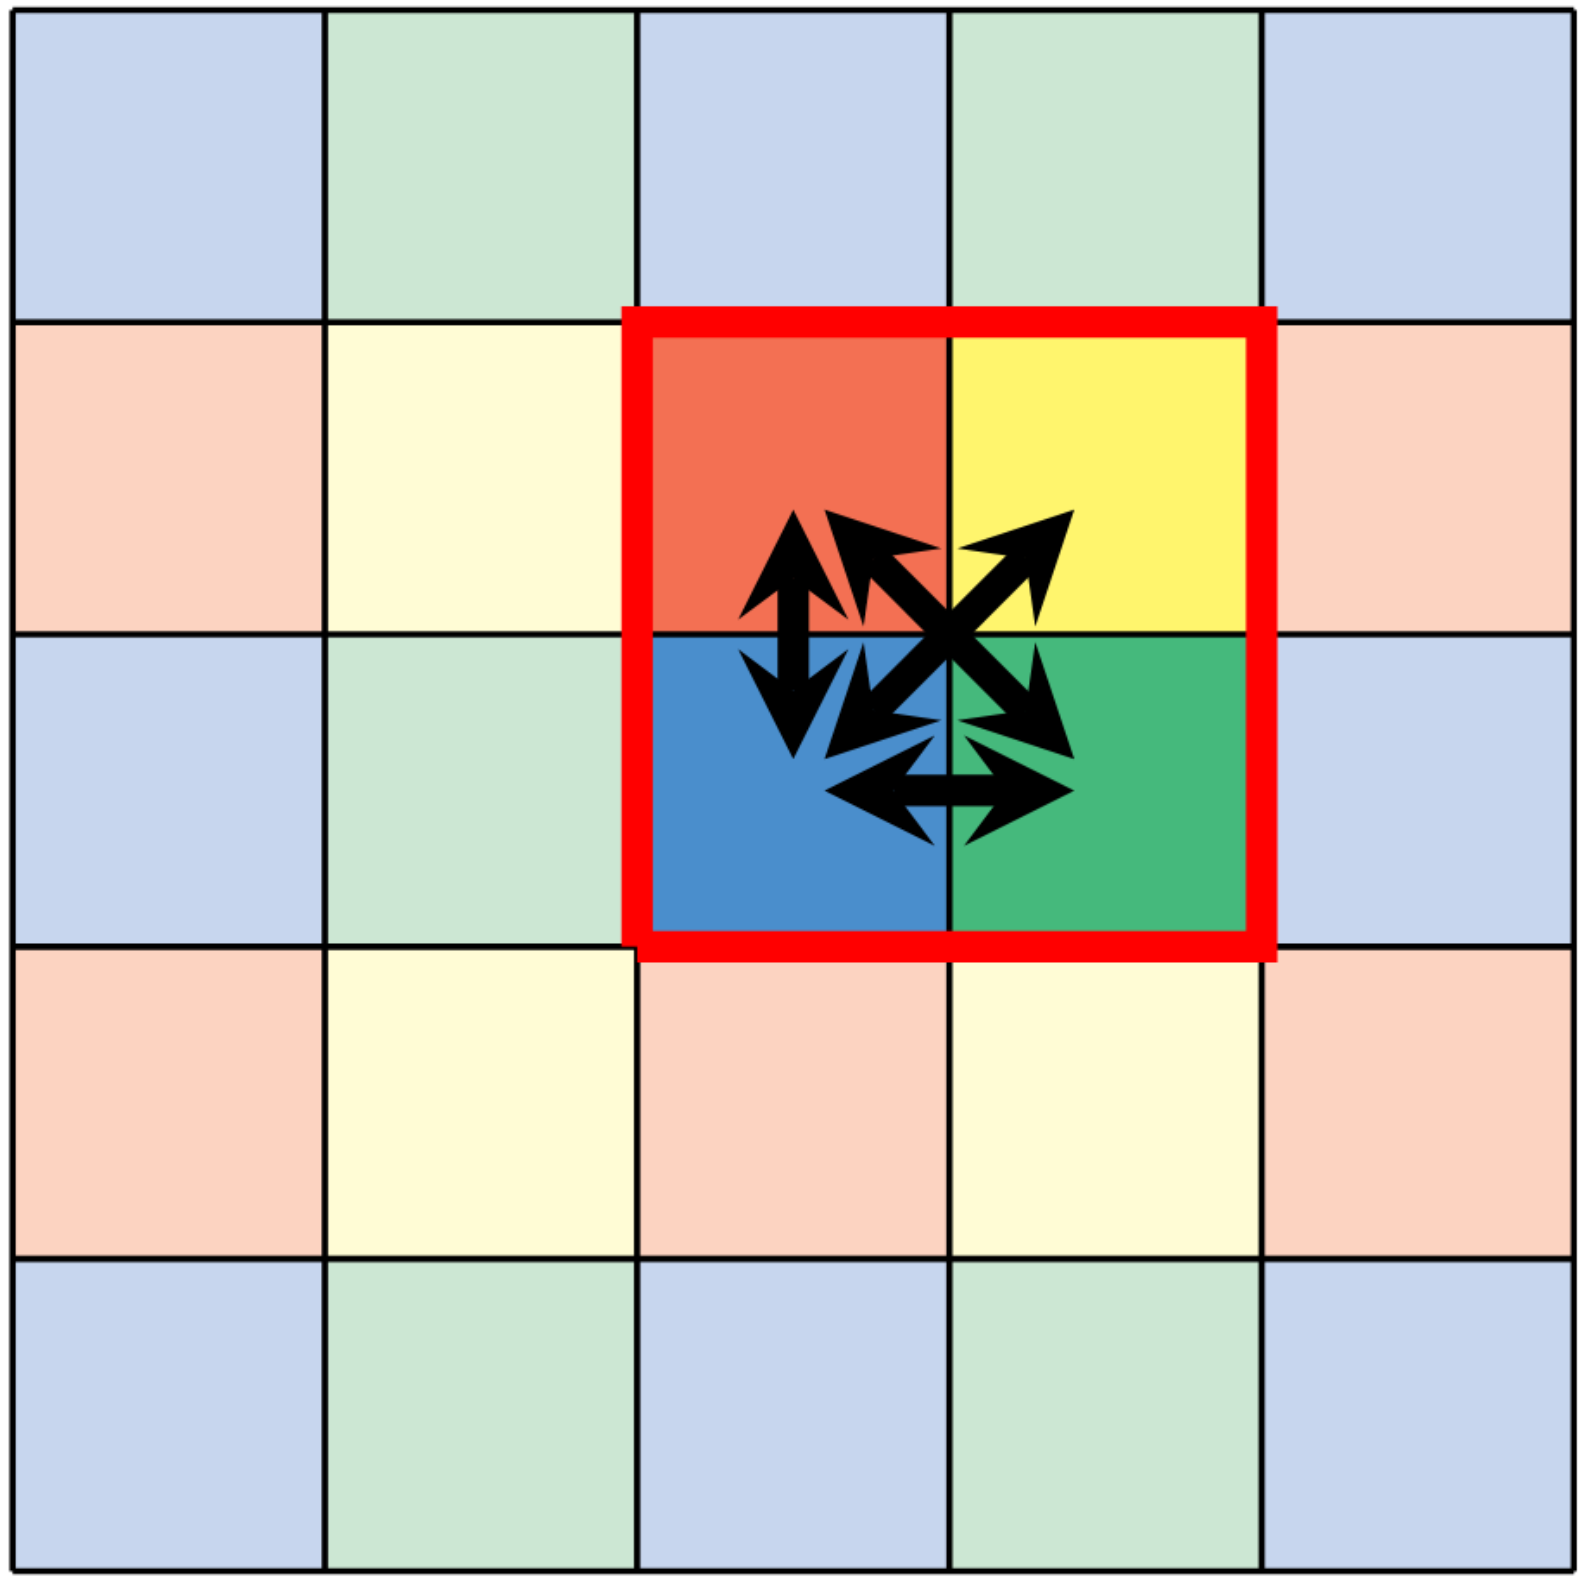
\includegraphics[width=\linewidth]{imgs/c08.png}
        \caption{\scriptsize c08 base step}
        \label{fig:c08}
    \end{subfigure}
    \caption{Base Step Approaches \parencite{newcome2023towards}}
\end{figure}



\subsection{Auto-Tuning}

One of the key features of AutoPas is its auto-tuning capability. Choosing the optimal combination of container and traversal for a simulation can be challenging, especially since different parts of the simulation may benefit from different configurations. AutoPas automates this process, relieving the user of the need to determine the best setup manually.

At the beginning of a simulation, AutoPas tests various configurations over a few iterations, measuring their performance. To reduce overhead, configurations using the same container are tested consecutively. This approach assumes that the state of the simulation remains relatively stable over consecutive time steps, making the performance results comparable. Importantly, the results of these initial tests are not discarded but are used in the following iterations \parencite{gratl2019autopas}.

After evaluating multiple configurations, AutoPas selects the best-performing setup and uses it for a user-defined number of iterations. Following this period, the system enters a re-tuning phase, where a new configuration may be selected based on how the simulation has evolved.








\subsection{Particle Types}

In AutoPas, there are three types of particles: Owned, Halo, and Dummy particles.  
\begin{itemize}
    \item Owned particles are the primary particles managed by the current AutoPas instance. These represent the actual simulation particles within a subdomain.  
    \item Halo particles are not owned by the current AutoPas object but exist at the borders of subdomains. Since they interact with particles in neighboring domains, they must be duplicated and made available in neighboring subdomains to ensure the correct computation of forces. During force calculations, halo particles serve as interaction partners like any other particle, but their forces are only computed in the domain that owns them.  
    \item Dummy particles represent deleted particles. They do not participate in force calculations.

\end{itemize}


\subsection{Interaction Computation in AutoPas} \label{sec:interaction_comp}

Two important buffers are used in AutoPas: the particle buffer and the halo particle buffer. The particle buffer stores particles that should not yet be added to the container. The halo particle buffer holds halo particles, making sure that particles at the boundaries of subdomains are available for correct force calculations.


In AutoPas, interactions are computed in two stages so that all particles are correctly accounted for during the simulation.

\begin{enumerate}
    \item \textbf{Container Interactions}: The main function \texttt{computeInteractions(\&traversal)} calculates interactions for particles within the container. This involves iterating over particle pairs, triplets, or higher multiples, ensuring efficient resolution of regular particle interactions.

    \item \textbf{Buffer Interactions}: Interactions for particles in the buffers are computed separately using the \texttt{computeRemainderInteractions(functor, newton3)} function. This step ensures that particles in the buffer interact correctly with container particles and among themselves. The following types of interactions are handled:
    \begin{itemize}
        \item \textbf{Particle Buffer \(\leftrightarrow\) Container}: Interactions between buffer particles and container particles.
        \item \textbf{Halo Particle Buffer \(\rightarrow\) Container}: Interactions from halo particle buffers to container particles.
        \item \textbf{Particle Buffer \(\leftrightarrow\) Particle Buffer}: Interactions among buffer particles.
        \item \textbf{Halo Particle Buffer \(\rightarrow\) Particle Buffer}: Interactions from halo particle buffers to buffer particles.
    \end{itemize}
\end{enumerate}

% This two-stage computation guarantees accurate interaction handling for all particles, including those in the buffers. Explicit handling of buffer particles allows the simulation to avoid unnecessary neighbor list rebuilds, maintaining computational efficiency.




\chapter{Related Work}
As discussed in the previous chapters, a significant portion of the computational time in molecular dynamics simulations is spent on calculating pairwise force interactions between particles. A common optimization technique is to store the nearby particles, which in the case of Verlet Lists involves maintaining neighbor lists, as previously explained.

Since rebuilding these neighbor lists is computationally expensive, several works have focused on reducing this overhead. One such approach was presented in a previous thesis by Luis Gall \parencite{gall2023exploration}.

Gall's work primarily focused on reducing the time spent on neighbor list rebuilds. To achieve this, he proposed a dynamic rebuild criterion that adapts based on particle movement, triggering updates only when necessary. This approach was advantageous for scenarios with a high velocity difference over time.

Furthermore, Gall focused on a partial rebuild strategy, where only the neighbor lists affected by particle movement were updated. This method proved to be advantageous in large simulation domains, for a small Verlet skin size. 


Beyond AutoPas, several molecular dynamics simulators also implement the neighbor indetification algorithms described in Section \ref{sec:neighbor_iden_algs}. Examples include:

\begin{itemize}
    \item LS1 MarDyn - A Linked Cells-based simulator optimized for large-scale parallel molecular dynamics simulations. \parencite{niethammer2014ls1}
    \item LAMMPS - A molecular dynamics software package that employs Verlet Lists. \parencite{thompson2022lammps}
    \item GROMACS - A high-performance molecular dynamics package that utilizes Verlet Cluster Lists. \parencite{abraham2015gromacs}
\end{itemize}

Unlike AutoPas, which dynamically selects the best suited algorithm based on runtime performance using tuning, these pieces of software rely on fixed algorithms that are optimized for specific types of simulations. While this allows them to be highly efficient in their intended use cases, they lack the flexibility to adapt to varying simulation conditions.



\chapter{Implementation}
\section{Initial Problem}
Simulations in AutoPas are configured using parameters specified in a \texttt{.yaml} file, which defines the conditions of the simulation. Examples of such files can be found in the appendix \ref{sec:appendix}. The key fields relevant to this thesis are:

\begin{verbatim}
container                        : # List of containers to choose from
verlet-rebuild-frequency         : # Frequency of neighbor list rebuilds
verlet-skin-radius               : # Distance within which a particle is 
                                   # stored in the neighbor list
data-layout                      : # Data storage format (AoS or SoA)
traversal                        : # List of traversals to choose from
newton3                          : # Boolean value determining if Newton's 
                                   # third law is enabled
iterations                       : # Number of iterations
\end{verbatim}

Rebuilding neighbor lists is computationally expensive, so it is advantageous to reuse these lists for as many iterations as possible. Neighbor lists are generated for each particle, containing references to all particles within the cutoff range. To enable extended use, particles slightly beyond the cutoff radius are included in the neighbor list by extending the radius with a region called the "Verlet skin," which is also configurable in the 	\texttt{.yaml} file.

If particles move faster than half the defined Verlet skin distance, they may enter the cutoff region of other particles, invalidating the neighbor lists. Even if a single particle among hundreds of thousands exceeds this threshold, all neighbor lists must be rebuilt, incurring high computational costs. 

This thesis investigates whether storing fast-moving particles in a buffer temporarily, instead of rebuilding the neighbor lists immediately, can reduce computational overhead. The objective is to evaluate the potential of this approach for future optimization and research.

\section{Particle Buffer}

\subsection{Particle Buffer Mechanism}

In AutoPas, each iteration involves a call to the 	\texttt{updateContainer()} function, which performs several tasks, including:
\begin{itemize}
    % \item Deleting halo particles.
    \item Removing particles that no longer belong in the container.
    \item Checking whether the neighbor lists are invalid, based on criteria such as the 	\texttt{verlet-rebuild-frequency}, tuning iterations, or the presence of fast particles.
\end{itemize}


The particle buffer is implemented as a 	\texttt{std::vector<FullParticleCell<Particle>>}, where each thread has its own buffer, enabling efficient multithreading. This buffer temporarily stores particles that should not yet be added back to the container. A corresponding halo particle buffer stores particles not owned by the current AutoPas object.

The function \texttt{checkNeighborListsInvalidDoDynamicRebuild()} is responsible for 
checking fast particles and is called within \texttt{updateContainer()}. It operates by iterating through owned particles in the container. For each particle, the displacement squared relative to the Verlet skin squared is calculated. If the displacement exceeds the threshold, the particle is marked for buffering. A copy of the particle is added to the buffer, and the original is marked as deleted to maintain neighbor list integrity. Marked particles, referred to as "dummy particles," are ignored in computations and eventually removed from the container.

This mechanism mitigates the cost of frequent neighbor list rebuilds by deferring the integration of fast particles until the next scheduled rebuild. During a rebuild, the buffer is cleared, and its particles are integrated into the neighbor lists.

\begin{lstlisting}[style=cppstyle]
template <typename Particle>
void LogicHandler<Particle>::checkNeighborListsInvalidDoDynamicRebuild() {

 AUTOPAS_OPENMP(parallel reduction(or : _neighborListInvalidDoDynamicRebuild))
  for (auto iter = this->begin(IteratorBehavior::owned | IteratorBehavior::containerOnly); iter.isValid(); ++iter) {
    const auto distance = iter->calculateDisplacementSinceRebuild();
    const double distanceSquare = utils::ArrayMath::dot(distance, distance);

      if (distanceSquare >= halfSkinSquare) {

      Particle& particle = *iter;
      Particle particleCopy = particle;

       _particleBuffer[autopas_get_thread_num()].addParticle(particleCopy);
        internal::markParticleAsDeleted(particle);

        _particleNumber++;
      }
  }
  ....
}
\end{lstlisting}

\subsection{Interaction Computation}
During the simulation, interactions are computed in two distinct stages:

\begin{enumerate}
    \item \textbf{Container Interactions}: The main function \texttt{computeInteractions(\&traversal)} calculates interactions for particles within the container. This involves iterating over particle pairs, triplets, or higher multiples, ensuring efficient resolution of regular particle interactions.

    \item \textbf{Buffer Interactions}: Interactions for particles in the buffers are computed separately using the \texttt{computeRemainderInteractions(functor, newton3)} function. This step ensures that particles in the buffer interact correctly with container particles and among themselves. The following types of interactions are handled:
    \begin{itemize}
        \item \textbf{Particle Buffer \(\leftrightarrow\) Container}: Interactions between buffer particles and container particles.
        \item \textbf{Halo Particle Buffer \(\rightarrow\) Container}: Interactions from halo particle buffers to container particles.
        \item \textbf{Particle Buffer \(\leftrightarrow\) Particle Buffer}: Interactions among buffer particles.
        \item \textbf{Halo Particle Buffer \(\rightarrow\) Particle Buffer}: Interactions from halo particle buffers to buffer particles.
    \end{itemize}
\end{enumerate}

This two-stage computation ensures accurate interaction handling for all particles, including those in the buffers. Explicit handling of buffer particles allows the simulation to avoid unnecessary neighbor list rebuilds, maintaining computational efficiency.

\section{DeleteFunction}
Initially, in \texttt{checkNeighborListsInvalidDoDynamicRebuild()}, particles were marked as deleted in the container, and a copy was created and added to the buffer. While this approach works for containers like Verlet Lists, as it preserves the integrity of the neighbor lists, it introduces overhead for containers such as LinkedCells. In the case of LinkedCells, every fast-moving particle results in the creation of a dummy particle within the container, depending on the simulation, potentially leading to a significant accumulation of these dummies until they are disregarded. 

This issue could become problematic when simulations involve combined usage of LinkedCells and VerletLists. To address this, the hypothesis was to minimize the overhead caused by dummy particles when using containers like LinkedCells.

The available delete functions at the time were:
\begin{lstlisting}[style=cppstyle]
bool deleteParticle(size_t cellIndex, size_t particleIndex);
bool deleteParticle(Particle &particle);
\end{lstlisting}

These functions could not be directly used within the parallel loop. For certain containers, the delete operation employs a swap-delete mechanism, where the particle to be deleted is swapped with the last particle in the cell before being removed. This implementation, while efficient, is not thread-safe within a parallel loop.

One proposed solution was to gather all particles marked for deletion into a separate buffer and process them sequentially after the parallel loop. However, this approach proved infeasible for the first function, as the indices of remaining particles change dynamically when deletions occur, making it too time-consuming to update and track these indices. For the second function, attempts to store references or pointers to the particles encountered issues when multiple particles were deleted from the same vector. This led to invalid references, as deletions could shift the positions of particles in memory.

To resolve these issues, a new delete function was implemented:
\begin{lstlisting}[style=cppstyle]
deleteParticle(int id, size_t cellIndex);
\end{lstlisting}

\subsection{Updated Code}
The updated implementation ensures safe handling of deletions within a parallel loop by temporarily storing particle IDs and their cell indices in a buffer. After the loop, a sequential process iterates through this buffer to perform deletions:

\begin{lstlisting}[style=cppstyle]
template <typename Particle>
void LogicHandler<Particle>::checkNeighborListsInvalidDoDynamicRebuild() {

AUTOPAS_OPENMP(parallel reduction(or : _neighborListInvalidDoDynamicRebuild))
  for (auto iter = this->begin(IteratorBehavior::owned | IteratorBehavior::containerOnly); iter.isValid(); ++iter) {
    ...

      if (distanceSquare >= halfSkinSquare) {

        Particle& particle = *iter;
        Particle particleCopy = particle;

       _particleBuffer[autopas_get_thread_num()].addParticle(particleCopy);

        size_t cellIndex = iter.getVectorIndex();
        toDelete[autopas_get_thread_num()].push_back(std::make_tuple(particle.getID(), cellIndex));

        _particleNumber ++;
      }
  }

  for (const auto& t : toDelete) {
    for (auto p : t) {
      int id = std::get<0>(p);
      size_t cellIndex = std::get<1>(p);
      _containerSelector.getCurrentContainer().deleteParticle(id, cellIndex);
    }
  }

  ....
}
\end{lstlisting}

\subsection{Implementation Details}
The new delete function was implemented in several container classes, including \texttt{DirectSum.h}, \texttt{LinkedCells.h}, \texttt{LinkedCellsReferences.h}, \texttt{VerletClusterLists.h}, \\ \texttt{VerletListsLinkedBase.h}, and \texttt{Octree.h}. Below are examples from two of these classes:

\subsubsection{In 	\texttt{LinkedCells.h}}
The swap-delete method is used here to efficiently manage particle deletions:
\begin{lstlisting}[style=cppstyle]
bool deleteParticle(int id, size_t cellIndex) override {
  auto &particleVec = this->_cells[cellIndex]._particles;

  for (auto &particle : particleVec) {
    if (particle.getID() == id) {
      const bool isRearParticle = &particle == &particleVec.back();

      particle = particleVec.back();
      particleVec.pop_back();

      return !isRearParticle;
    }
  }
}
\end{lstlisting}

\subsubsection{In 	\texttt{VerletListsLinkedBase.h}}
Here, particles are marked as deleted to avoid interfering with the internal structures of the Verlet Lists:
\begin{lstlisting}[style=cppstyle]
bool deleteParticle(int id, size_t cellIndex) override {
  auto &particleVec = _linkedCells.getCells()[cellIndex]._particles;
  for (auto &particle : particleVec) {
    if (particle.getID() == id) {
      internal::markParticleAsDeleted(particle);
      return false;
    }
  }
}
\end{lstlisting}

The remaining implementations for other containers follow a similar structure. The full code can be found on \href{https://github.com/AutoPas/AutoPas/commit/d251b0ab8544a76f4e8150bf5e91c09d874d4f4c}{\texttt{GitHub}}. 


\section{CSV File}

By enabling the CMake flag \texttt{LOG\_ITERATIONS}, the simulation generates a \texttt{.csv} file containing valuable information for each iteration. This data provides insights into the performance and configuration of the simulation. The header fields included in the file are as follows:

\begin{multicols}{2}
\raggedright
\texttt{
Date \\
Iteration \\
Functor \\
inTuningPhase \\
Interaction Type \\
Container \\
CellSizeFactor \\
Traversal \\
Load Estimator \\
Data Layout \\
Newton 3 \\
computeInteractions[ns] \\
remainderTraversal[ns] \\
rebuildNeighborLists[ns] \\
computeInteractionsTotal[ns] \\
tuning[ns]
}
\end{multicols}




Among these, the fields \textit{computeInteractions[ns]}, \textit{remainderTraversal[ns]}, and \textit{rebuildNeighborLists[ns]} are of particular importance for tracking the computational time spent on interaction calculations in the container and in the fast particle buffer.

To facilitate further analysis of performance, three additional fields were introduced:
\begin{itemize}
    \item \textbf{numberOfParticlesInContainer}: Records the total number of particles currently in the container.
    \item \textbf{numberFastParticles}: Tracks the number of fast-moving particles identified in each iteration.
    \item \textbf{particleBufferSize}: Indicates the size of the particle buffer.
\end{itemize}

These new fields allow us to quantify the behavior of fast particles, evaluate the efficiency of the buffer, and compare the number of fast particles with the total particles in the container. 

\chapter{Performance}
% withtuning experiments
%     - freq exp
%     - iter exp
%     - analyze
% notuning exp
%     - vlc c08
%     - lc c08
%     - vcl c06
%     - why chosen? adv? how they work in tehcnical background
% percentage expr
%     - why only run in some of them
%     - why still not performat
%     - why chose to use spinodal all of a sudden 
%     - idea to converge to DVL
%     - is the slight improvement only a coincidence - repeating the tests many times
%     - idea to increase the temperatur in spinodial decomp 
% Profiler
% add where to find the tests on github and such, also attach slurm job maybe
%add in which cluster each experiment was ran on


This chapter explores whether the use of the fast particle buffer provides measurable advantages by presenting the results of various experiments conducted under different scenarios. It details the experimental setup, including the working environment, explains the rationale behind the selection of specific experiments, and provides an analysis of the observed outcomes. Due to the high number of experiments conducted, only the most relevant graphs and data are presented here. However, the complete dataset, along with all scripts used for plotting and analysis, is available in the accompanying \href{https://github.com/xhulia028/GraphView}{\texttt{GitHub repository}}.

% ======================================================================
\section{Test System Specifications}

The initial experiments were conducted on the CoolMUC2 Linux cluster at the Leibniz Supercomputing Centre (LRZ), TUM. This cluster operated on the SLES15 SP1 Linux OS and consisted of 812 nodes, each equipped with 28 cores running at a nominal frequency of 2.6 GHz with two hyperthreads per core \parencite{coolmuc2}. The \texttt{cm2\_tiny} partition was used for these experiments. Unfortunately, due to a severe hardware failure, CoolMUC2 was decommissioned during the course of this work.

Subsequent experiments were performed on CoolMUC4, the successor to CoolMUC2. CoolMUC4 features Intel® Xeon® Platinum 8380 CPUs (Ice Lake) with 112 cores per node, 512 GB of RAM, and a nominal core frequency of 3.0 GHz (ranging from 0.8 to 4.2 GHz). It operates on the SLES15 SP6 Linux OS \parencite{coolmuc4}. The experiments were run on the \texttt{cm4\_tiny} partition.

The code was compiled with GCC 11.2.0 in CoolMuc2 and GCC 12.2.0 in CoolMuc4. 


% \textbf{MENTION PROFILER and the performance measurements are performed with VTune3 version 2021.7.1 (build
% 619561).}

% ======================================================================
\section{Scenario descriptions}

For the experiments, four different simulations were used, each chosen to assess the impact of the fast particle buffer under various conditions and provide a comprehensive evaluation of its performance.

% \textbf{TESTS CAN BE FOUND IN GITHUB}
% \textbf{Cite Luis' thesis for some of these details; the rest cite AutoPas.}


\subsection{Falling Drop} 
This experiment involves two objects: \texttt{CubeClosestPacked}, which represents a bed of particles, and a sphere of particles. At the start of the simulation, the sphere is accelerated by gravity and falls into the basin. Upon collision, the particles from the sphere mix with those in the basin. This experiment uses reflective boundaries and the Lennard-Jones AVX functor, containing over 15,000 particles. The default YAML configuration for this experiment is set to run for 15,000 iterations; however, as will be discussed later, this parameter is adjusted for specific tests. The initial and final states of the simulation are depicted below \ref{fig:fd}, illustrating the transition from the sphere's descent to the equilibrium state of the mixed particles.

\subsection{Exploding Liquid} The second scenario describes an exploding liquid consisting of a highly compressed and heated liquid film suddenly exposed to a vacuum. This exposure causes the film to rapidly expand and disintegrate into thin filaments and droplets as it destabilizes \parencite{seckler2021autopas}. This experiment consists of approximately 3,800 particles and, by default, runs for 12,000 iterations. Unlike the first scenario, this simulation uses periodic boundaries. A visualization of the system before and after the explosion is provided in Figure~\ref{fig:exl},

\subsection{Constant Velocity Cube} This scenario features a cube that moves at a nearly constant velocity and, by default, runs for 5000 iterations. The cube consists of approximately 50,000 particles, which do not interact with each other as dynamically as in the previous two scenarios. Reflective boundaries are employed in this experiment. Due to the minimal interaction between particles, this scenario was selected to examine the effects of a structured, uniform motion. The goal was to evaluate how the particle buffer performs in such conditions. A visual representation of the cube's motion over time can be found in Figure~\ref{fig:conc}.

\subsection{Spinodal Decomposition Equilibration}
% The fourth scenario examines equilibration. Initially, the system is prepared at a specified temperature and density, ensuring conditions suitable for equilibrium. A velocity-scaling thermostat is applied to regulate the temperature and bring the system to a stable state. During this process, interactions between particles are monitored to ensure proper thermalization and energy distribution. This simulation involves a large number of particles—over 4 million—, and runs for 100'000 iterations. This experiment was chosen due to the high and dynamic interactions between particles, resulting in a significant number of fast particles.

The fourth scenario examines an equilibration simulation, where a GridBlock object populates the domain with particles. The simulation then runs for 100,000 iterations, allowing the particles to reach an equilibrium state. This scenario involves over four million particles and is characterized by high particle interaction dynamics, resulting in a substantial number of fast-moving particles. The evolution of the system to equilibrium is depicted in Figure~\ref{fig:equilibration}.

% \subsection{Spinodal Decomposition Equilibration} The fourth scenario examines spinodal decomposition. Initially, the system is stabilized at a temperature above the critical point and a density near the critical value. A velocity-scaling thermostat is then applied to rapidly cool the system to a temperature well below the critical point. This sudden cooling causes the fluid to become unstable, leading to phase separation into vapor and liquid phases. This scenario involves a large number of particles—over 4 million—and was chosen due to the high and dynamic interactions between particles, resulting in a significant number of fast particles.

% The fourth scenario examines spinodal decomposition equilibration. Initially, the system is stabilized at a temperature above the critical point and a density near the critical value. A velocity-scaling thermostat is then applied to rapidly cool the system to a temperature well below the critical point. This sudden cooling drives the system into an unstable state, leading to spontaneous phase separation into vapor and liquid regions. The simulation is run for a sufficiently long time to allow the system to reach a quasi-equilibrium state, where domain coarsening slows down, and phase-separated structures become more stable. This scenario involves a large number of particles—over 4 million—and was chosen due to the high level of particle interactions, which result in a significant number of fast-moving particles.


\vspace{1em} 
\vspace{1em} 
\vspace{1em} 

\noindent
\begin{minipage}[t]{0.5\textwidth} % Reserve half a row for the first picture
    \centering
    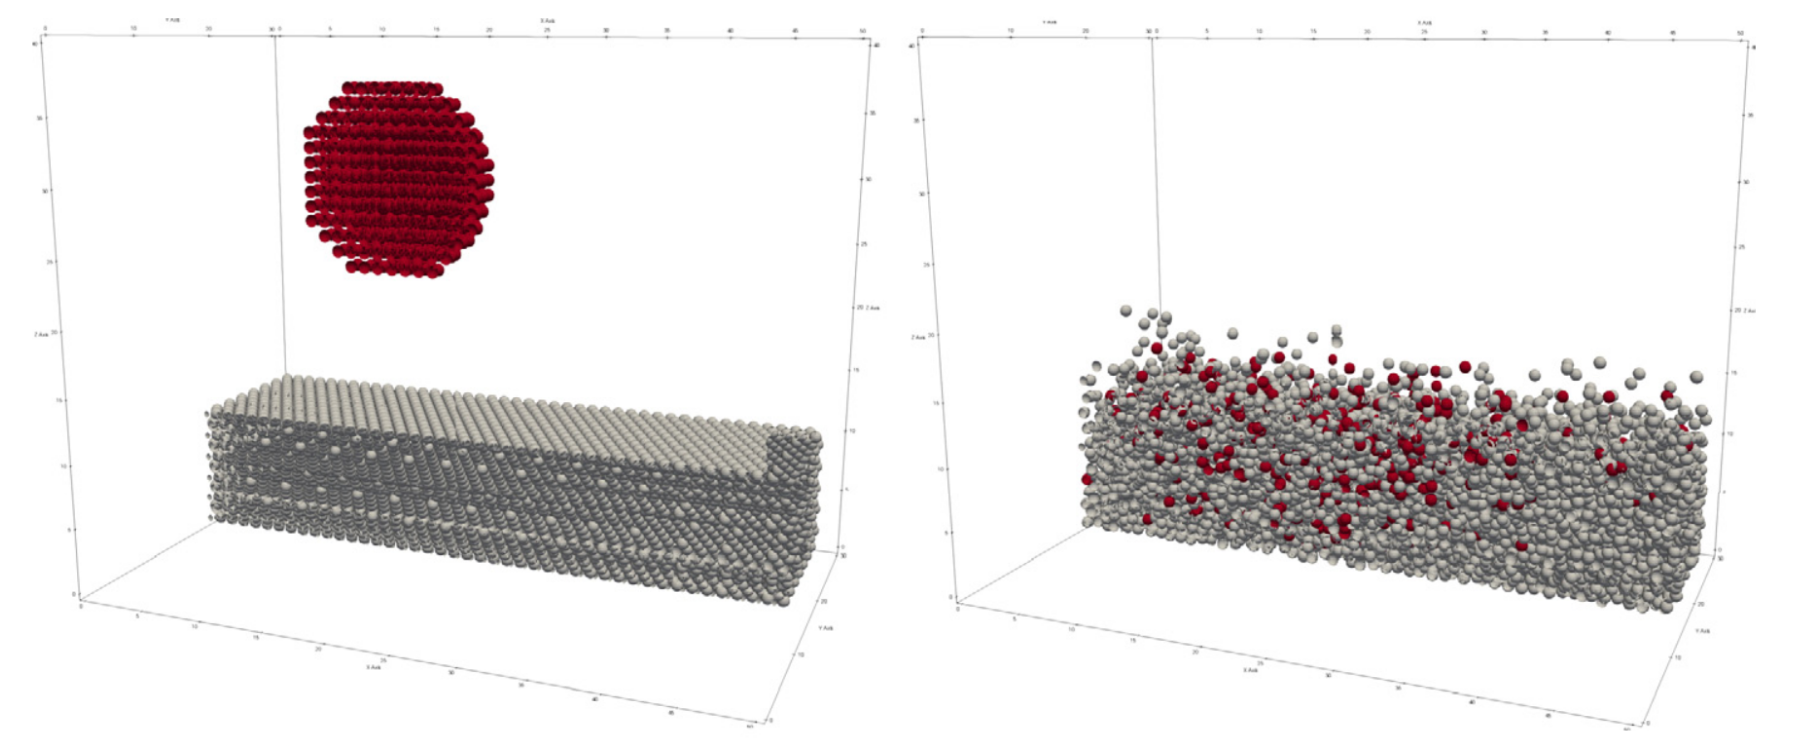
\includegraphics[width=0.9\linewidth]{imgs/fallingDrop.png} % Dynamically scale the image
    \captionof{figure}{Falling Drop \parencite{gratl2022n}}
    \label{fig:fd}
\end{minipage}%
\begin{minipage}[t]{0.5\textwidth} % Reserve half a row for the second picture
    \centering
    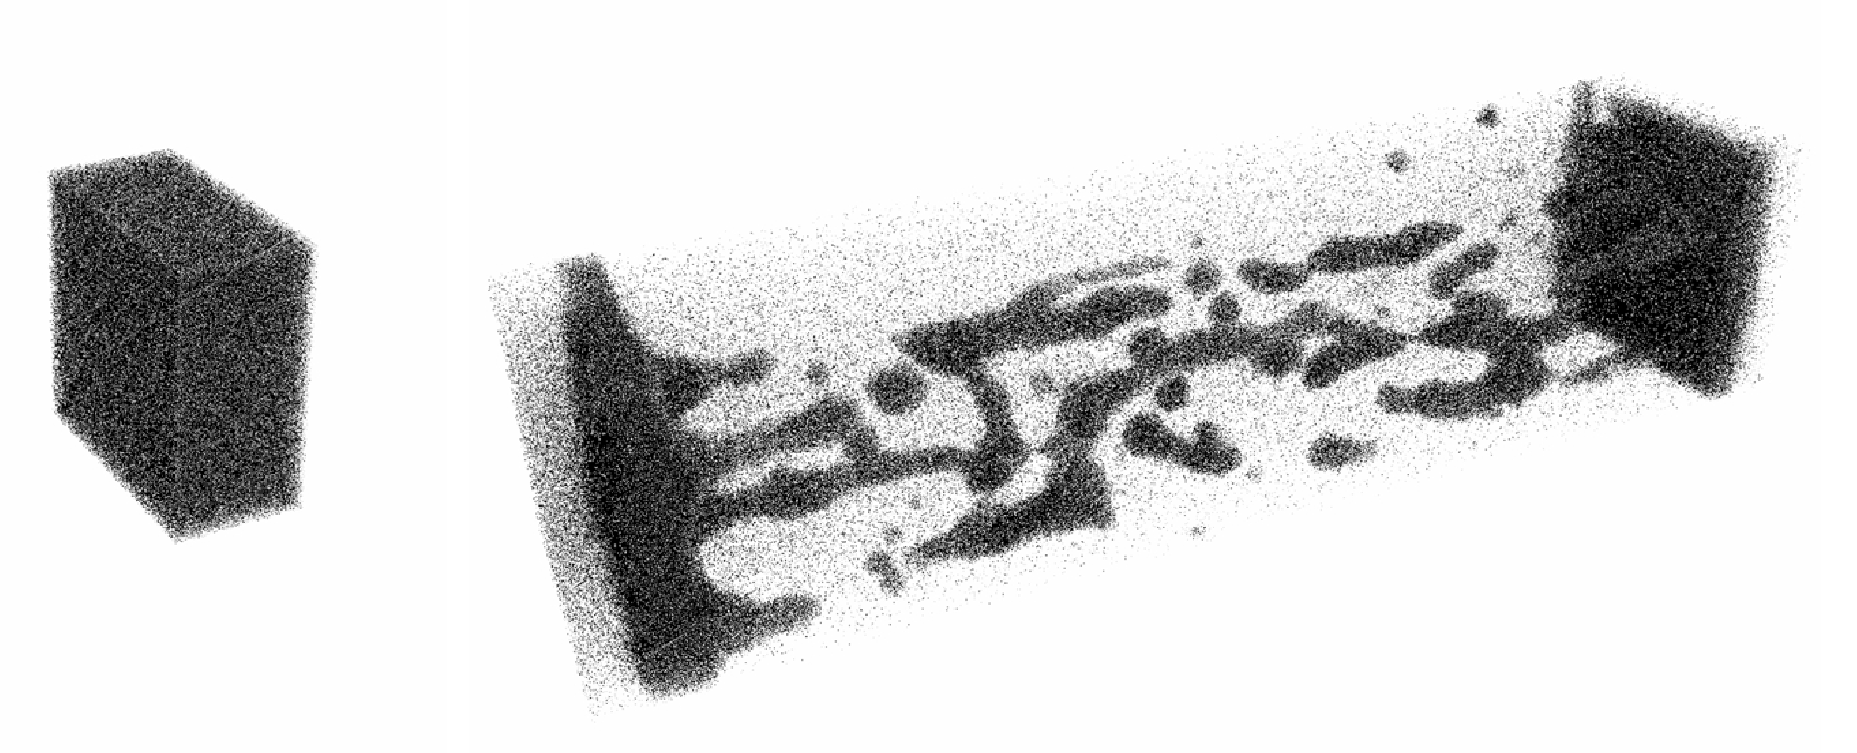
\includegraphics[width=0.9\linewidth]{imgs/explodingLiquid.png} % Dynamically scale the image
    \captionof{figure}{Exploding Liquid \parencite{seckler2021autopas}}
    \label{fig:exl}
\end{minipage}

\vspace{1em} % Optional vertical space between rows

\noindent
\begin{minipage}[t]{0.5\textwidth} % Reserve half a row for the third picture
    \centering
    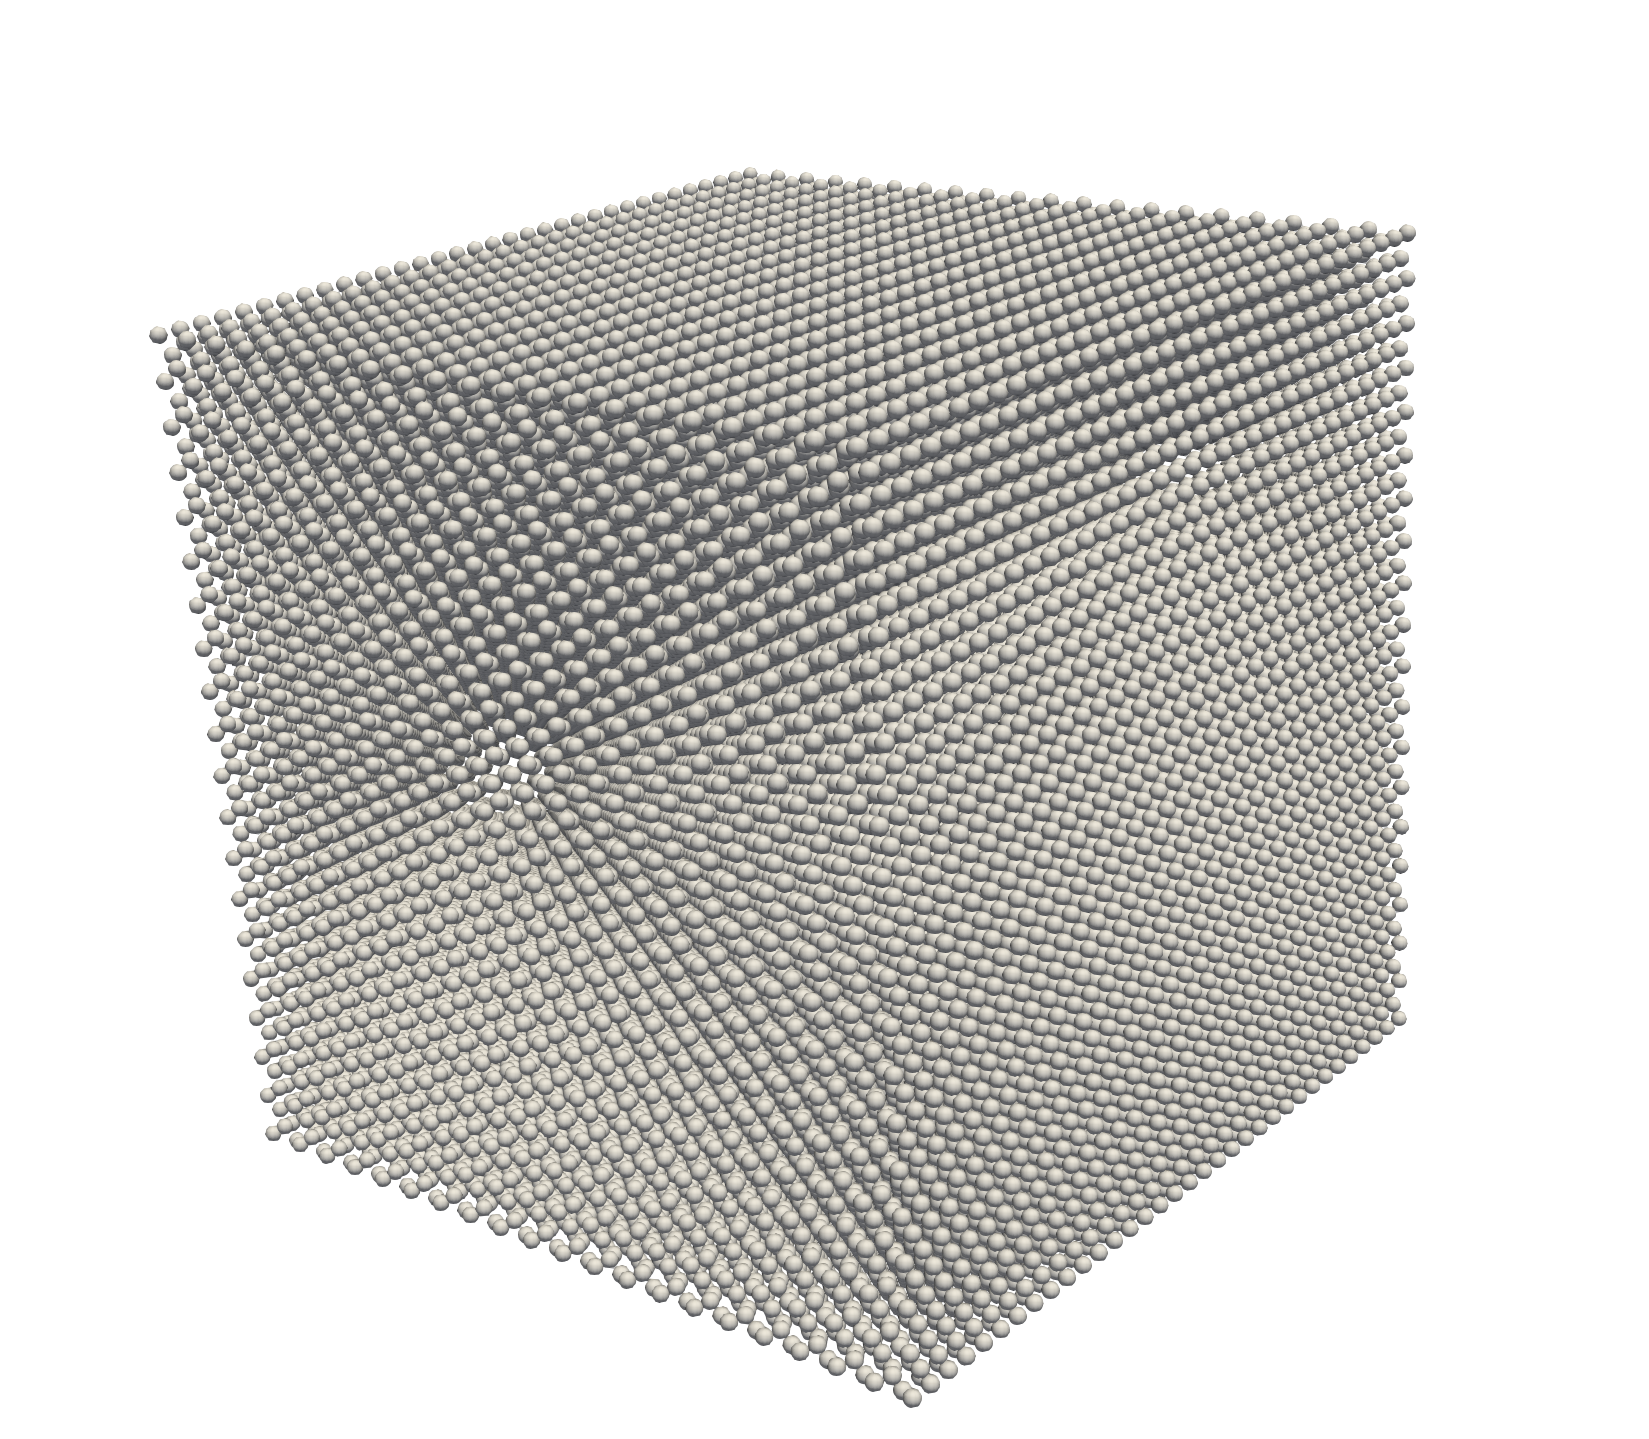
\includegraphics[width=0.5\linewidth]{imgs/constCube.png} % Dynamically scale the image
    \captionof{figure}{Constant Cube}
    \label{fig:conc}
\end{minipage}%
\begin{minipage}[t]{0.5\textwidth} % Reserve half a row for the fourth picture
    \centering
    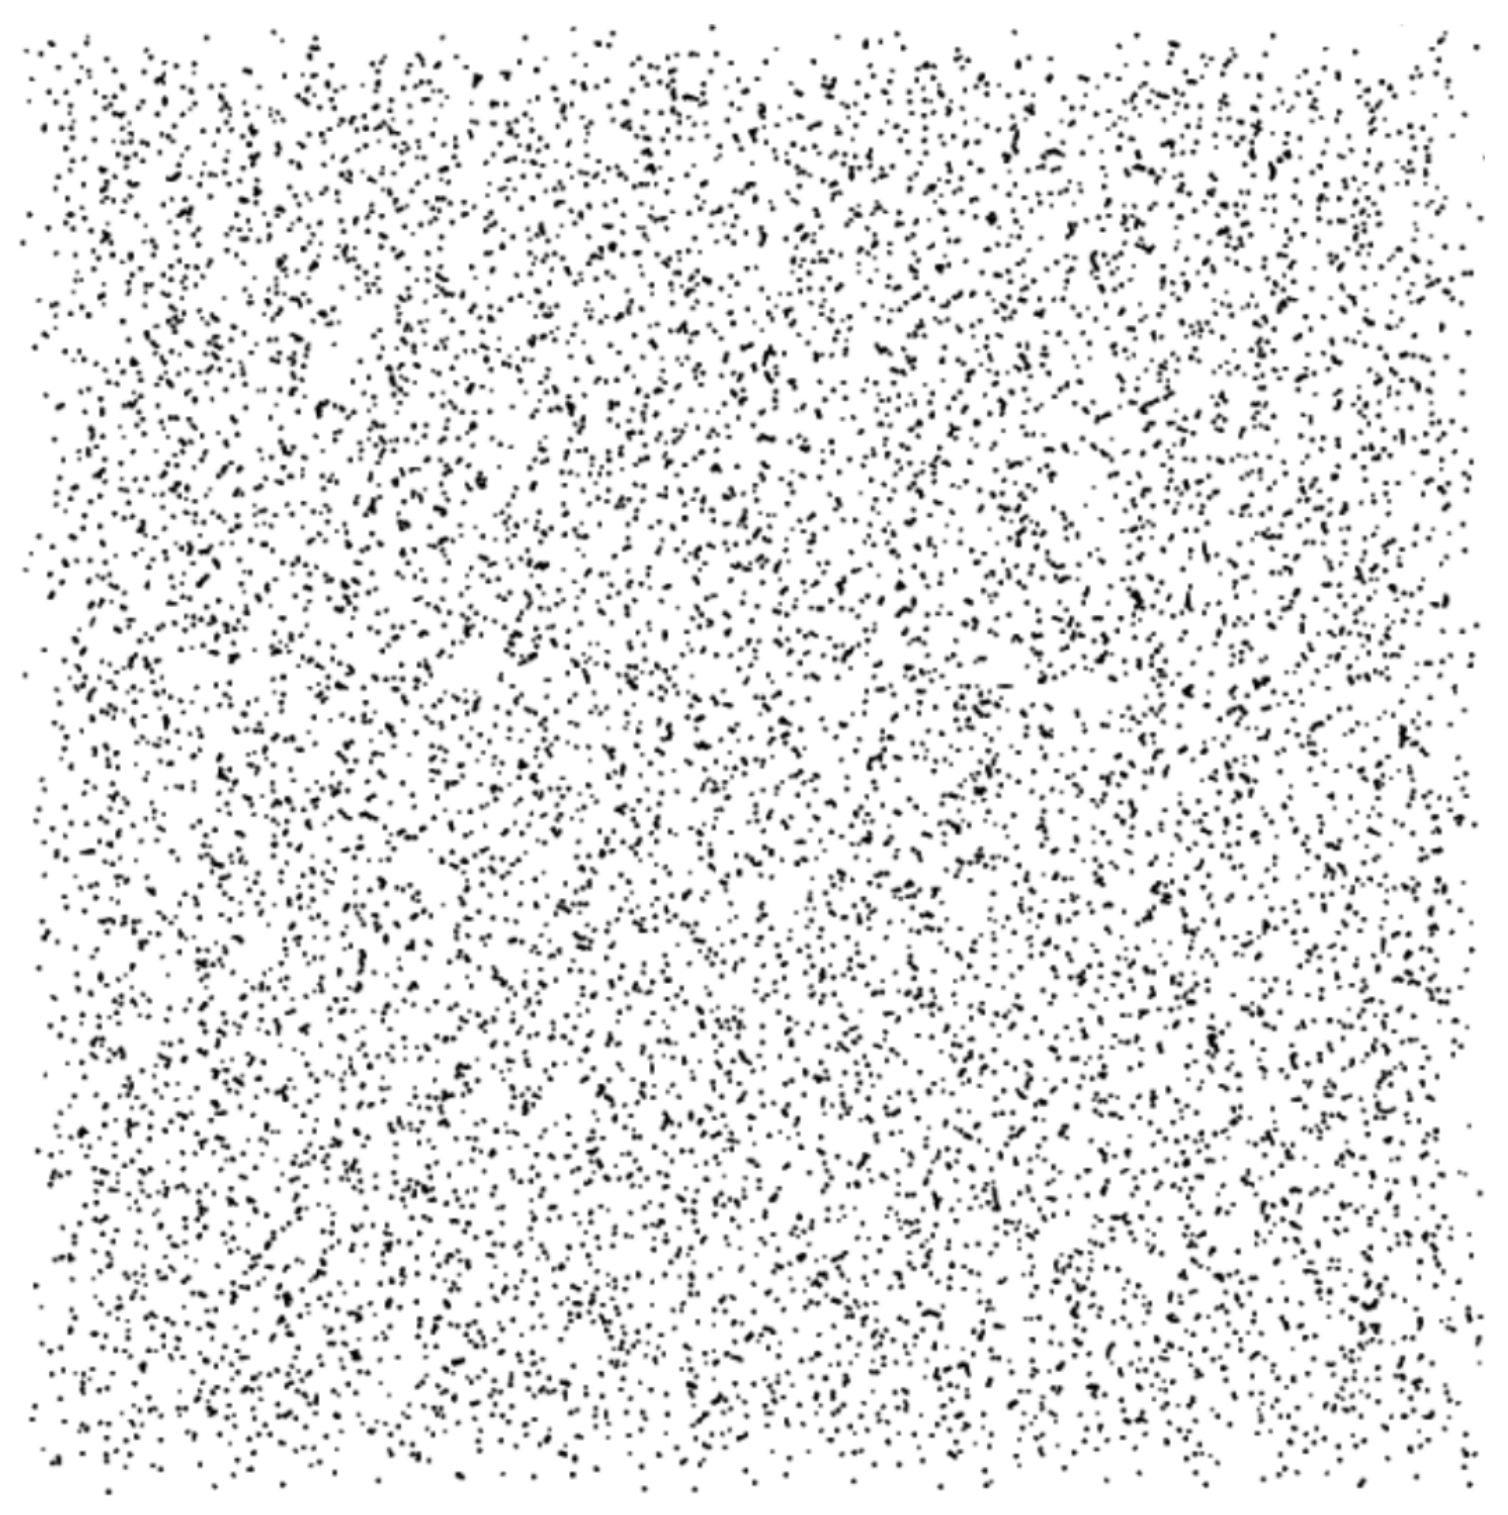
\includegraphics[width=0.5\linewidth]{imgs/spinodalDecomp.png} % Dynamically scale the image
    \captionof{figure}{Equilibration \parencite{Maximilian_Praus_Thesis-1.pdf}}
    \label{fig:equilibration}
\end{minipage}
\vspace{1em} 
\vspace{1em} 
\vspace{1em} 


% ======================================================================
\section{Experimental Strategies and Findings}


The primary objective was to evaluate the performance of the fast particle buffer by systematically modifying specific variables and observing its behavior across different scenarios. Additionally, the experiments aimed to assess the impact of these variables when applied in modified configurations of the same scenarios.

The variables selected for modification included:
\begin{itemize}
    \item \textbf{Verlet Rebuild Frequency}: This variable was adjusted to identify an optimal frequency that maximizes the reuse of neighbor lists across iterations without compromising runtime performance. The goal was to determine how much the rebuild frequency could be extended to achieve a performance gain.
    \item \textbf{Number of Particles}: The particle count was varied to analyze its influence on the buffer's efficiency, specifically examining whether smaller scenarios benefit from the buffer or if the improvements are primarily noticeable in larger configurations.
    \item \textbf{Iteration Count}: By increasing the number of iterations, the experiments aimed to evaluate whether extending the runtime reduces the need for frequent neighbor list rebuilds in scenarios where only a few fast particles remain after the dynamic phase.
\end{itemize}

The initial approach involved running a broad range of experiments, systematically varying these parameters to identify patterns and correlations. Key metrics of interest included the number of particles in the container versus the buffer and the time spent in \texttt{computeInteractions} compared to \texttt{remainderTraversal}. 
% The ultimate goal was to determine an ideal rebuild frequency and understand the relationship between these variables.

\subsection{Initial Test Series}

The initial series of experiments focused on analyzing frequency and iteration behavior across the first three scenarios.

\subsubsection{Frequency Tests}

Frequency tests were conducted by varying the rebuild frequency between 10 and 15,810. The objective was to evaluate the runtime behavior for typical low frequencies and higher frequencies exceeding the total number of iterations (effectively disabling rebuilds apart from tuning). A logarithmic distribution of frequencies was chosen to emphasize the analysis of larger frequencies. The following Python function illustrates the frequency selection logic:

\begin{lstlisting}[style=mypython]
def get_step_size(freq):
    log_freq = math.log10(freq)
    step_diff = max_step - min_step
    step_size = min_step + (log_freq * step_diff / math.log10(end_freq))
    return int(step_size)
\end{lstlisting}

For each frequency experiment, four types of graphs were generated to help interpret the results more effectively:

\begin{enumerate}
    \item A frequency vs. runtime graph comparing the performance of the parent branch \texttt{DynamicVLMerge} with the \texttt{Fast Particle Buffer} branch.
    \item A graph highlighting the differences in \texttt{computeInteractions} runtime between the two branches.
    \item A graph illustrating the differences in \texttt{remainderTraversal}.
\end{enumerate}

The results consistently showed that the fast particle buffer performed worse across all scenarios and frequencies:
\begin{itemize}
    \item For the Falling Drop scenario, the runtime ranged from 1.1 to 6 times slower. \ref{fig:tuningfallingDrop}
    \item For the Exploding Liquid scenario, the runtime ranged from 1.1 to 4 times slower. \ref{fig:tuningexplodingLiquid}
    \item For the Constant Velocity Cube scenario, the runtime ranged from 1.3 to 11.2 times slower. \ref{fig:tuningconstantVelocityCube}
\end{itemize}

To investigate the cause of this performance degradation, the focus was shifted to analyzing the graphs highlighting computeInteractions and remainderTraversal. However, these graphs were challenging to interpret due to significant spikes caused by the tuning phase. Tuning is the most computationally expensive part of the simulation, and its periodic spikes (determined by the tuning frequency) overshadowed the subtler runtime variations, making it difficult to analyze the true behavior of the buffer.


% \begin{figure}[htbp]
%     \centering
%     \vspace{-0.5em}
%     \begin{subfigure}[b]{\textwidth}
%         \centering
%         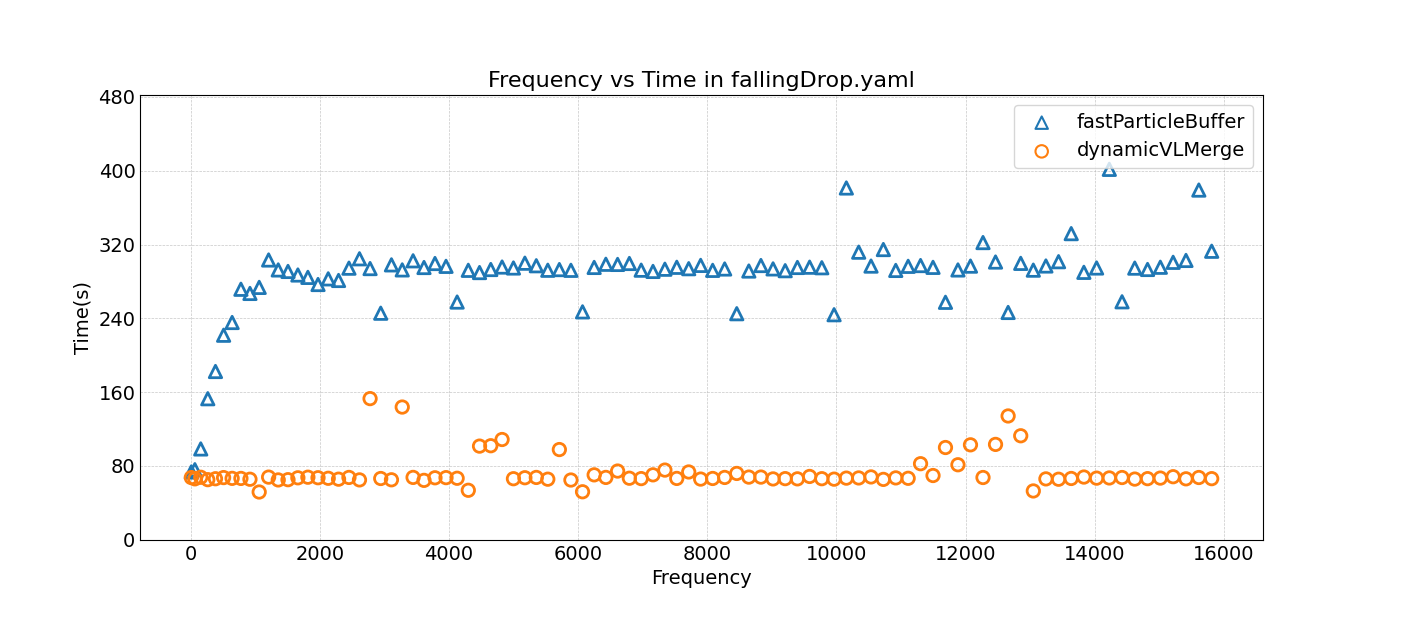
\includegraphics[width=0.9\linewidth]{graphs/fallingDrop/freqvstime.png}
%         \vspace{-0.5em}
%         \caption{\scriptsize Falling Drop}
%         \label{fig:tuningfallingDrop}
%     \end{subfigure}

%     \begin{subfigure}[b]{\textwidth}
%         \centering
%         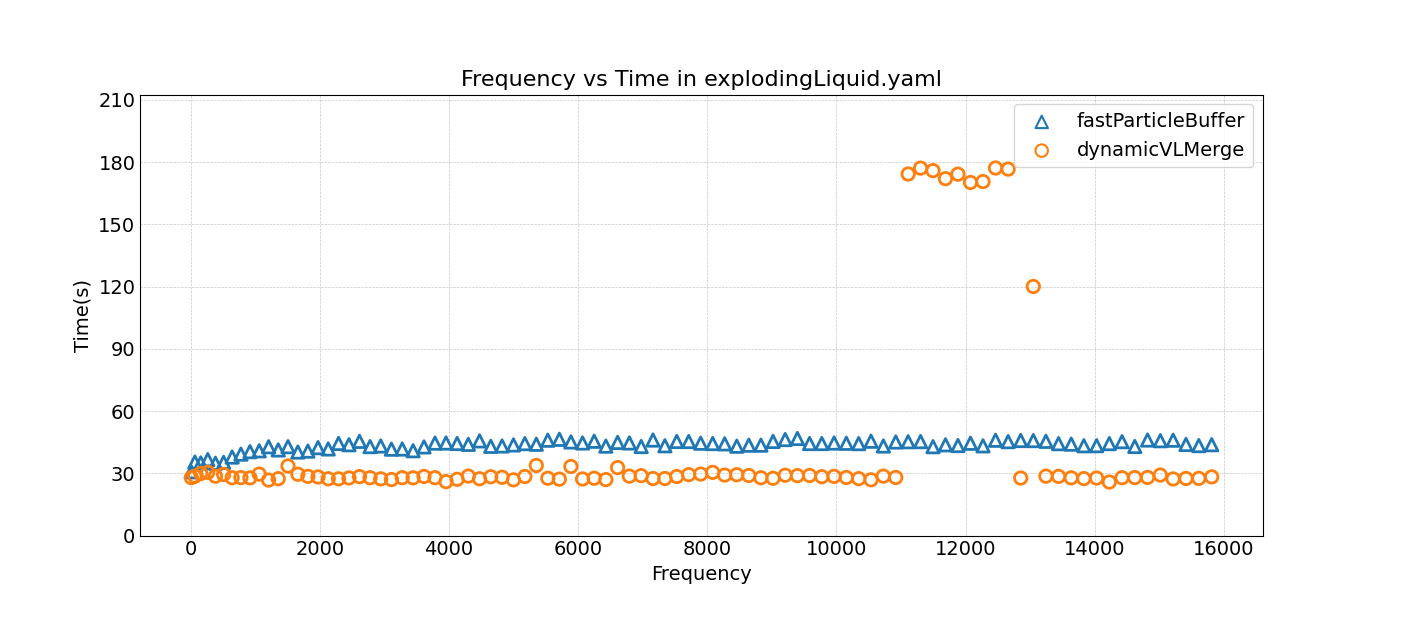
\includegraphics[width=0.9\linewidth]{graphs/explodingLiquid/freqvstime.png}
%         \vspace{-0.5em}
%         \caption{\scriptsize Exploding Liquid}
%         \label{fig:tuningexplodingLiquid}
%     \end{subfigure}

%     \begin{subfigure}[b]{\textwidth}
%         \centering
%         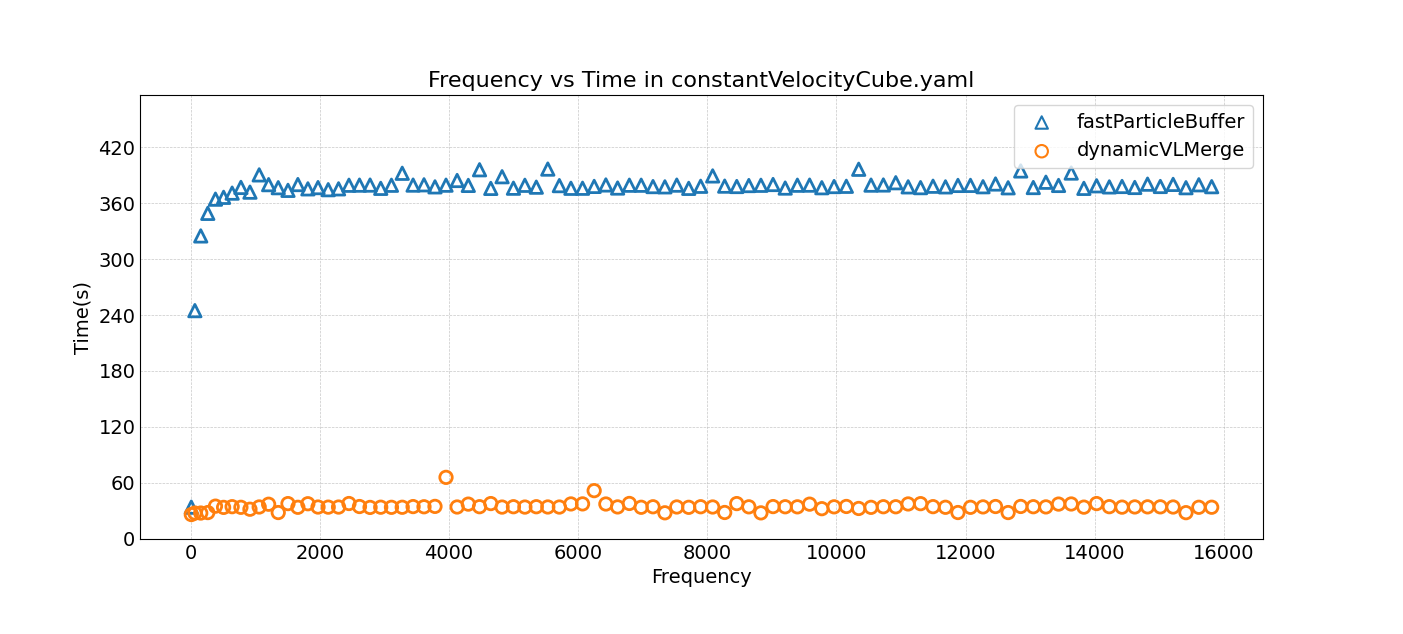
\includegraphics[width=0.9\linewidth]{graphs/constantVelocityCube/freqvstime.png}
%         \vspace{-0.5em}
%         \caption{\scriptsize Constant Velocity Cube}
%         \label{fig:tuningconstantVelocityCube}
%     \end{subfigure}

%     \vspace{1em}
%     \caption{Comparison of Frequency vs Time with Tuning}
%     \label{fig:main}
% \end{figure}



\subsubsection{Refined Tests Without Tuning Spikes}

To better understand the program's behavior, the tuning phase was effectively eliminated by specifying exact configurations for the container and traversal. This ensured that the simulation used fixed setups without requiring tuning. Since testing all possible configurations was impractical, three key traversal-container combinations were selected:


\begin{itemize}
    \item \textbf{Traversal}: \texttt{vlc\_c08 / vlp\_c08}, \textbf{Container}: VerletListsCells, \textbf{Data Layout}: AoS, \\ \textbf{Newton3}: Enabled
    \item \textbf{Traversal}: \texttt{vcl\_c06}, \textbf{Container}: VerletClusterLists, \textbf{Data Layout}: AoS, \\ \textbf{Newton3}: Enabled
    \item \textbf{Traversal}: \texttt{lc\_c08}, \textbf{Container}: LinkedCellsReferences, \textbf{Data Layout}: SoA, \\ \textbf{Newton3}: Enabled
\end{itemize}



Frequency tests were then repeated for the first three scenarios using these fixed configurations. This approach eliminated tuning-related noise, allowing for a clearer analysis of how the buffer performed under different traversal and container setups. By isolating these configurations, it was possible to focus on the individual behaviors of each traversal and container, leading to more thorough insights into the implementation's performance.

Upon examining the individual frequency versus time graphs that compare the different configurations across various scenarios (Figures \ref{fig:mainFallingDrop} \ref{fig:mainExplodingLiquid} \ref{fig:mainConstantVelocityCube}), the implementation with the fast particle buffer generally underperformed relative to the implementation without it.

A unique case, however, is observed at frequency 10, where the Fast-Particle-Buffer branch performs nearly as well as the parent branch. This behavior occurs because, at such a low frequency, there are almost no fast particles; the neighbor lists are rebuilt so frequently that particles do not have sufficient time to accumulate in the buffer. 


\paragraph{Falling Drop:}

The runtime of the Fast-Particle-Buffer branch across all configurations was up to four times longer than that of the parent branch, Dynamic-VL-Merge (see Figure \ref{fig:mainFallingDrop}). This raises the question: what is the underlying cause of this difference in performance? 

To investigate, we focus on the relationship between  compute interactions, remainder traversal (Fig.\ref{fig:vlcc08inter156}), and neighbor list rebuild times per iteration (Fig.\ref{fig:vlcc08_neighbour_156}), as well as the number of particles stored in the buffer per iteration (Fig.\ref{fig:vlcc08_buffer_size_156}).



\begin{figure}[htbp]
    \centering
    % \vspace{-0.5em}
    % \begin{subfigure}[b]{\textwidth}
        % \centering
        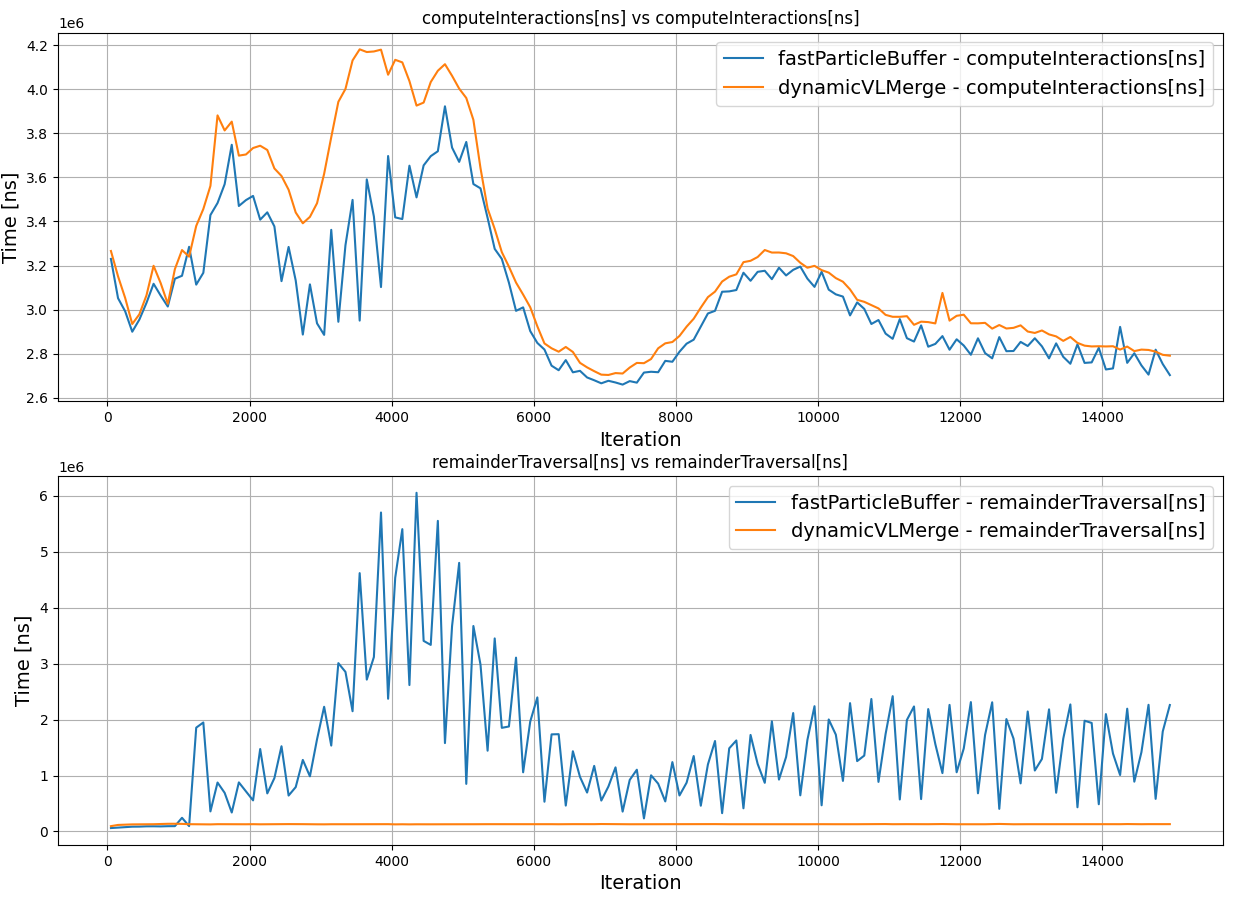
\includegraphics[width=0.9\linewidth]{graphs/fallingDrop/normalExperiments/freq/vlcc08inter156.png}
        \vspace{-0.5em}
        \caption{Compute interactions versus Remainder traversal Falling Drop Vlc\_c08}
        \label{fig:vlcc08inter156}
\end{figure}

\begin{figure}[htbp]
    \centering
    % \vspace{-0.5em}
    % \begin{subfigure}[b]{\textwidth}
        % \centering
        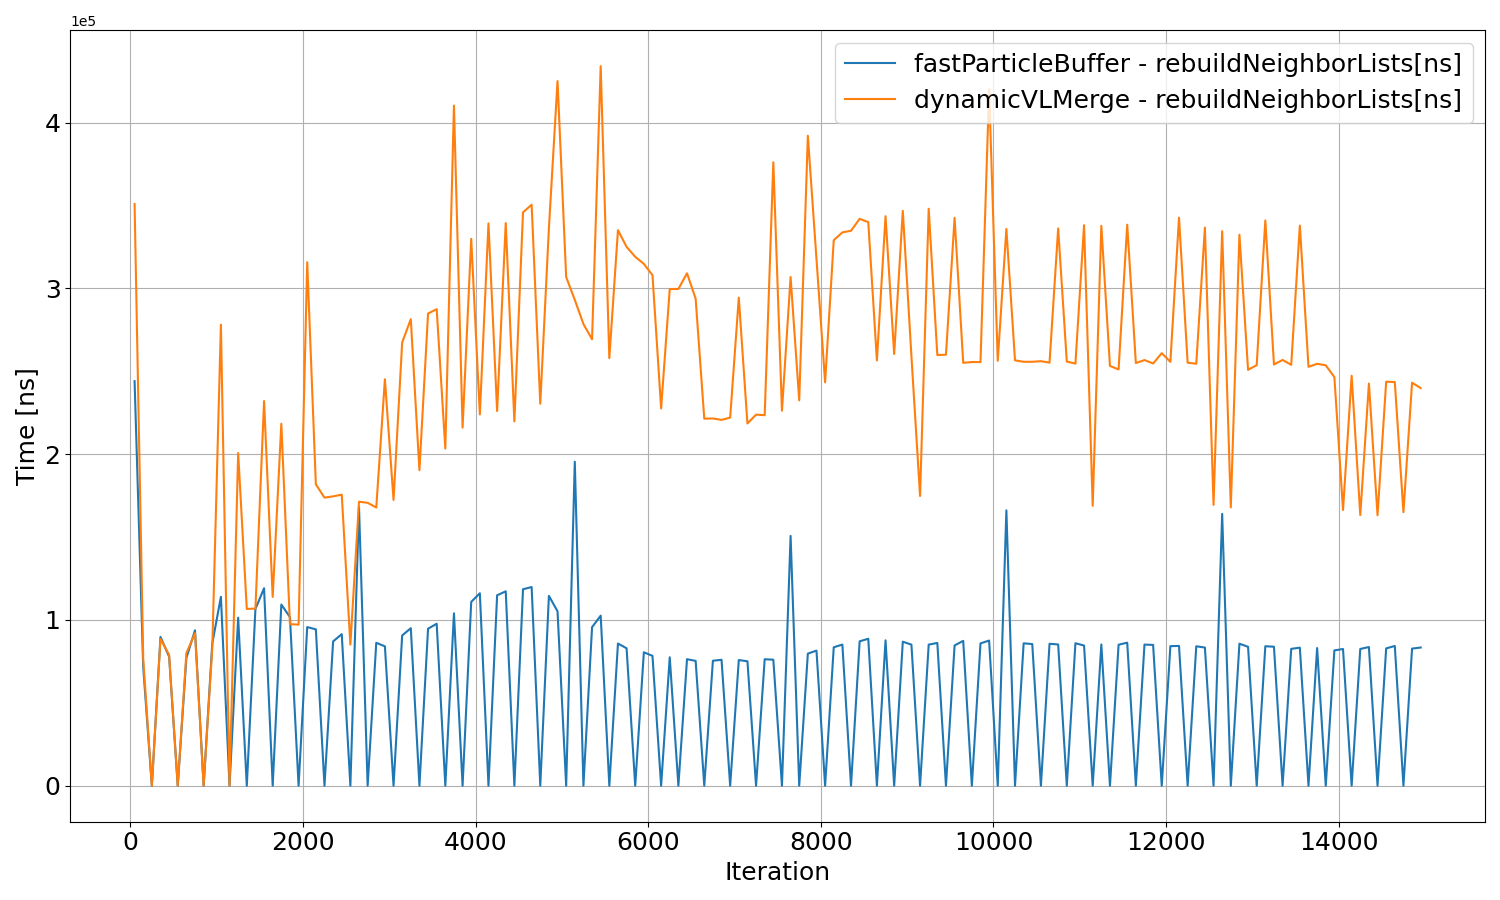
\includegraphics[width=0.9\linewidth]{graphs/fallingDrop/normalExperiments/freq/vlcc08_neighbour_156.png}
        \vspace{-0.5em}
        \caption{Time spent rebuilding neighbor lists in Falling Drop Vlc\_c08}
        \label{fig:vlcc08_neighbour_156}
\end{figure}

\begin{figure}[htbp]
    \centering
    % \vspace{-0.5em}
    % \begin{subfigure}[b]{\textwidth}
        % \centering
        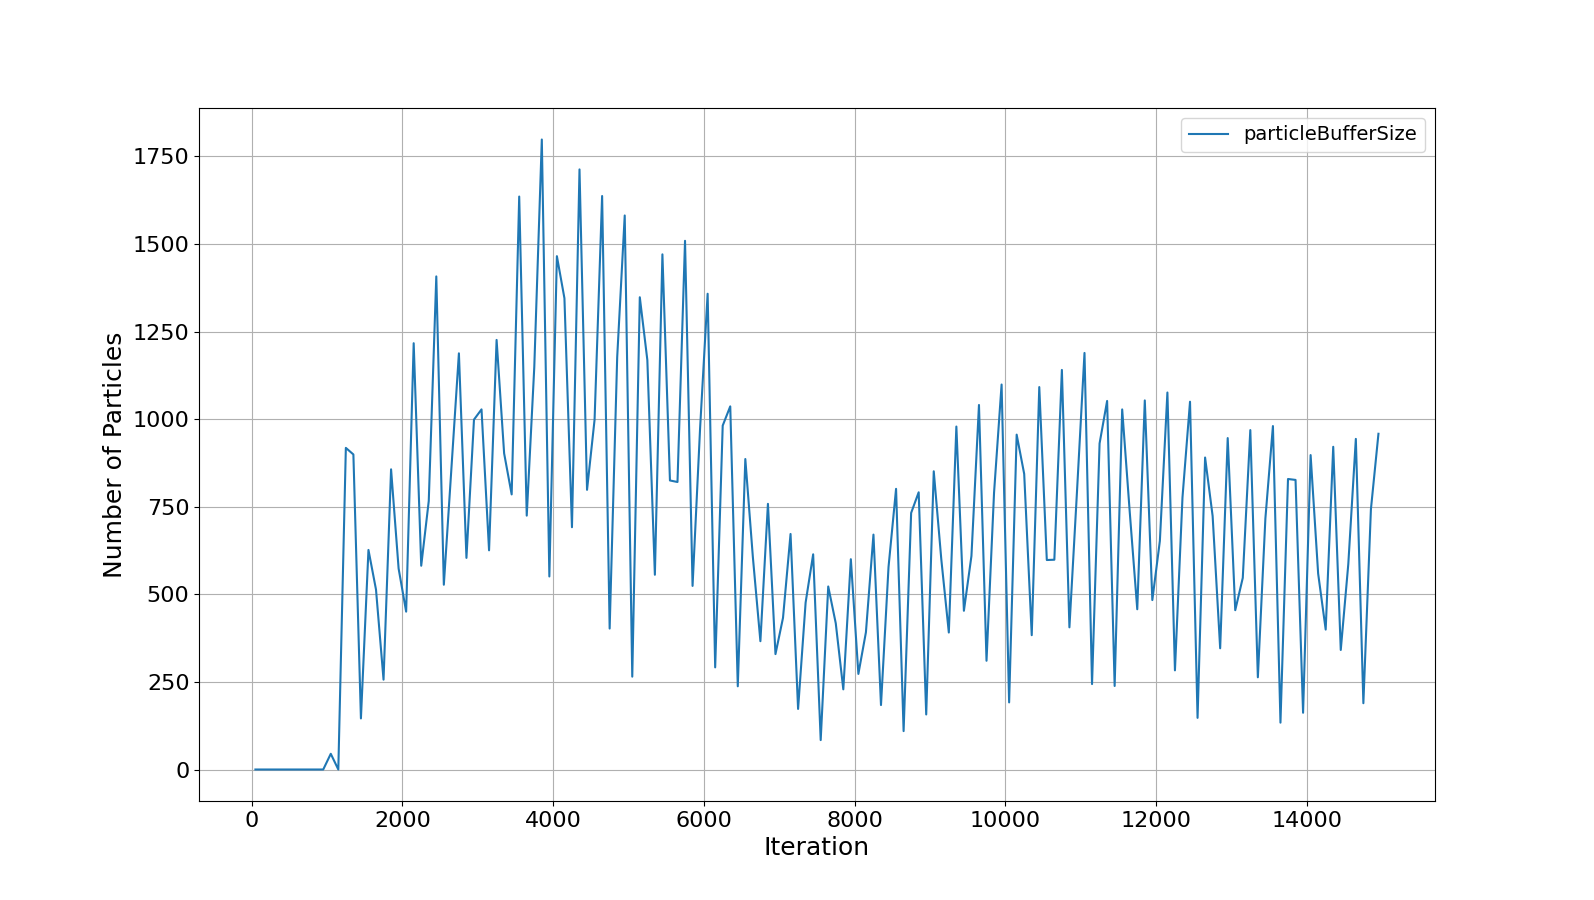
\includegraphics[width=\linewidth]{graphs/fallingDrop/normalExperiments/freq/vlcc08_buffer_size_156.png}
        \vspace{-0.5em}

        \caption{Buffer Size throughout Iterations in Falling Drop Vlc\_c08}
        \label{fig:vlcc08_buffer_size_156}
\end{figure}



Between iterations 2000 and 5000, there is a gradual accumulation of particles in the buffer, peaking at approximately 1798 particles around iteration 3850. Following this peak, the number of particles in the buffer starts to decline. This fluctuation is directly reflected in the remainder traversal time, which increases as the buffer fills up and decreases once particles start leaving the buffer. 

While there is a reduction in the time spent on \texttt{computeInteractions} within the Fast-Particle-Buffer branch (due to particles being removed from the container), this saving is overshadowed by the significant increase in the time required for remainder traversal calculations. At its peak, the remainder traversal phase in the Fast-Particle-Buffer branch takes more time than the \texttt{computeInteractions} phase itself in the Dynamic-VL-Merge branch, where all particles are being considered. 

One noticeable advantage of the Fast-Particle-Buffer approach is the reduction in neighbor list rebuild time, which takes an average four times less time compared to the Dynamic-VL-Merge branch (Fig.\ref{fig:vlcc08_neighbour_156}). However, the saved time does not compensate for the excessive time spent in remainder traversal. The combined savings from both reduced \texttt{computeInteractions} and neighbor list rebuilds are significantly smaller than the additional time required for remainder traversal.

At the end of the experiment, the recorded execution times for key operations in both branches are as follows:

\begin{itemize}
    \item \textbf{Fast-Particle-Buffer:}
    \begin{itemize}
        \item \texttt{computeInteractions[ns]}: $45.74$ s
        \item \texttt{remainderTraversal[ns]}: $23.40$ s
        \item \texttt{rebuildNeighborLists[ns]}: $0.92$ s
    \end{itemize}
    \item \textbf{Dynamic-VL-Merge:}
    \begin{itemize}
        \item \texttt{computeInteractions[ns]}: $48.23$ s
        \item \texttt{remainderTraversal[ns]}: $1.95$ s
        \item \texttt{rebuildNeighborLists[ns]}: $3.73$ s
    \end{itemize}
\end{itemize}

The higher the frequency, the more time is saved from avoiding neighbor list rebuilds. However, the rate at which remainder traversal time increases significantly outweighs the benefits. To illustrate, at frequency 15,810 (where rebuilding no longer occurs, as all particles are in the buffer), the theoretical maximum time savings from avoiding rebuilds is approximately $3.5 \times 10^5$ ns per iteration. However, the average remainder traversal time per iteration reaches approximately $1.38 \times 10^7$ ns, demonstrating that the overhead introduced by the buffer is vastly greater than the savings obtained from eliminating neighbor list rebuilds.

\paragraph{Constant Velocity Cube:}

The Constant Velocity Cube scenario exhibited similar behavior, where the fast particle buffer consistently underperformed compared to the counterpart (Fig. \ref{fig:mainConstantVelocityCube}). Performance differences ranged from:
\begin{itemize}
    \item 6 times slower for \texttt{vlp\_c08} (selected instead of \texttt{vlc\_c08}, as \texttt{vlp\_c08} was frequently chosen during tuning experiments due to its optimization for this scenario).
    \item Up to 18 times slower for \texttt{lc\_c08}.
    \item Approximately 4 times slower for \texttt{vcl\_c06}.
\end{itemize}

The reasoning for these results remains consistent: the time saved from infrequent neighbor list rebuilds is outweighed by the excessive computation time in remainder traversals.

\paragraph{Exploding Liquid:}
In the Exploding Liquid scenario, the traversals \texttt{lc\_c08} and \texttt{vlc\_c08} demonstrated similar performance trends to those observed in other scenarios (Fig. \ref{fig:mainExplodingLiquid}). However, an exception was noted in the \texttt{vcl\_c06} (Fig.\ref{fig:vclc06explodingLiquid}) traversal. During this traversal, the Dynamic VL Merge branch exhibited an average runtime nearly twice as long as the other two traversals, whereas the runtime of the Fast-Particle-Buffer branch increased only slightly in comparison.

Analyzing frequencies between 10 and 2451, the Fast-Particle-Buffer branch outperformed the Dynamic VL Merge branch. The shortest runtime achieved by the Fast-Particle-Buffer branch was 37.88 seconds at frequency 265, whereas the lowest runtime for the Dynamic VL Merge branch within \texttt{vcl\_c06} was 39.2 seconds in iteration 9963. 


A deeper analysis of the \texttt{computeInteractions} and \texttt{remainderTraversal} times provides insight into the underlying reason for this speedup. Unlike in other traversals, \texttt{computeInteractions} in the parent branch consumed significantly more time using \texttt{vcl\_c06}, whereas the remainder traversal time in the Fast-Particle-Buffer branch experienced changes that were not as drastic (Fig. \ref{fig:mainexplodingLiquid_inter}). This discrepancy led to a unique case where the increased computational cost of \texttt{computeInteractions} in the Dynamic VL Merge branch effectively offset the additional remainder traversal time in the Fast-Particle-Buffer branch. Consequently, for \texttt{vcl\_c06}, the Fast-Particle-Buffer branch gained a net advantage by reducing the cost of neighbor list rebuilds.

However, while this might initially appear as a speedup, it is important to put the results into context. The lowest overall runtime across all traversal methods was not achieved by the Fast-Particle-Buffer branch but rather by the Dynamic VL Merge branch in other traversal configurations. This suggests that, although the Fast-Particle-Buffer branch outperformed the Dynamic VL Merge branch specifically for \texttt{vcl\_c06}, it was not the most efficient approach across all tested traversal methods. Therefore, while the buffer mechanism provided a performance gain in this isolated case, it did not lead to an overall improvement in execution time across the entire experiment.




\subsubsection{Iteration Tests}


For the iteration tests, a base frequency of 100 was maintained for the first two scenarios and 1000 for the third scenario. The number of iterations varied between 500 and 30,000, with a step size of 500 iterations. The goal of these experiments was to observe the behavior of fast particles at different stages of the simulation by increasing the number of iterations. This approach aimed to identify any correlations between simulation progression and the performance of the particle buffer implementation, as well as to expand the range of experiments conducted.

Initially, as in the frequency tests, the first three scenarios were executed with tuning enabled. However, this did not provide sufficient insight into the performance of the fast particle branch. The results of these initial tests are presented in the appendix [\textbf{link appendix}].

\subsubsection{Individual Test Results}

\textbf{Falling Drop Scenario:}
For the \texttt{vlc\_c08} traversal, no performance improvement was observed. Across all iteration counts, the fast particle buffer consistently performed worse than the Dynamic VL Merge branch. 

The same trend was observed for \texttt{lc\_c08}. The remainder traversal phase required excessive time, negating any potential gains from avoiding neighbor list rebuilds. Thus, the time saved from fewer rebuilds was insufficient to offset the overhead introduced by the remainder traversal.

[\textbf{Note: Include \texttt{computeInteractions} graphs for \texttt{vcl\_c08} and \texttt{vcl\_c06}}]

In contrast, the \texttt{vcl\_c06} traversal demonstrated similar performance for both branches. In some cases, the fast particle buffer was 1--2 seconds faster. This can be explained by the runtime differences visible in the graphs below.  For \texttt{vcl\_c06}, \texttt{computeInteractions} required nearly four times more runtime than \texttt{vcl\_c08} (note the difference in scales: \texttt{vcl\_c06} has an ordinate axis in $e7$, while \texttt{vcl\_c08} is in $e6$). However, the remainder traversal times were comparable between the two. This outcome arises because the fast particle buffer, implemented as a vector of vectors, is not influenced by the container or traversal type. Despite the improved results in this specific experiment, no significant overall performance improvement was observed. Note that these graphs use a window average of 100 to reduce noise.

% \begin{center}
% 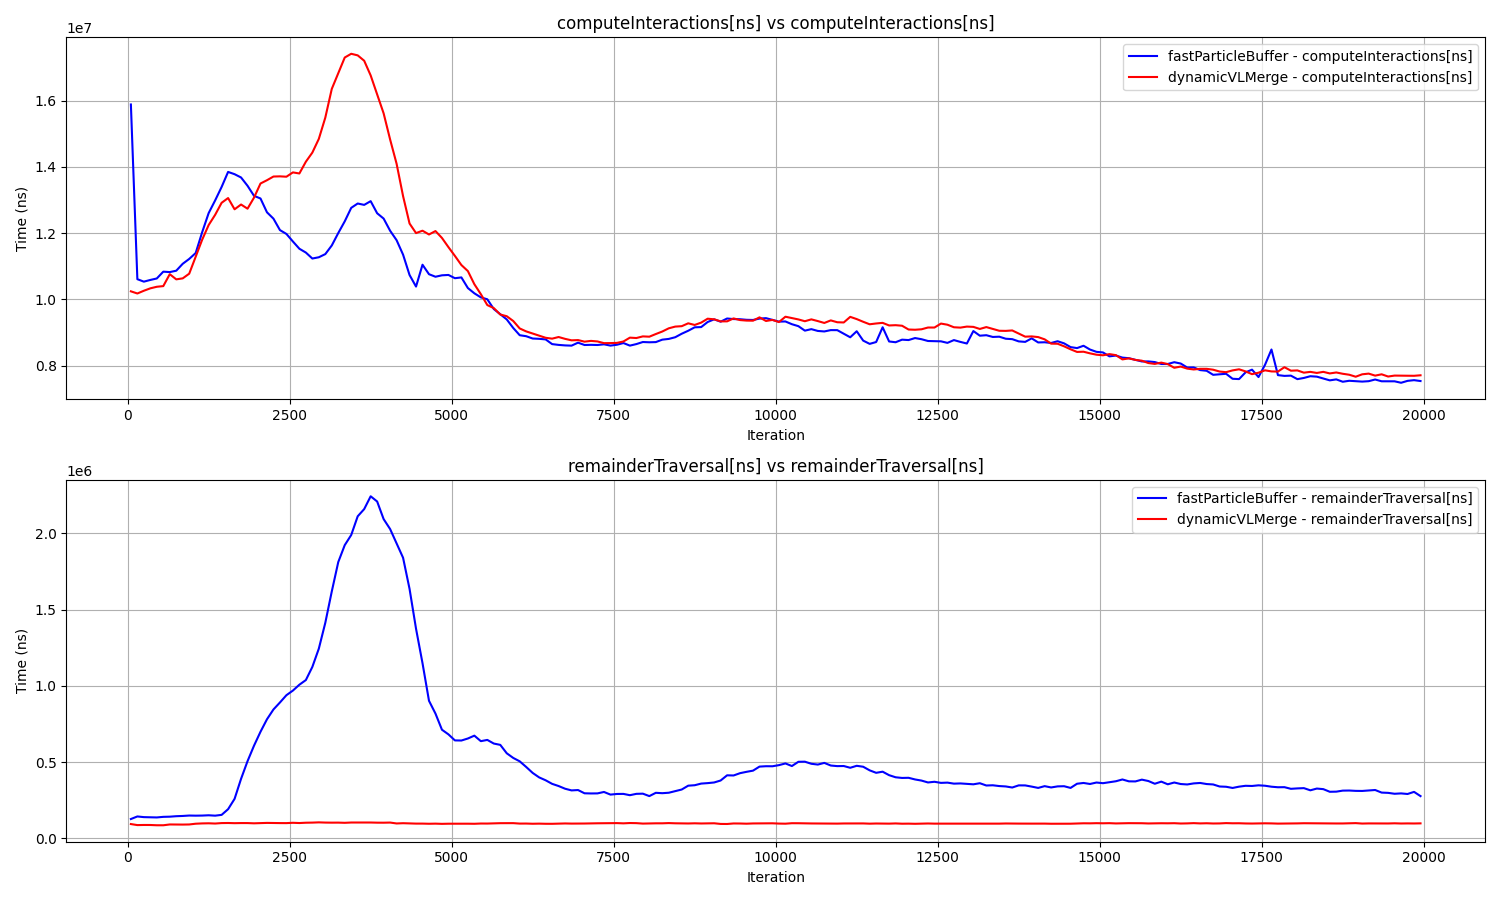
\includegraphics[width=\linewidth]{graphs/fallingDrop/normalExperiments/iter/vclc06dvlfp.png}
% \vspace{-0.4em}
% \captionof{figure}{Compute Interactions and Remainder Traversal in Falling Drop \texttt{vcl\_c06}.}
% \vspace{-0.4em}
% 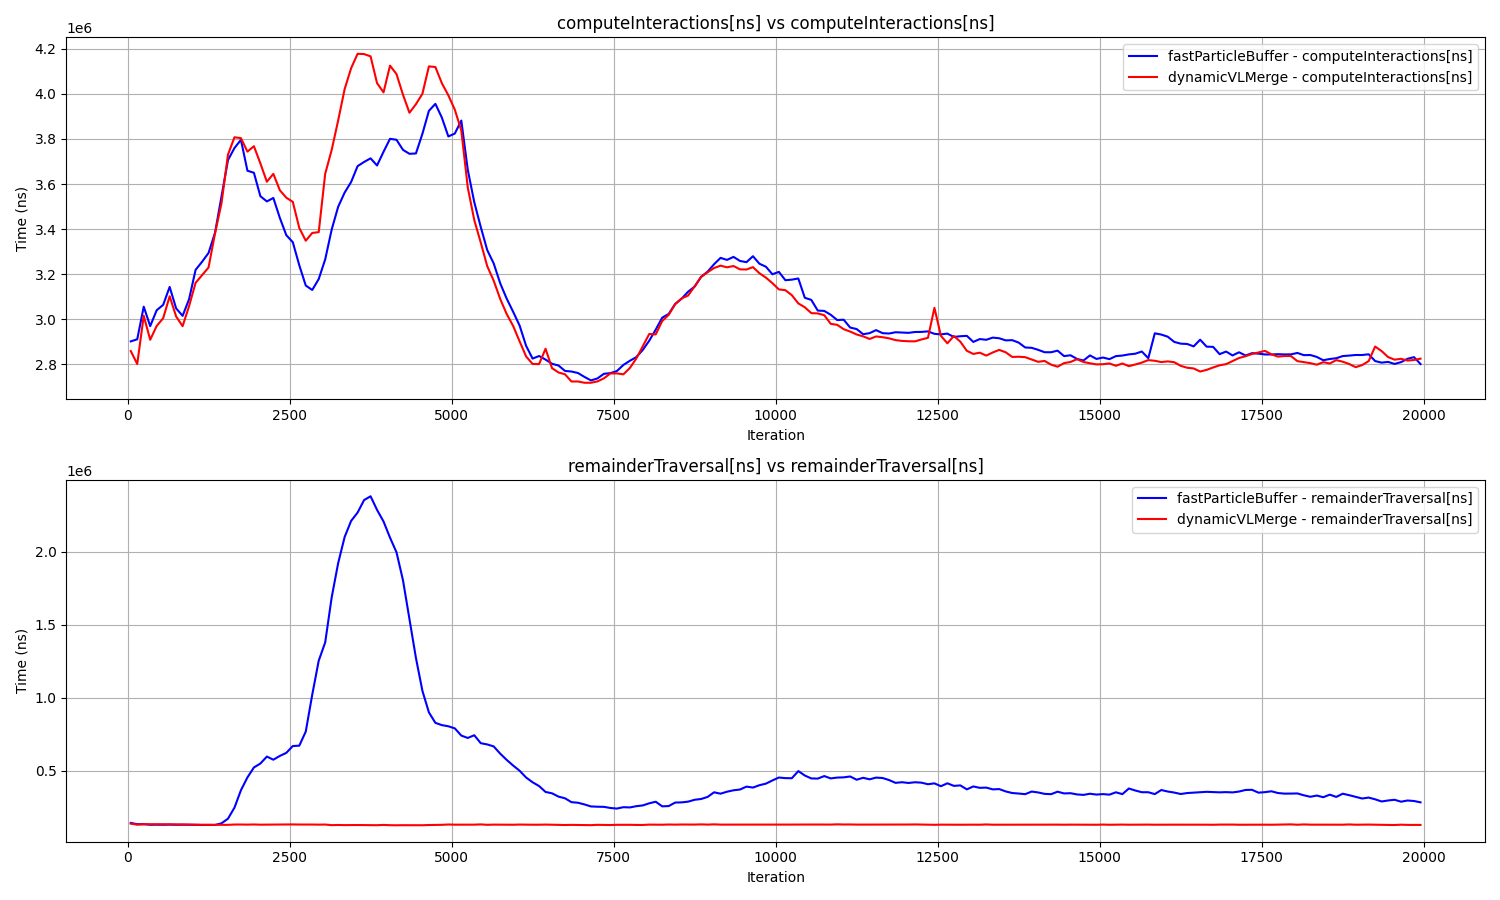
\includegraphics[width=\linewidth]{graphs/fallingDrop/normalExperiments/iter/vlc08dvlfp.png}
% \vspace{-0.4em}
% \captionof{figure}{Compute Interactions and Remainder Traversal in Falling Drop \texttt{vlc\_c08}.}
% \vspace{-0.4em}
% \end{center}

\begin{center}
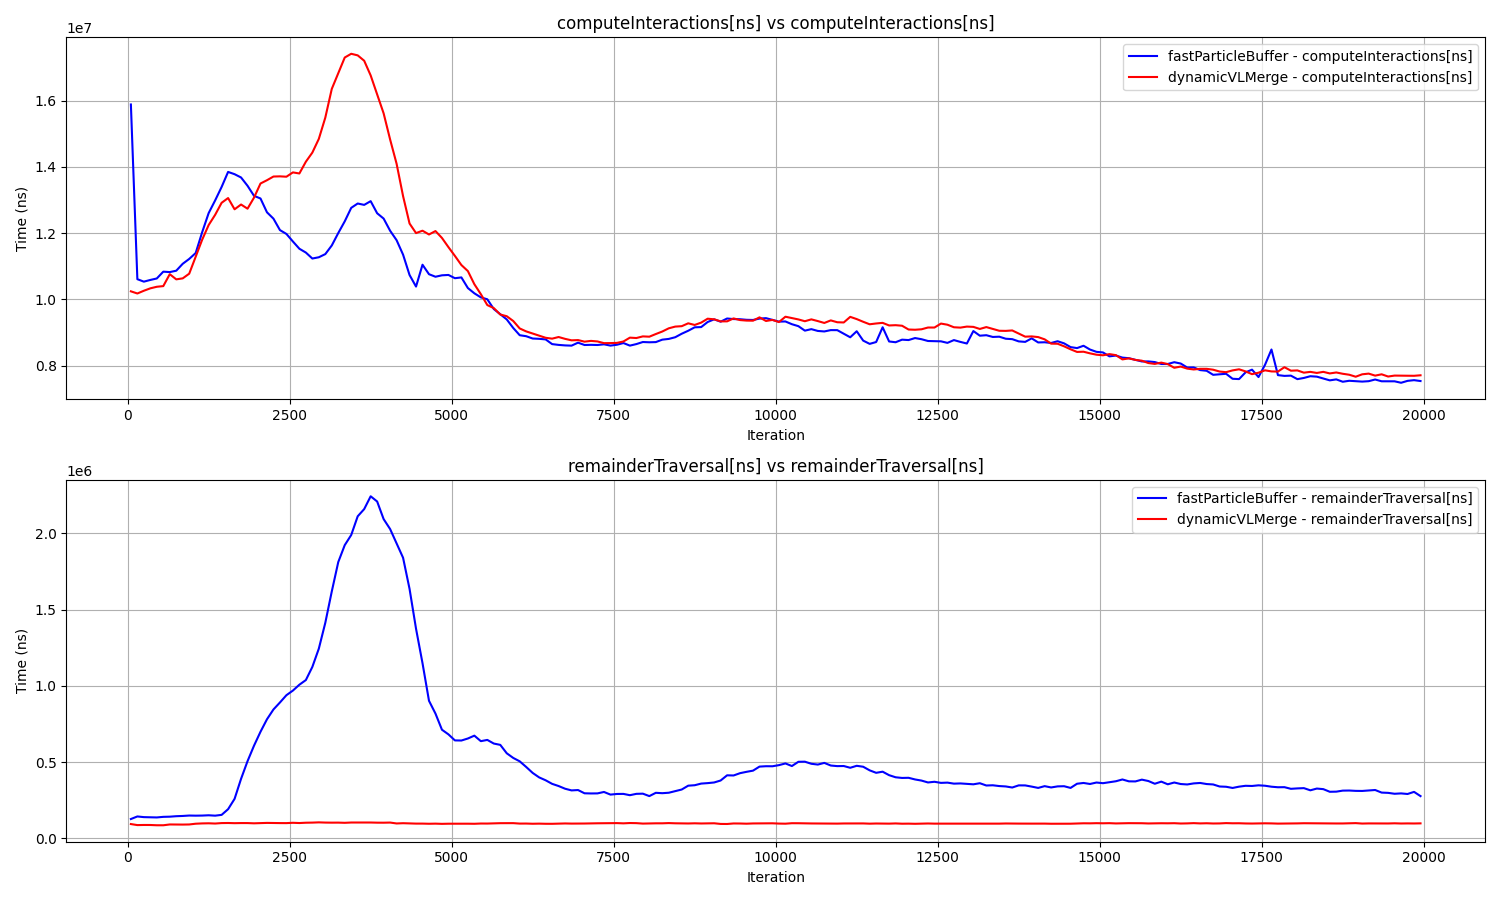
\includegraphics[width=\linewidth]{graphs/fallingDrop/normalExperiments/iter/vclc06dvlfp.png}
\captionof{figure}{Compute Interactions and Remainder Traversal in falling drop vclc06}
\end{center}

\begin{center}
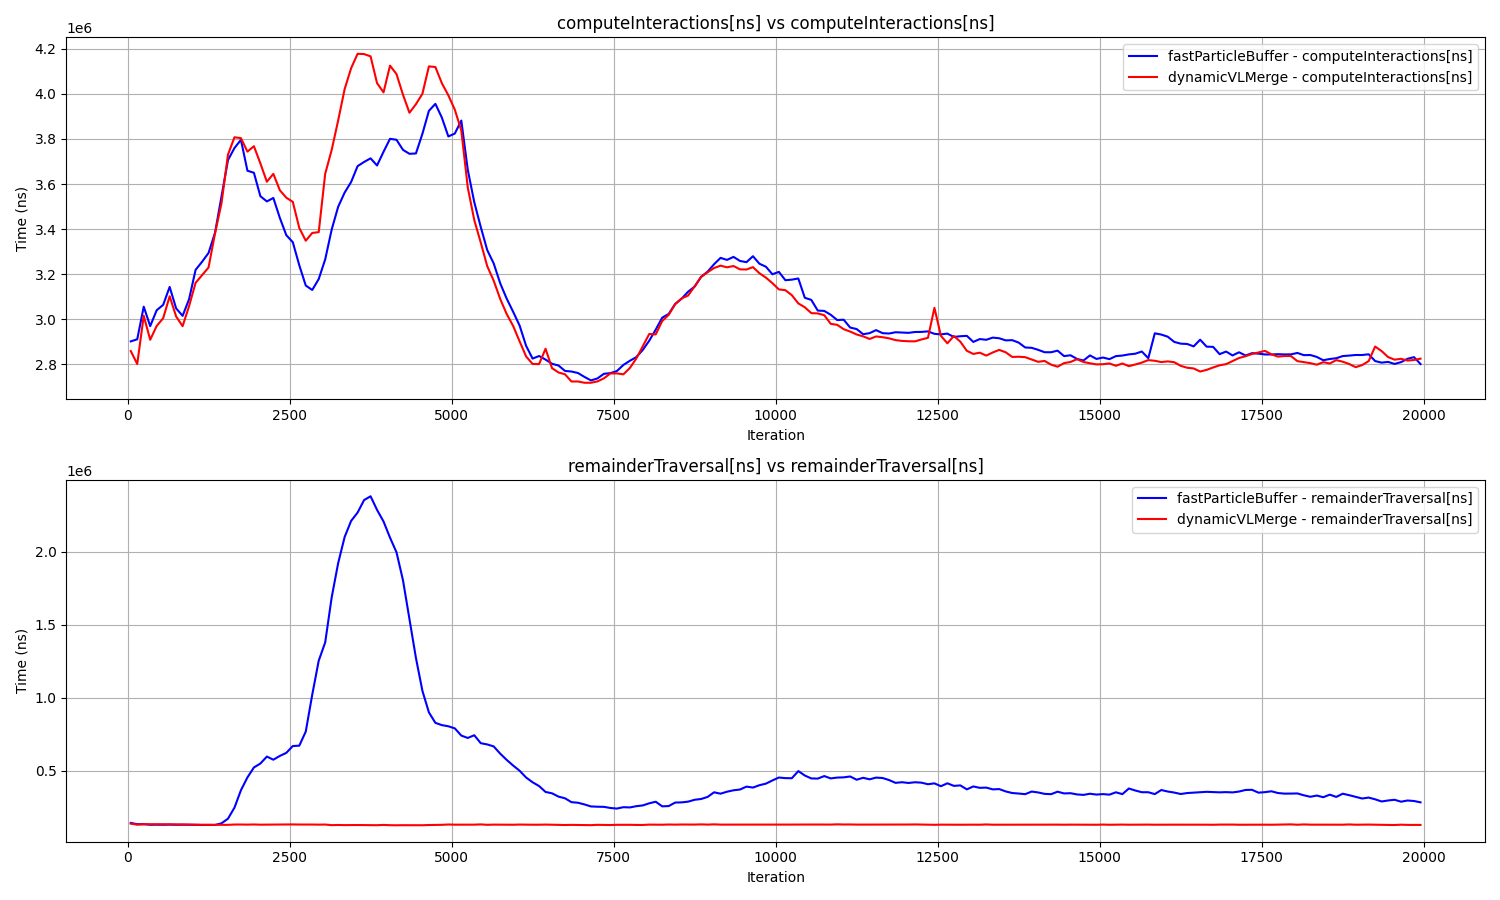
\includegraphics[width=\linewidth]{graphs/fallingDrop/normalExperiments/iter/vlc08dvlfp.png}
\captionof{figure}{Compute Interactions and Remainder Traversal in falling drop vlcc08}
\end{center}

\textbf{Exploding Liquid Scenario:}
The results for this scenario followed a pattern similar to Falling Drop. The performance trends of the traversals were comparable between the two scenarios. However, anomalies were observed in the behavior of \texttt{vlc\_c08} and \texttt{vcl\_c06}, as indicated in the graphs [\textbf{link Exploding Liquid graphs}]. Missing lines in the graphs suggest that the experiment failed for certain iteration counts in both branches. Although there were spikes in \texttt{vlc\_c08}, where the fast particle buffer branch appeared to outperform the Dynamic VL Merge, the anomalies in the experiments render these results unreliable. Since both branches failed under certain conditions, these results cannot be considered valid. The \texttt{lc\_c08} traversal, however, exhibited stable behavior with no failed runs.

\textbf{Constant Velocity Cube Scenario:}
In this scenario, no performance improvement was observed for the fast particle buffer. Instead, the performance difference between the two branches was more pronounced compared to Falling Drop. For \texttt{lc\_c08}, the fast particle buffer was up to 16 times slower; for \texttt{vcl\_c06}, it was 4 times slower; and for \texttt{vlp\_c08}, it was around 3 times slower. [\textbf{Why is the performance so poor? Adjust the reasoning for choosing Constant Velocity Cube, as there is still significant particle interaction.}]

This poor performance is due to the large number of particles accumulating in the buffer. For instance, in the experiment with 30,000 iterations, more than half of the total particles—around 28,000 out of 50,000—were in the buffer. This high number of particles in the buffer significantly increased the time required for remainder traversal. In the graph below, the runtime scale for remainder traversal is $e8$, while \texttt{computeInteractions} is on the $e7$ scale, showing a clear difference in time consumption.

The issue lies in the difference in optimization between the buffer and the container. Containers and traversals are designed to be efficient and parallelized, allowing particles to be processed quickly. In contrast, the fast particle buffer is a simple vector of vectors and is not optimized in the same way, leading to much higher computation times for remainder traversal when many particles are stored in the buffer.

\begin{center}
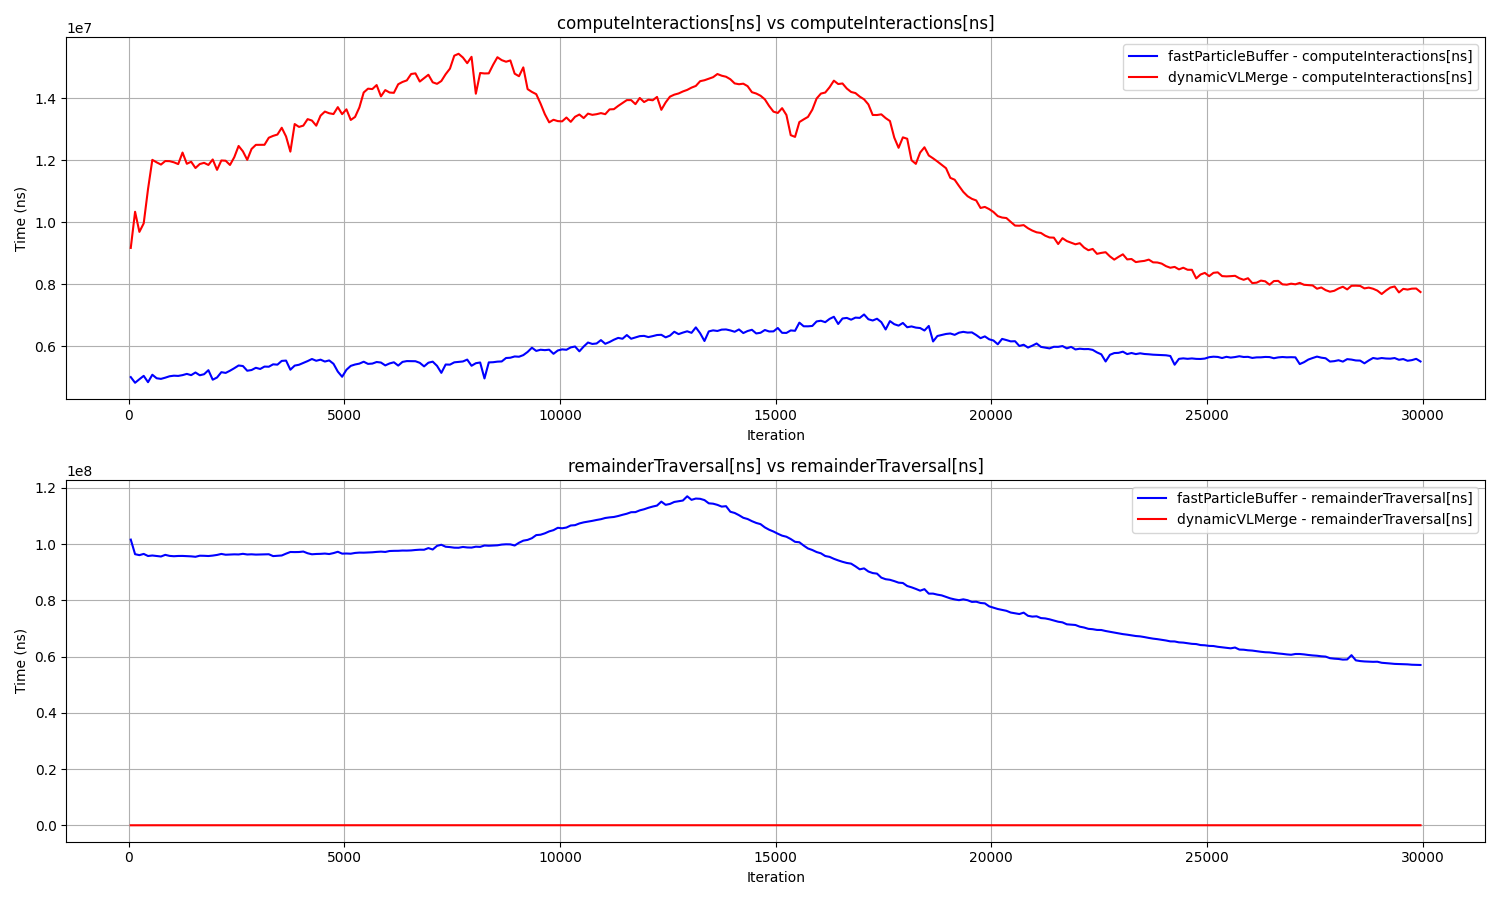
\includegraphics[width=\linewidth]{graphs/constantVelocityCube/normalExperiments/iter/vlpc08dvlpb.png}
\captionof{figure}{Compute Interactions and Remainder Traversal in Constant Velocity Cube \texttt{vlp\_c08}.}
\end{center}


% \clearpage
\begin{figure}[htbp]
    \centering
    
    \begin{subfigure}[b]{\textwidth}
        \centering
        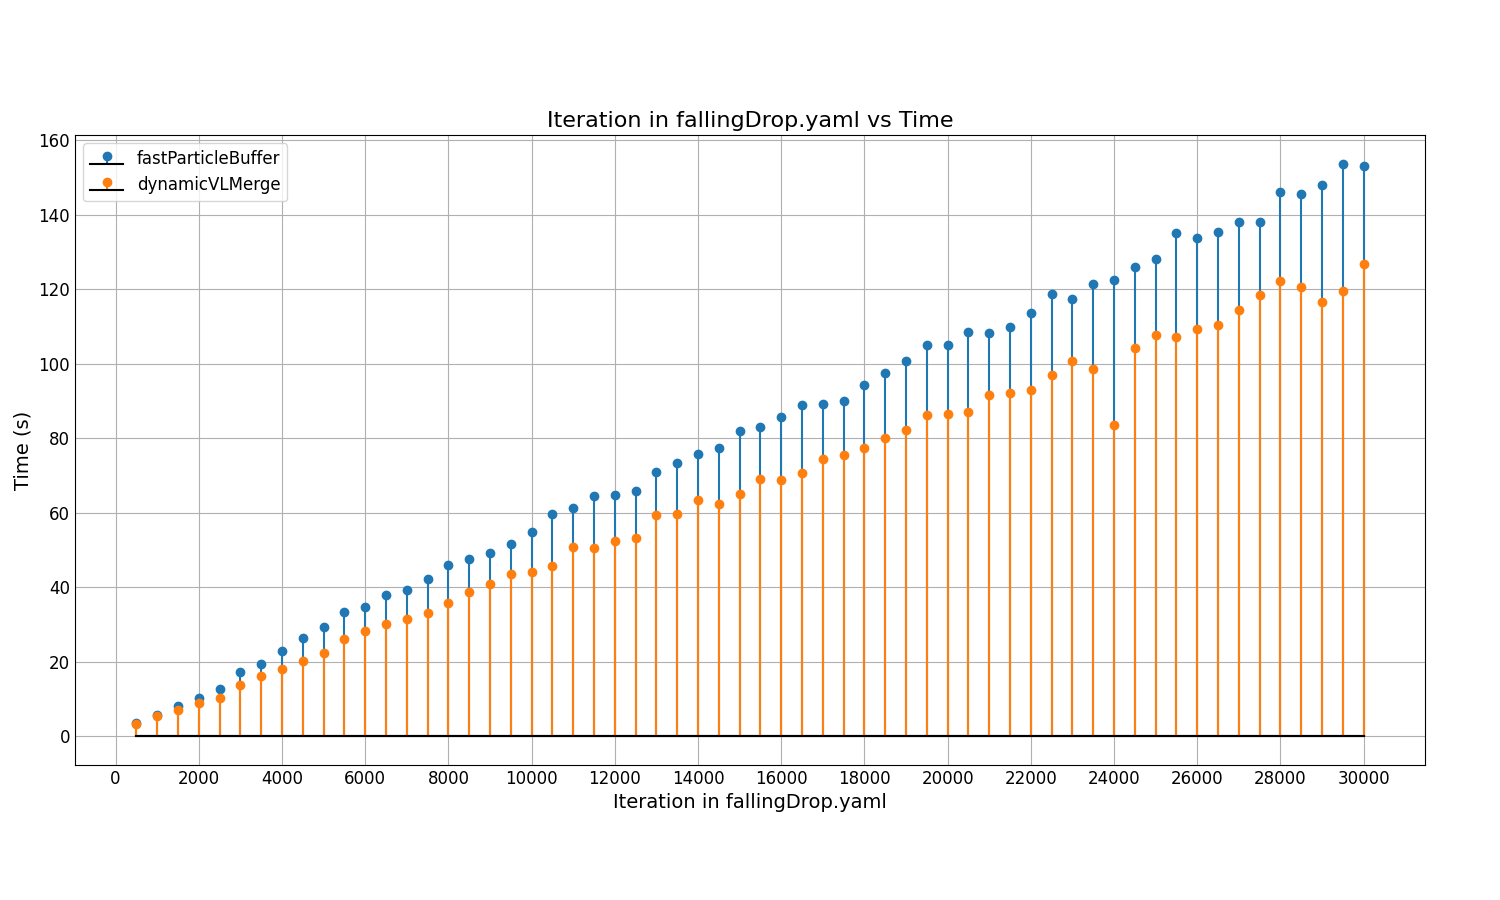
\includegraphics[width=0.6\textwidth]{graphs/fallingDrop/freqvstimeiter.png}
        \caption{\scriptsize Frequency vs Time for Falling Drop}
        \label{fig:fallingDrop}
    \end{subfigure}

    \begin{subfigure}[b]{\textwidth}
        \centering
        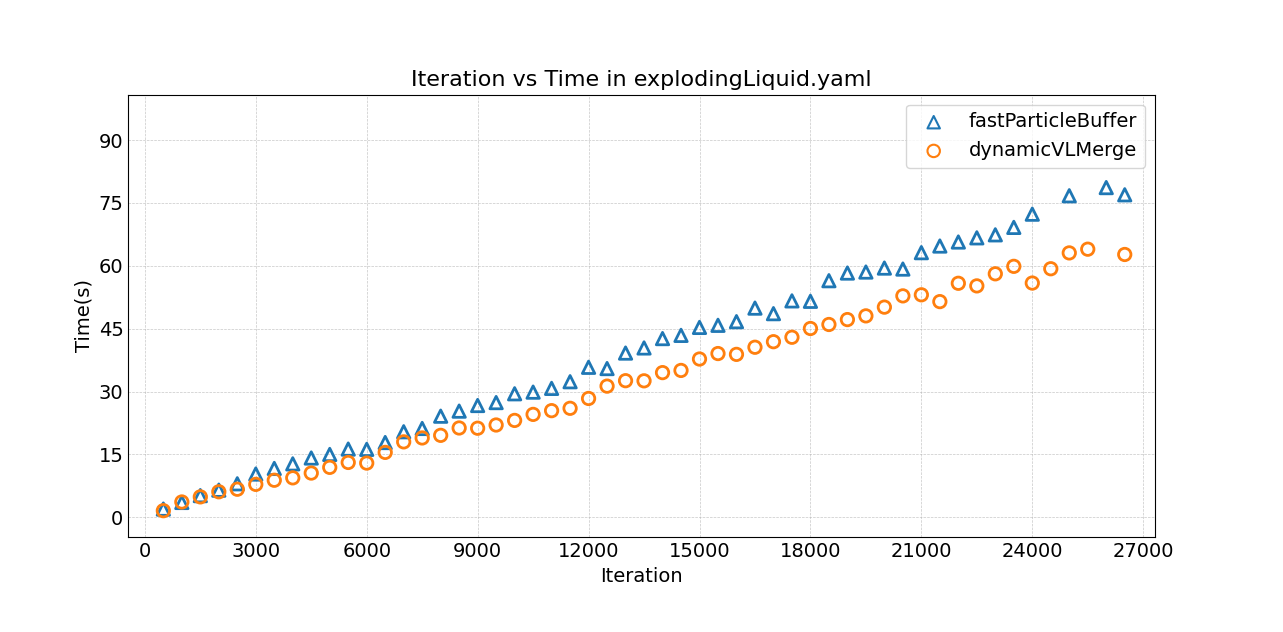
\includegraphics[width=0.6\textwidth]{graphs/explodingLiquid/freqvstimeiter.png}
        \caption{\scriptsize Frequency vs Time for Exploding Liquid}
        \label{fig:explodingLiquid}
    \end{subfigure}

    \begin{subfigure}[b]{\textwidth}
        \centering
        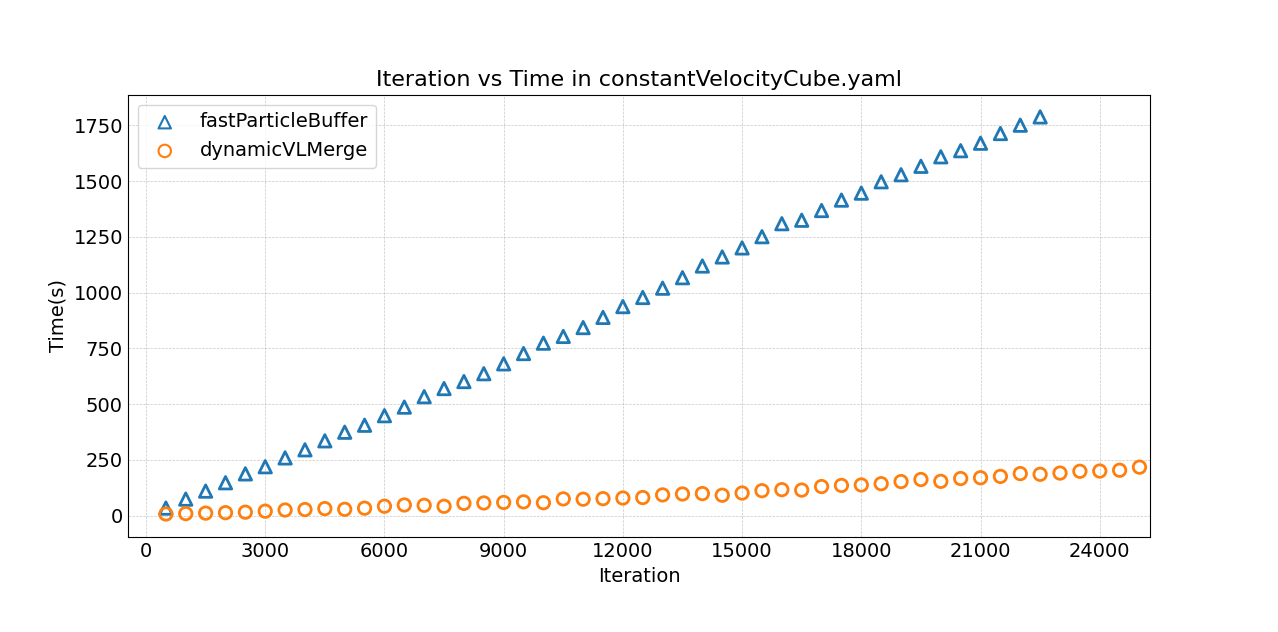
\includegraphics[width=0.6\textwidth]{graphs/constantVelocityCube/freqvstimeiter.png}
        \caption{\scriptsize Frequency vs Time for Constant Velocity Cube}
        \label{fig:constantVelocityCube}
    \end{subfigure}

    \caption{Comparison of Frequency vs Time for Different Simulations}
    \label{fig:main}
\end{figure}



% percentage expr
%     - why only run in some of them
%     - why still not performat
%     - why chose to use spinodal all of a sudden 
%     - idea to converge to DVL
%     - is the slight improvement only a coincidence - repeating the tests many times
%     - idea to increase the temperatur in spinodial decomp 
% Profiler
% add where to find the tests on github and such, also attach slurm job maybe

\subsection{Percentage Experiments}

% Since the problem with the fast particle implemntation was that the remainder traversal takes significantly more time than the time saved from not doing the neighbor rebuilds so often, the idea was to decrease the number of particles that can gather in the buffer to a percentage of the total amount of the particles in the buffer, so that we ll have less particle to iterate through in the buffer, but still save neighbor lists rebuild time.  



\subsection{Spinodal Decomposition Equilibration}

Given that the observed performance speedup in earlier experiments ranged between only 1 to 2 seconds, it raises the question of whether these results were merely coincidental or indicative of actual improvement. To address this, percentage-based experiments were conducted for the fourth scenario, spinodal decomposition equilibration. The hypothesis was that, due to the highly dynamic nature of this scenario and its substantial number of particles (4 million), there would be noticeable performance improvements when using the particle buffer.

From prior frequency experiments, it was observed that the particle buffer performed better at smaller frequencies. Therefore, this experiment focused on frequencies ranging from 10 to 50 with a step size of 10. Additionally, as established earlier, smaller thresholds tended to yield better results. Considering the large particle count in spinodal decomposition, initial tests were conducted with thresholds of 1\% and 5\% of the container’s particles. It is important to note that 1\% and 5\% of 4 million correspond to 40,000 and 200,000 particles, respectively, which exceed the total particle count of the other scenarios.

\textbf{Results for \texttt{vlc\_c08}:}  
This scenario was particularly demanding, with an average runtime of 9 hours and 59 minutes for the Dynamic VL Merge branch. When the threshold was set to 5\%, the fast particle buffer demonstrated a performance improvement of 4.2\% (equivalent to saving 25 minutes) at frequency 30. At frequency 20, the improvement was 2.5\% (saving 15 minutes). For frequency 10, the runtime was marginally worse by 1\%. However, for larger frequencies, such as 40 and 50, there was a significant slowdown of 44\% and 111\%, respectively.

For the 1\% threshold, fluctuations were less pronounced compared to the 5\% threshold. The runtime for all frequencies was closer to that of the Dynamic VL Merge branch. A performance improvement of 2.2\% (equivalent to 13 minutes) was observed at frequency 20, and 3\% (18 minutes) at frequency 30. For frequencies 10 and 50, the runtime was nearly identical to the parent branch, differing by only ±1 minute. At frequency 40, there was a minor slowdown of 1\% (6 minutes), which is relatively insignificant.

Overall, the fastest runtime for this experiment was achieved with the fast particle buffer using a 5\% threshold at frequency 30, taking 9 hours and 33 minutes. The second-best runtime was achieved by the fast particle buffer with a 1\% threshold, which took 6 minutes longer (9 hours and 39 minutes). The lowest runtime for the Dynamic VL Merge branch was observed at frequency 40, with a runtime of 9 hours and 47 minutes. Across all frequencies and branches, the speedup achieved by the fast particle buffer, compared to the fastest Dynamic VL Merge result, was 14 minutes, focusing on achieving the fastest overall simulation runtime regardless of frequency.

\textbf{Results for \texttt{lc\_c08}:}  
Using LinkedCellsReferences with traversal \texttt{lc\_c08}, the average runtime for the Dynamic VL Merge branch was 14 hours and 27 minutes, approximately 4 hours and 30 minutes longer than the \texttt{vlc\_c08} configuration. At the 5\% threshold, a performance improvement of 2.3\% (20 minutes) was observed at frequency 30. For all other frequencies, the runtime ranged from -0.95\% to 0.29\% compared to the Dynamic VL Merge branch, indicating negligible differences.

For the 1\% threshold, a more notable improvement was observed at frequency 30, with a 2.3\% improvement (20 minutes). For the remaining frequencies, the runtime was very similar to the parent branch, fluctuating between -0.96\% and 0.29\% of the respective Dynamic VL Merge runtimes.

For this container-traversal combination, the fastest experiment overall was achieved using the fast particle buffer with a 1\% threshold at frequency 30, resulting in a runtime of 14 hours and 4 minutes.

\textbf{Summary:}  
The results demonstrate that performance improvements using the fast particle buffer are highly scenario- and configuration-dependent. While significant speedups were observed at specific thresholds and frequencies, the benefits diminished or reversed at higher frequencies or with larger thresholds. The experiment highlights the importance of fine-tuning parameters to achieve optimal performance, especially in highly dynamic scenarios with large particle counts.



\subsubsection{Spinodal Decomposition with Increased Temperature}

To further amplify the number of fast particles and make the experiment more dynamic, the temperature of the system in the spinodal decomposition equilibration scenario was increased. This adjustment resulted in molecules with higher kinetic energy, thereby increasing their speed. The focus of this experiment was on frequencies 10, 20, and 30. The YAML file used for this setup can be found in the appendix [\textbf{link YAML file in the appendix}].

In this configuration, the fast particle buffer with a threshold of 1\% achieved an 8.6\% performance improvement at frequency 10. This translates to a time saving of 60 minutes from a total runtime of 11 hours and 42 minutes. Similarly, the fast particle buffer with a threshold of 5\% exhibited a 7.8\% performance improvement at the same frequency, resulting in a 55-minute reduction from the same total runtime.

For the remaining frequencies, neither version of the fast particle buffer outperformed the Dynamic VL Merge branch. However, the overall fastest experiment was the fast particle buffer with a threshold of 1\%, which achieved a 47-minute improvement compared to the fastest version of the Dynamic VL Merge branch at frequency 30.

\begin{center}
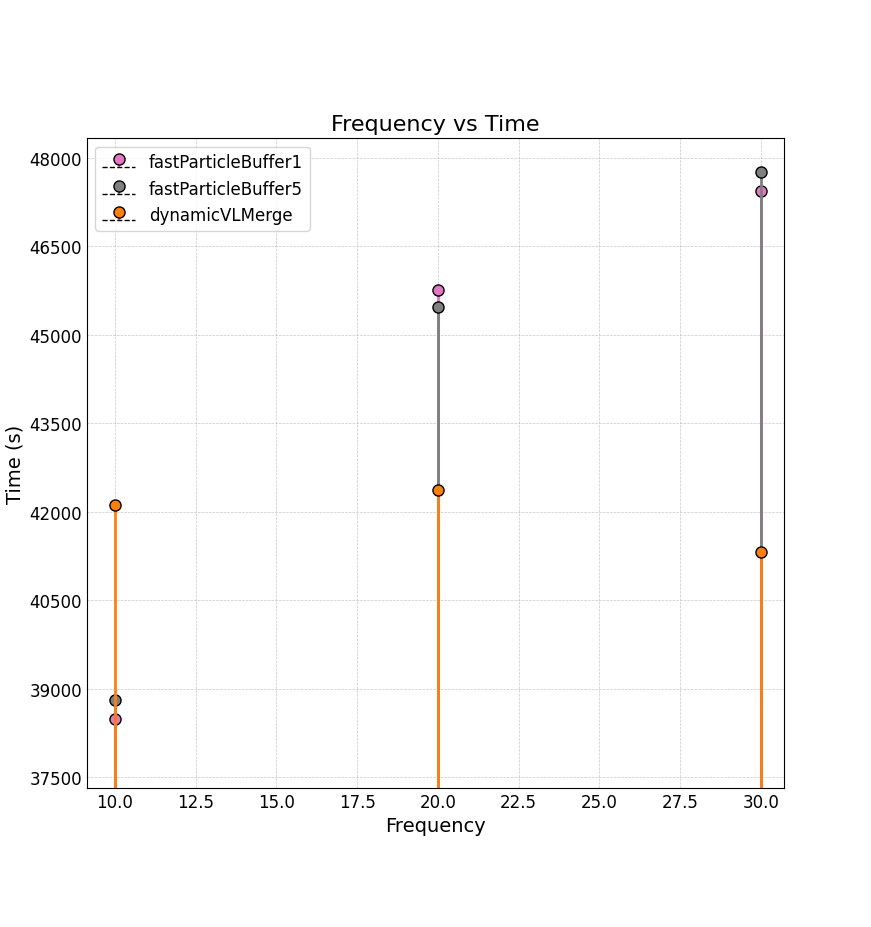
\includegraphics[width=0.6\linewidth]{graphs/spinodalDecomposition/vlcc08_increased.png}
\captionof{figure}{Iterations vs Time for Equilibration vlc\_c08 [\textbf{CHANGE GRAPH: include newer frequencies}]}
\end{center}


\section{Checkpoint Experiments}

\section{Hardware differences}



%%% -----------2 - 3 pages ---------------
\chapter{Future Work}

While the Fast-Particle-Buffer showed potential in larger simulations, it did not provide a significant performance improvement in smaller ones. Further research can focus on different aspects to enhance its efficiency.

One possible direction is studying how different hardware setups affect the buffer's performance. Running tests on various processors and memory architectures could help understand whether certain hardware configurations benefit more from the buffer approach.

Another improvement could involve combining the Fast-Particle-Buffer with Gall's adaptive neighbor list rebuild strategy. Since both methods aim to reduce the cost of rebuilding neighbor lists, merging them could lead to better overall performance.


Additionally, an alternative approach to identifying fast particles could be explored. Instead of classifying each particle individually, a group-based approach could be tested. The current definition of fast particles is based on how much a particle moves relative to its previous position, determining whether it has potentially left or entered another particle's search region. However, this classification does not consider relative motion within a larger system of particles.

If a group of particles moves as a unit, their positions relative to one another remain unchanged, meaning that no particle has actually moved into or out of another's search region. In this case, classifying them as fast particles and adding them to the buffer would be unnecessary because their relative interactions have not changed. By incorporating a group motion detection method, the buffer mechanism could avoid unnecessary classifications of fast particles, reducing remainder traversal costs. 


Testing the buffer in other larger and longer-running simulations could also be beneficial. While small simulations showed only minor improvements, a 6\% performance boost was observed in one of the longer simulations. This suggests that the effectiveness of the buffer may become more apparent in extended simulations. Running additional tests on different long-running scenarios could help determine whether if even greater performance gains can be achieved.

Finally, optimizing how buffer traversal is handled could further reduce remainder traversal time. Since remainder traversal is currently a major performance bottleneck, improving its efficiency could reveal the full advantages of the buffer approach.


\chapter{Conclusion}
This thesis investigated the Fast-Particle-Buffer as a method to reduce the computational cost of frequent neighbor list rebuilds in AutoPas. The approach aimed to improve simulation efficiency by temporarily storing fast particles instead of immediately rebuilding neighbor lists.  

Through a series of experiments, the performance of the buffer was evaluated under different scenarios, thresholds, and frequencies. The results showed that while the buffer did not significantly improve performance in smaller simulations, it provided measurable benefits in longer-running simulations, with a maximum observed speedup of 6\%.  

Further analysis revealed that remainder traversal time remained a key limiting factor, often negating the benefits of reduced neighbor list rebuilds. Additionally, the effectiveness of the buffer depended on the characteristics of the simulation.

Future work could explore hardware-dependent optimizations, integrating adaptive rebuild criteria, and exploring group-based fast particle classification. Additionally, optimizing buffer traversal could further reduce remainder traversal overhead, making the approach more performative.  

Overall, while the Fast-Particle-Buffer presents a good strategy for improving simulation performance, its benefits are highly scenario-dependent. With further refinements, it could become a useful optimization technique in AutoPas.



\appendix
\chapter{Appendix} \label{sec:appendix}
\section{}

% ================== Freq vs Time =====================
\begin{figure}[htbp]
    \centering
    \vspace{-0.5em}
    \begin{subfigure}[b]{\textwidth}
        \centering
        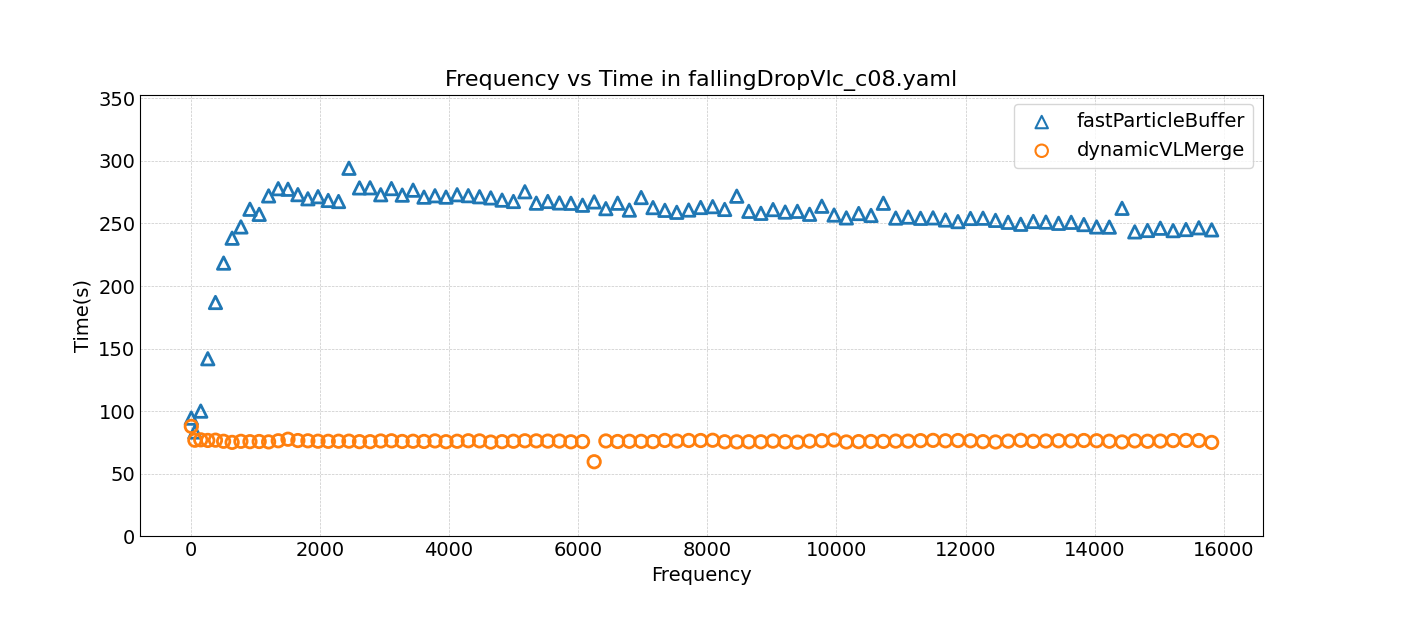
\includegraphics[width=0.9\linewidth]{graphs/fallingDrop/normalExperiments/freq/vlcc08.png}
        \vspace{-0.5em}
        \caption{\scriptsize Falling Drop vlc\_c08}
        \label{fig:vlcc08fallingDrop}
    \end{subfigure}

    \begin{subfigure}[b]{\textwidth}
        \centering
        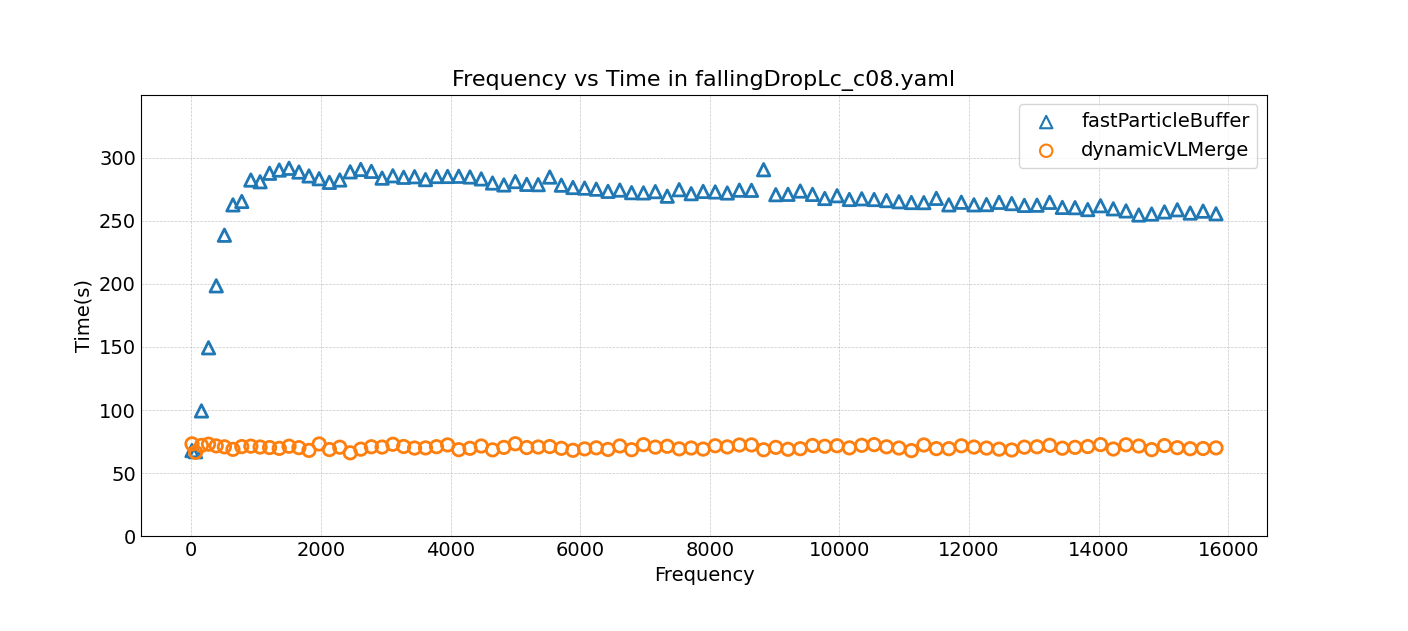
\includegraphics[width=0.9\linewidth]{graphs/fallingDrop/normalExperiments/freq/lcc08.png}
        \vspace{-0.5em}
        \caption{\scriptsize Falling Drop lc\_c08}
        \label{fig:lcc08explodingLiquid}
    \end{subfigure}

    \begin{subfigure}[b]{\textwidth}
        \centering
        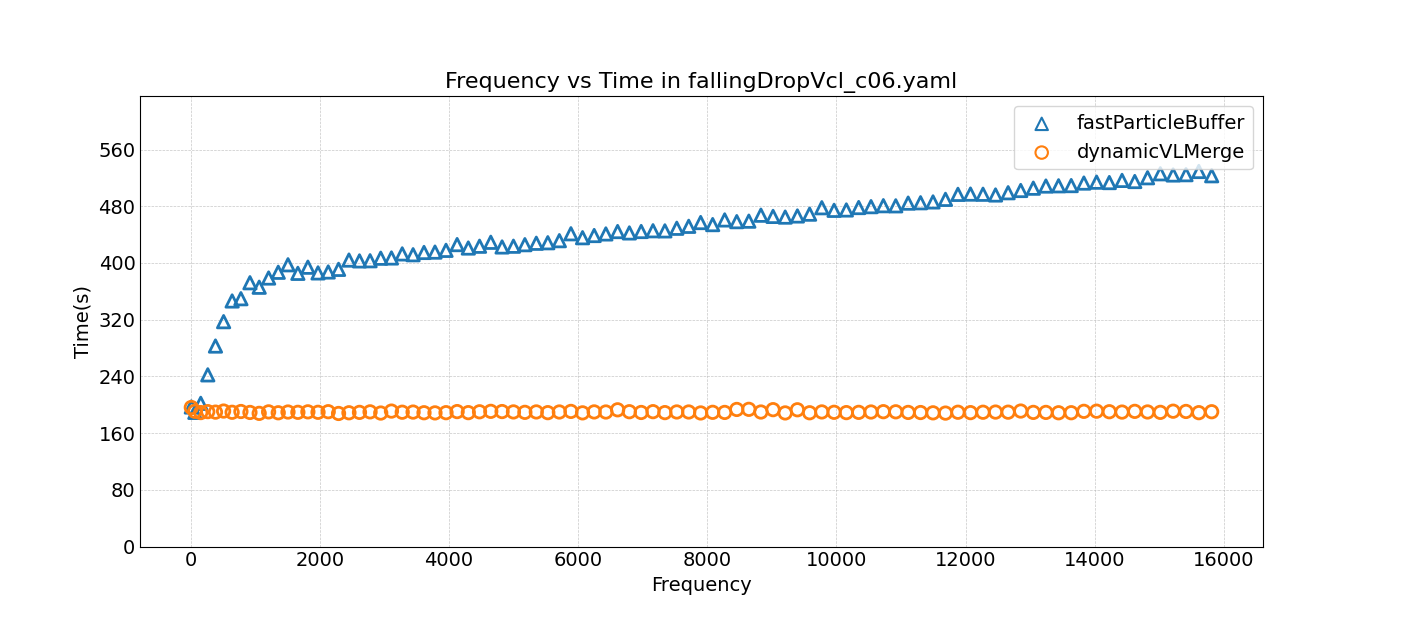
\includegraphics[width=0.9\linewidth]{graphs/fallingDrop/normalExperiments/freq/vclc06.png}
        \vspace{-0.5em}
        \caption{\scriptsize Falling Drop vcl\_c06}
        \label{fig:vclc06constantVelocityCube}
    \end{subfigure}

    \vspace{1em}
    \caption{Comparison of Frequency vs Time for Falling Drop Experiments}
    \label{fig:mainFallingDrop}
\end{figure}


\begin{figure}[htbp]
    \centering
    \vspace{-0.5em}
    \begin{subfigure}[b]{\textwidth}
        \centering
        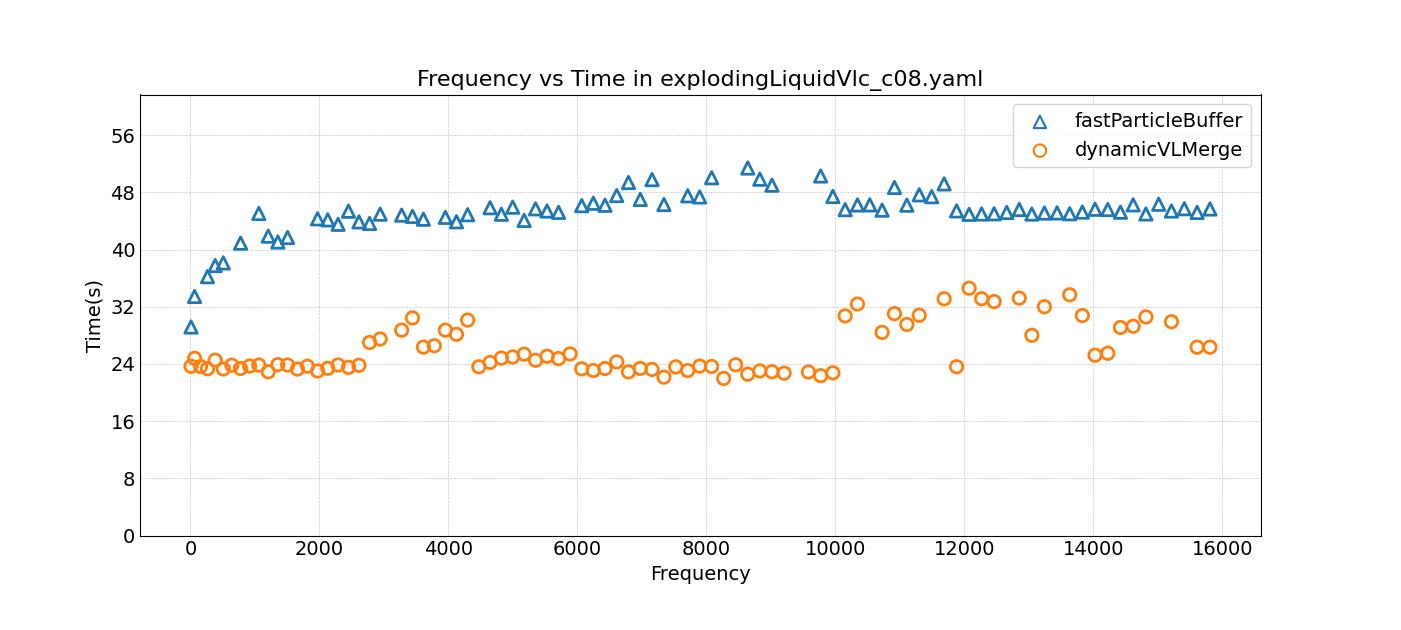
\includegraphics[width=0.9\linewidth]{graphs/explodingLiquid/normalExperiments/freq/vlcc08.png}
        \vspace{-0.5em}
        \caption{\scriptsize Exploding Liquid vlc\_c08}
        \label{fig:vlcc08explodingLiquid}
    \end{subfigure}

    \begin{subfigure}[b]{\textwidth}
        \centering
        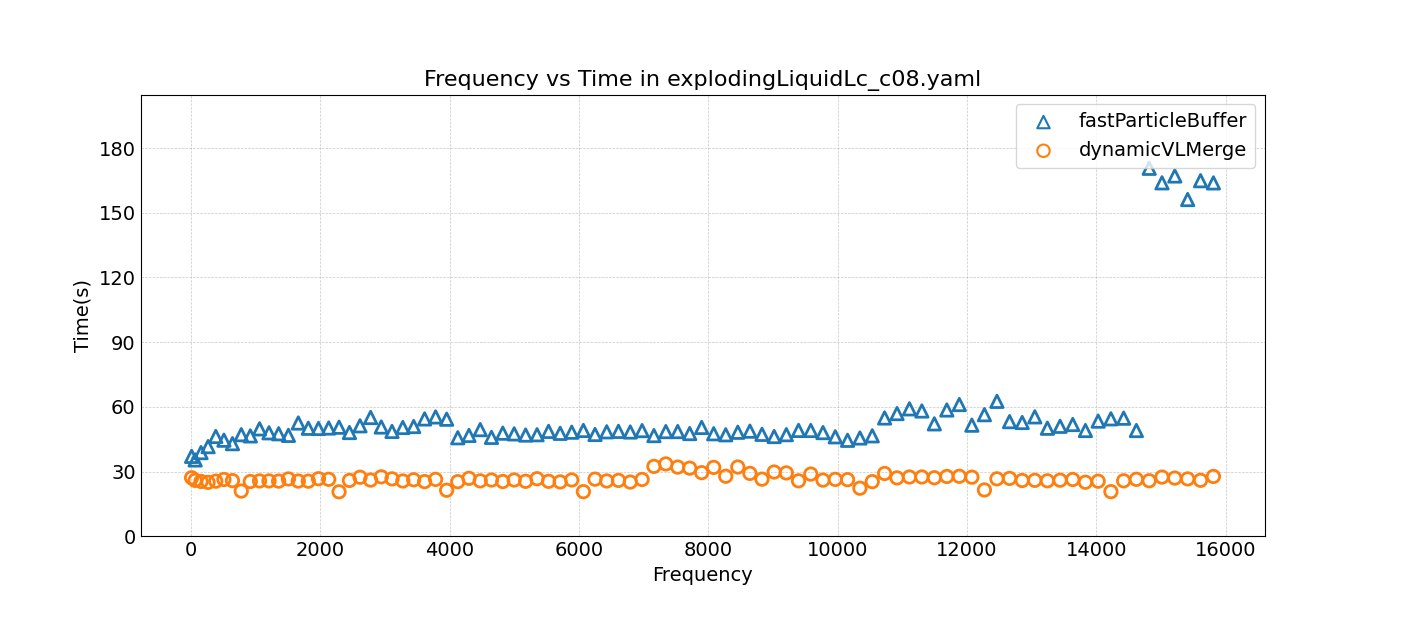
\includegraphics[width=0.9\linewidth]{graphs/explodingLiquid/normalExperiments/freq/lcc08.png}
        \vspace{-0.5em}
        \caption{\scriptsize Exploding Liquid lc\_c08}
        \label{fig:lcc08explodingLiquid}
    \end{subfigure}

    \begin{subfigure}[b]{\textwidth}
        \centering
        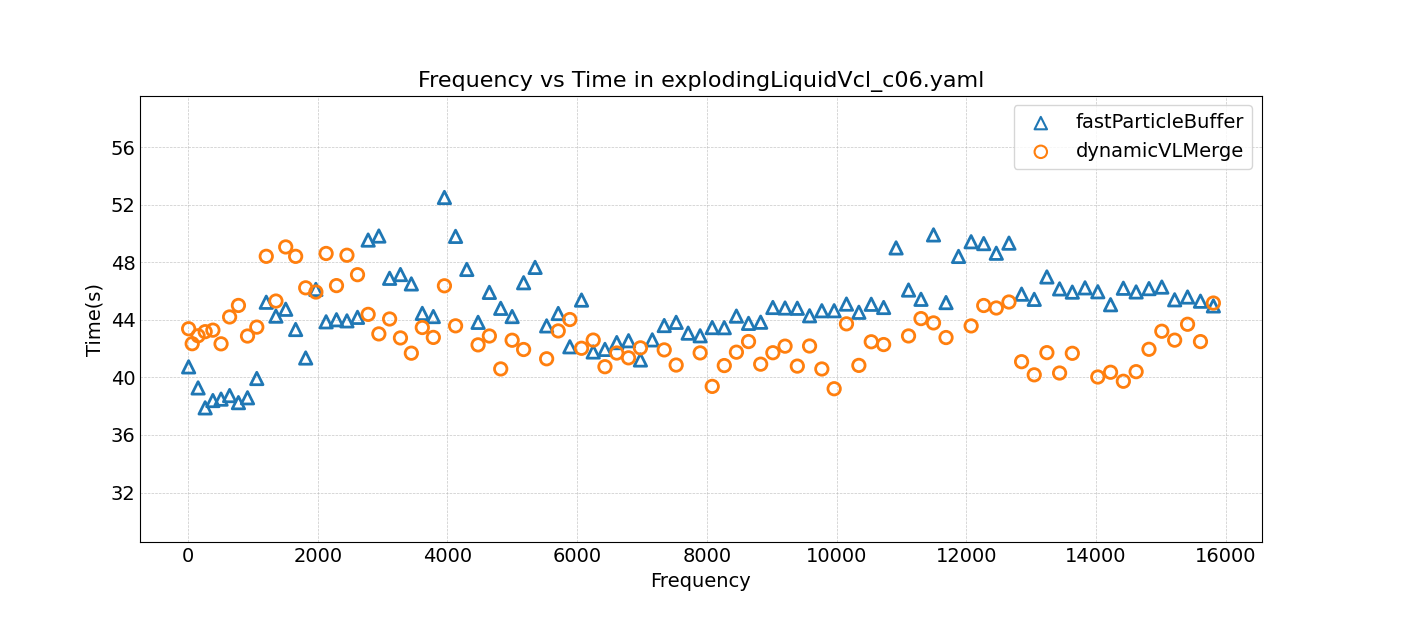
\includegraphics[width=0.9\linewidth]{graphs/explodingLiquid/normalExperiments/freq/vclc06.png}
        \vspace{-0.5em}
        \caption{\scriptsize Exploding Liquid vcl\_c06}
        \label{fig:vclc06explodingLiquid}
    \end{subfigure}

    \vspace{1em}
    \caption{Comparison of Frequency vs Time for Exploding Liquid Experiments}
    \label{fig:mainExplodingLiquid}
\end{figure}


\begin{figure}[htbp]
    \centering
    \vspace{-0.5em}
    \begin{subfigure}[b]{\textwidth}
        \centering
        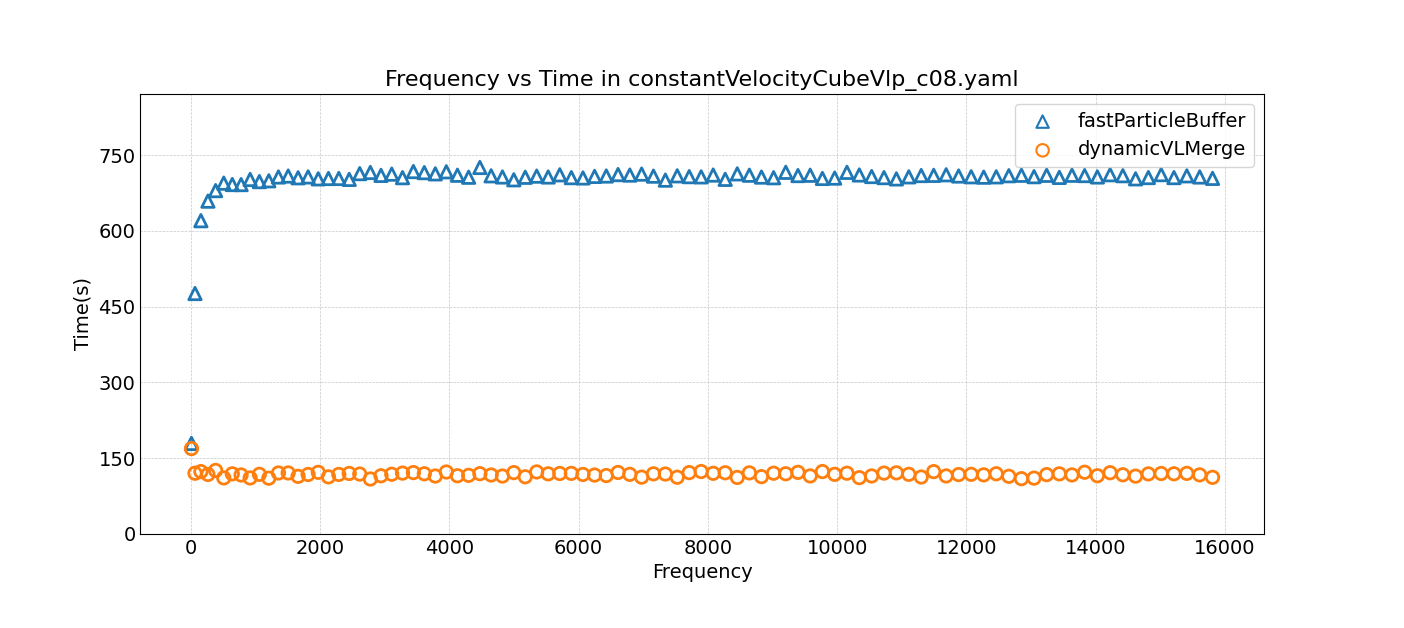
\includegraphics[width=0.9\linewidth]{graphs/constantVelocityCube/normalExperiments/freq/vlpc08.png}
        \vspace{-0.5em}
        \caption{\scriptsize Constant Velocity Cube vlp\_c08}
        \label{fig:vlpc08constantVelocityCube}
    \end{subfigure}

    \begin{subfigure}[b]{\textwidth}
        \centering
        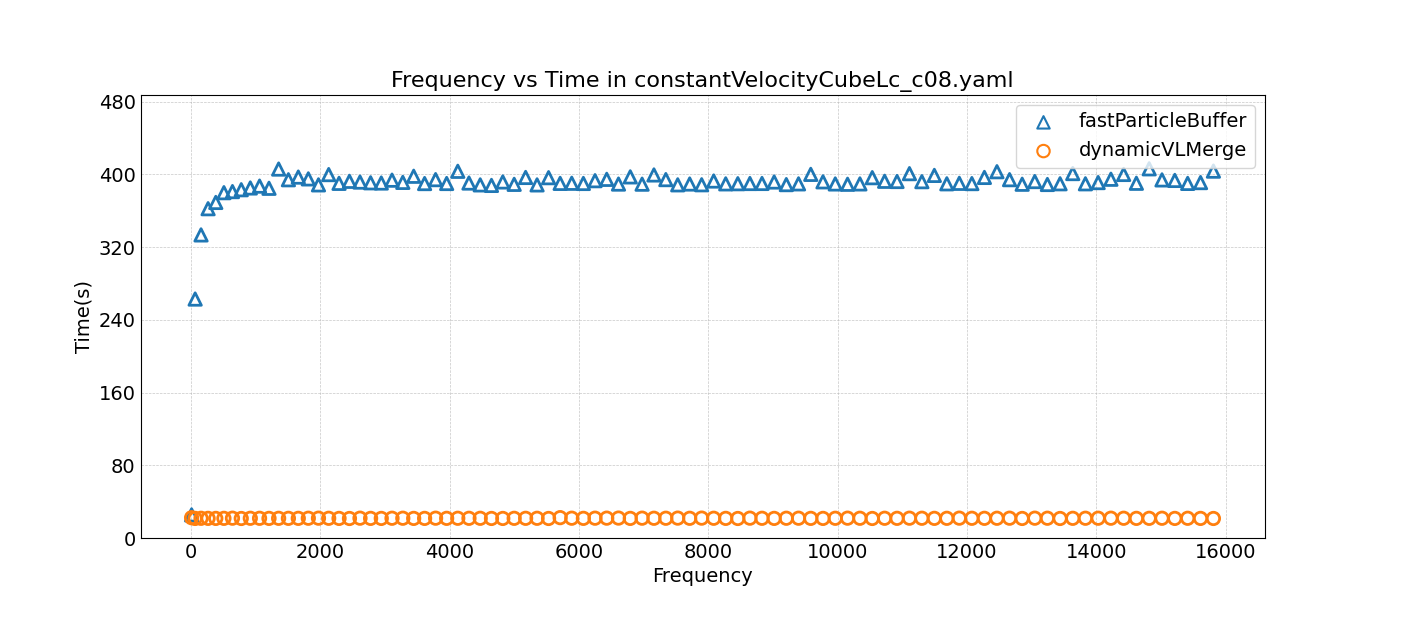
\includegraphics[width=0.9\linewidth]{graphs/constantVelocityCube/normalExperiments/freq/lcc08.png}
        \vspace{-0.5em}
        \caption{\scriptsize Constant Velocity Cube lc\_c08}
        \label{fig:lcc08constantVelocityCube}
    \end{subfigure}

    \begin{subfigure}[b]{\textwidth}
        \centering
        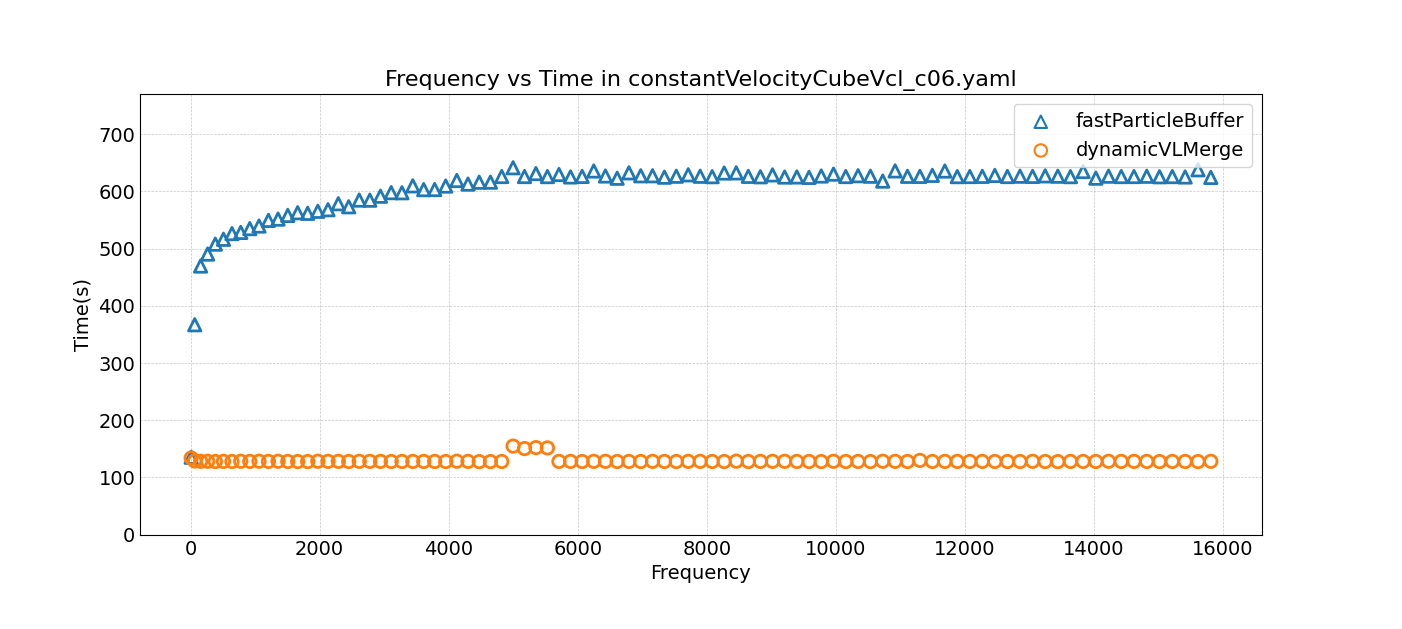
\includegraphics[width=0.9\linewidth]{graphs/constantVelocityCube/normalExperiments/freq/vclc06.png}
        \vspace{-0.5em}
        \caption{\scriptsize Constant Velocity Cube vcl\_c06}
        \label{fig:vclc06constantVelocityCube}
    \end{subfigure}

    \vspace{1em}
    \caption{Comparison of Frequency vs Time for Constant Velocity Cube Experiments}
    \label{fig:mainConstantVelocityCube}
\end{figure}

% ======================================================


% =====================Compute Inter vs Remainder Traversal Exploding Liquid=================================

\begin{figure}[htbp]
    \centering
    \vspace{-0.5em}
    \begin{subfigure}[b]{\textwidth}
        \centering
        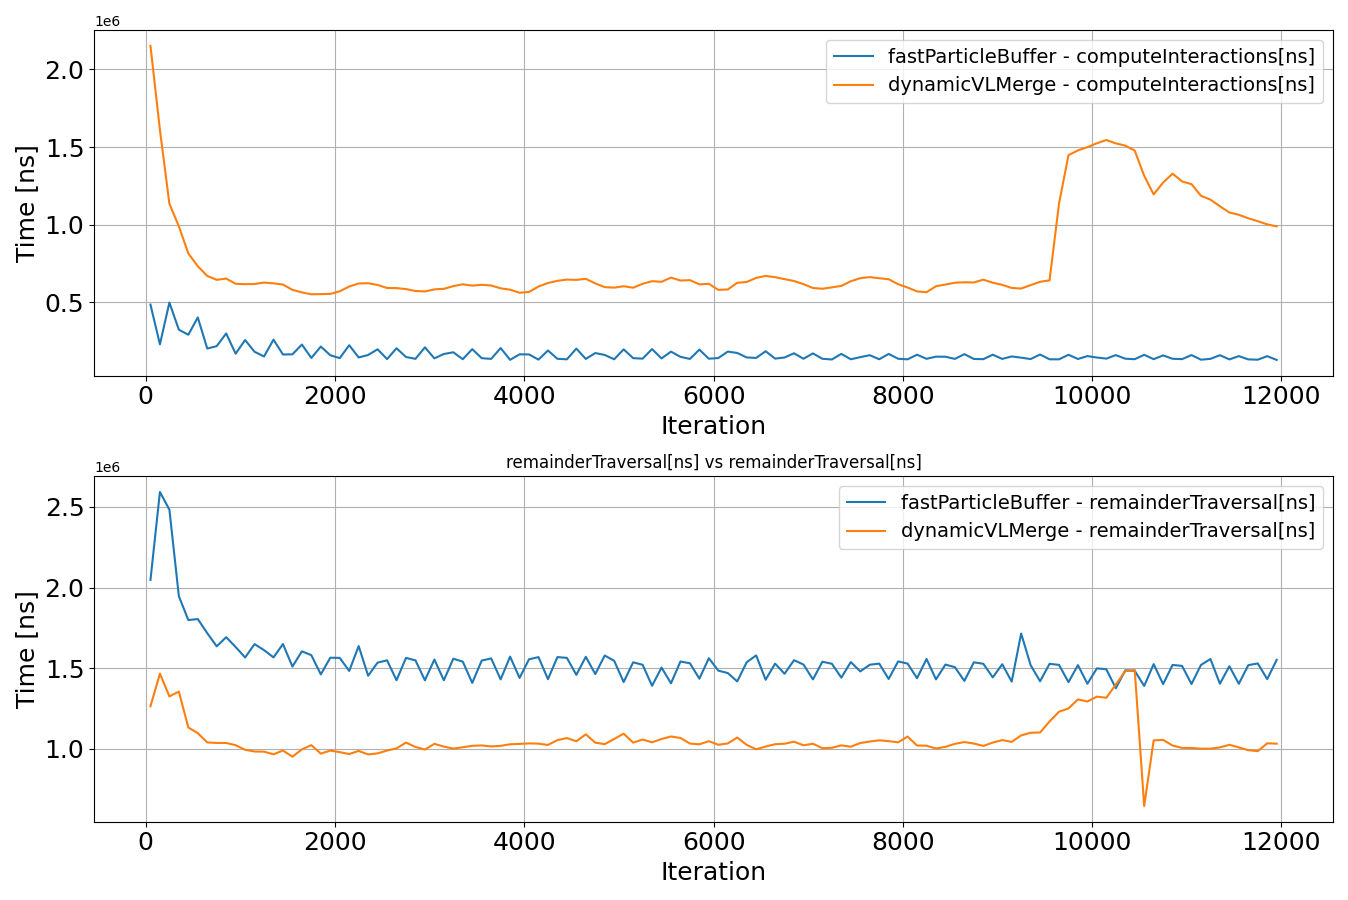
\includegraphics[width=0.9\linewidth]{graphs/explodingLiquid/normalExperiments/freq/vclc0_6inter.png}
        \vspace{-0.5em}
        \caption{\scriptsize Exploding Liquid Vcl\_c06}
        \label{fig:explodingLiquid_vclc0_6inter}
    \end{subfigure}

    \begin{subfigure}[b]{\textwidth}
        \centering
        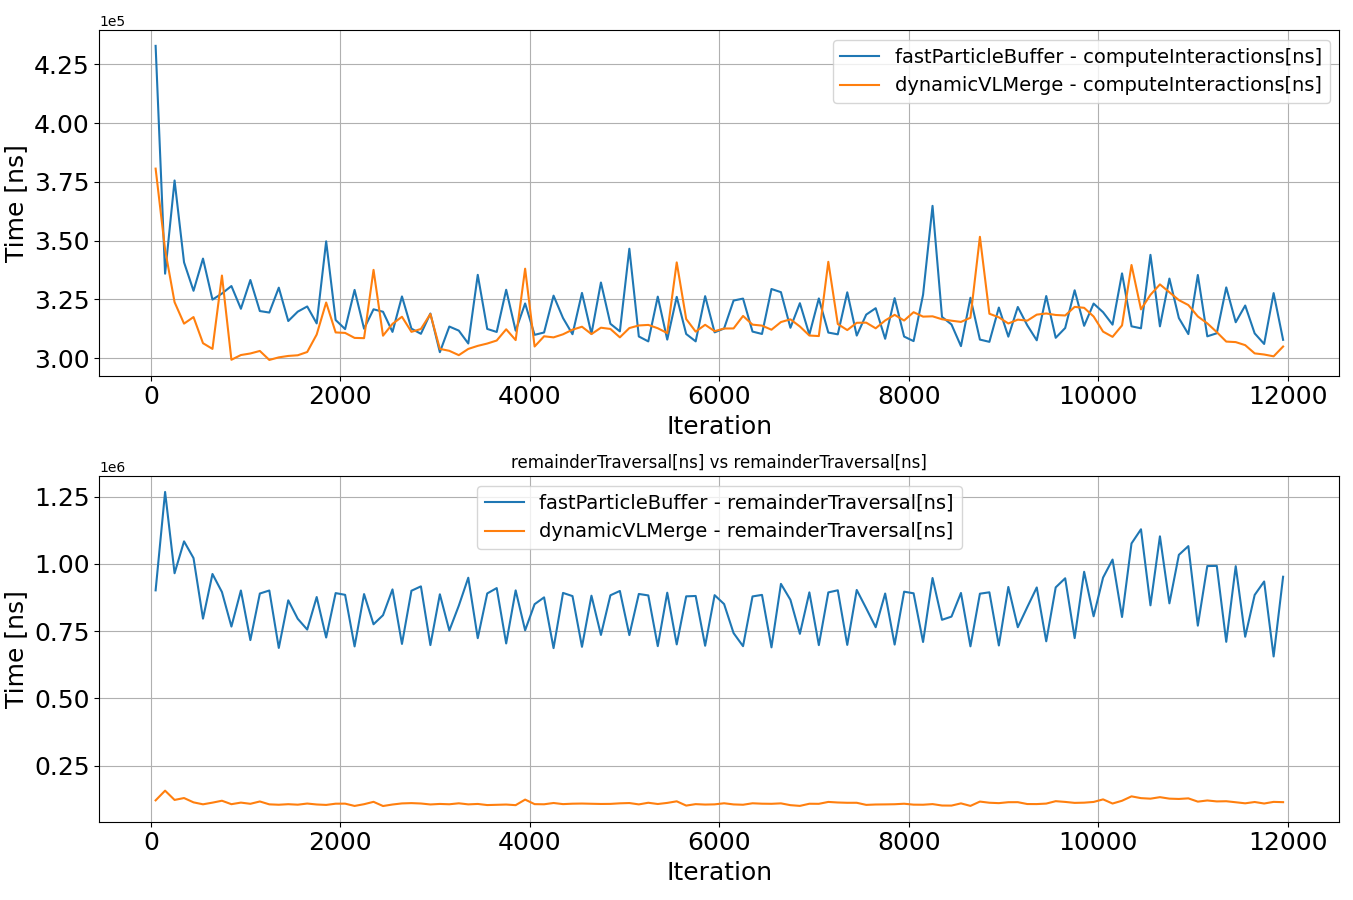
\includegraphics[width=0.9\linewidth]{graphs/explodingLiquid/normalExperiments/freq/vlc_c08inter.png}
        \vspace{-0.5em}
        \caption{\scriptsize Exploding Liquid Vlc\_c08}
        \label{fig:explodingLiquid_vlc_c08inter}
    \end{subfigure}

    \vspace{1em}
    \caption{Comparison of Compute Interactions and Remainder Traversal for Exploding Liquid Experiments}
    \label{fig:mainexplodingLiquid_inter}
\end{figure}
% ======================================================

% ============================== Iteration vs Time ==============================
\section{}
\begin{figure}[H]
\centering
% Subfigure 1
\begin{subfigure}{\linewidth}
    \centering
    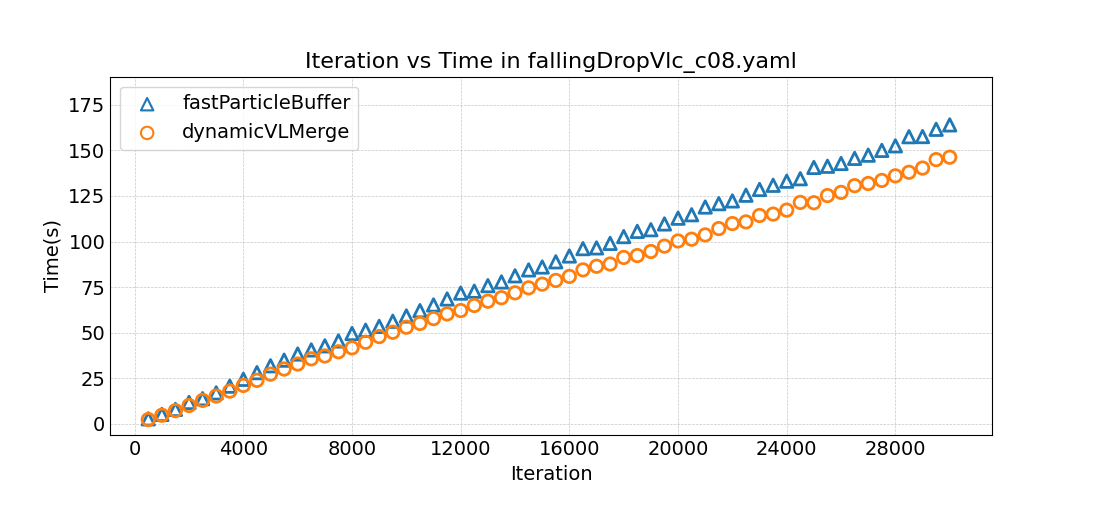
\includegraphics[width=\linewidth]{graphs/fallingDrop/normalExperiments/iter/vlcc08.png}
    \caption{Iterations vs Time for Falling Drop vlc\_c08}
    \label{fig:fallingDrop}
\end{subfigure}

% Subfigure 2
\begin{subfigure}{\linewidth}
    \centering
    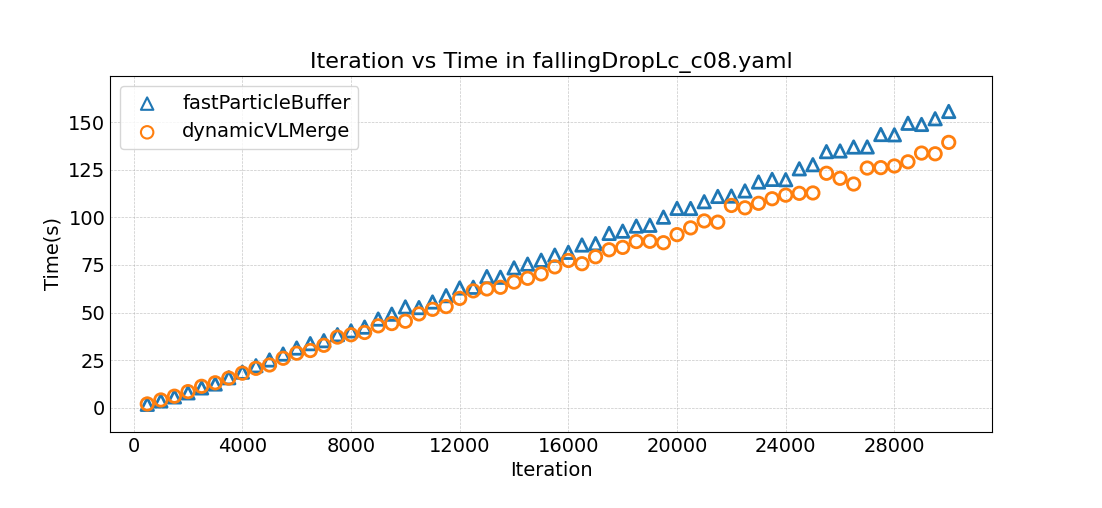
\includegraphics[width=\linewidth]{graphs/fallingDrop/normalExperiments/iter/lcc08.png}
    \caption{Iterations vs Time for Falling Drop lc\_c08}
    \label{fig:explodingLiquid}
\end{subfigure}

\label{fig:appendixGraphs}
\end{figure}

\begin{figure}[H]\ContinuedFloat
\centering
% Subfigure 3
\begin{subfigure}{\linewidth}
    \centering
    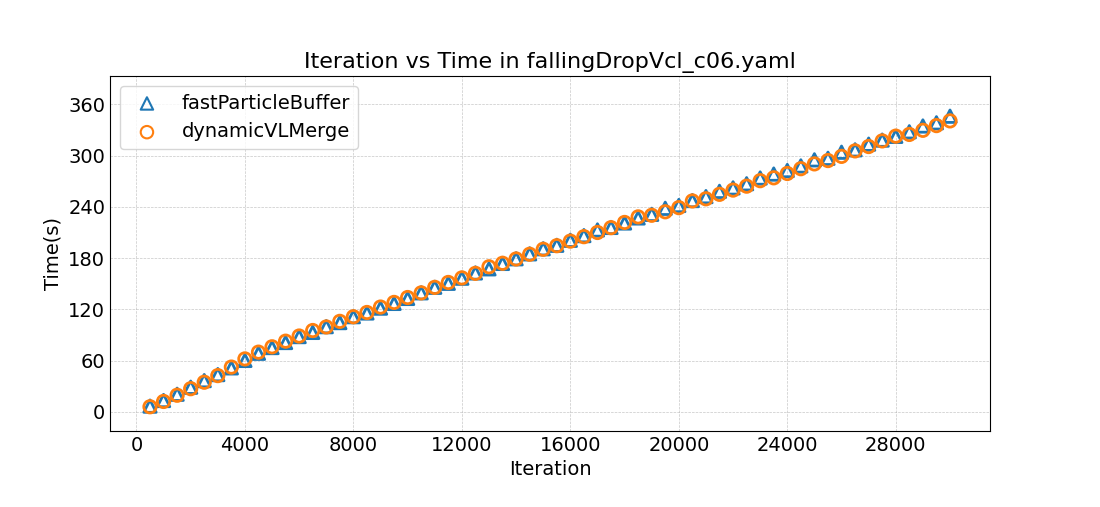
\includegraphics[width=\linewidth]{graphs/fallingDrop/normalExperiments/iter/vclc06.png}
    \caption{Iterations vs Time for Falling Drop vcl\_c06}
    \label{fig:constantVelocityCube}
\end{subfigure}
\end{figure}

\section{}
\begin{figure}[H]
\centering
% Subfigure 1
\begin{subfigure}{\linewidth}
    \centering
    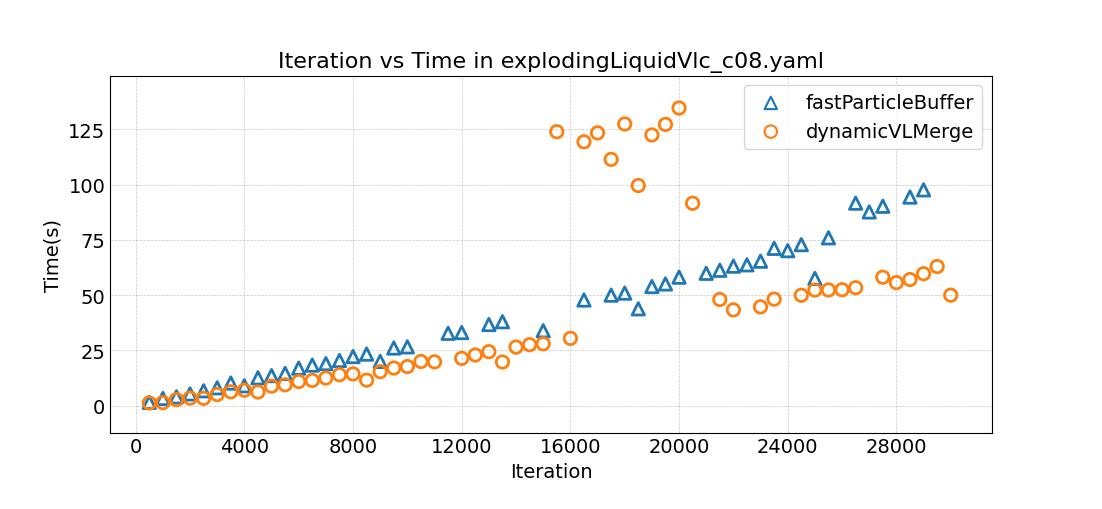
\includegraphics[width=\linewidth]{graphs/explodingLiquid/normalExperiments/iter/vlcc08.png}
    \caption{Iterations vs Time for Exploding Liquid vlc\_c08}
    \label{fig:fallingDrop}
\end{subfigure}

% Subfigure 2
\begin{subfigure}{\linewidth}
    \centering
    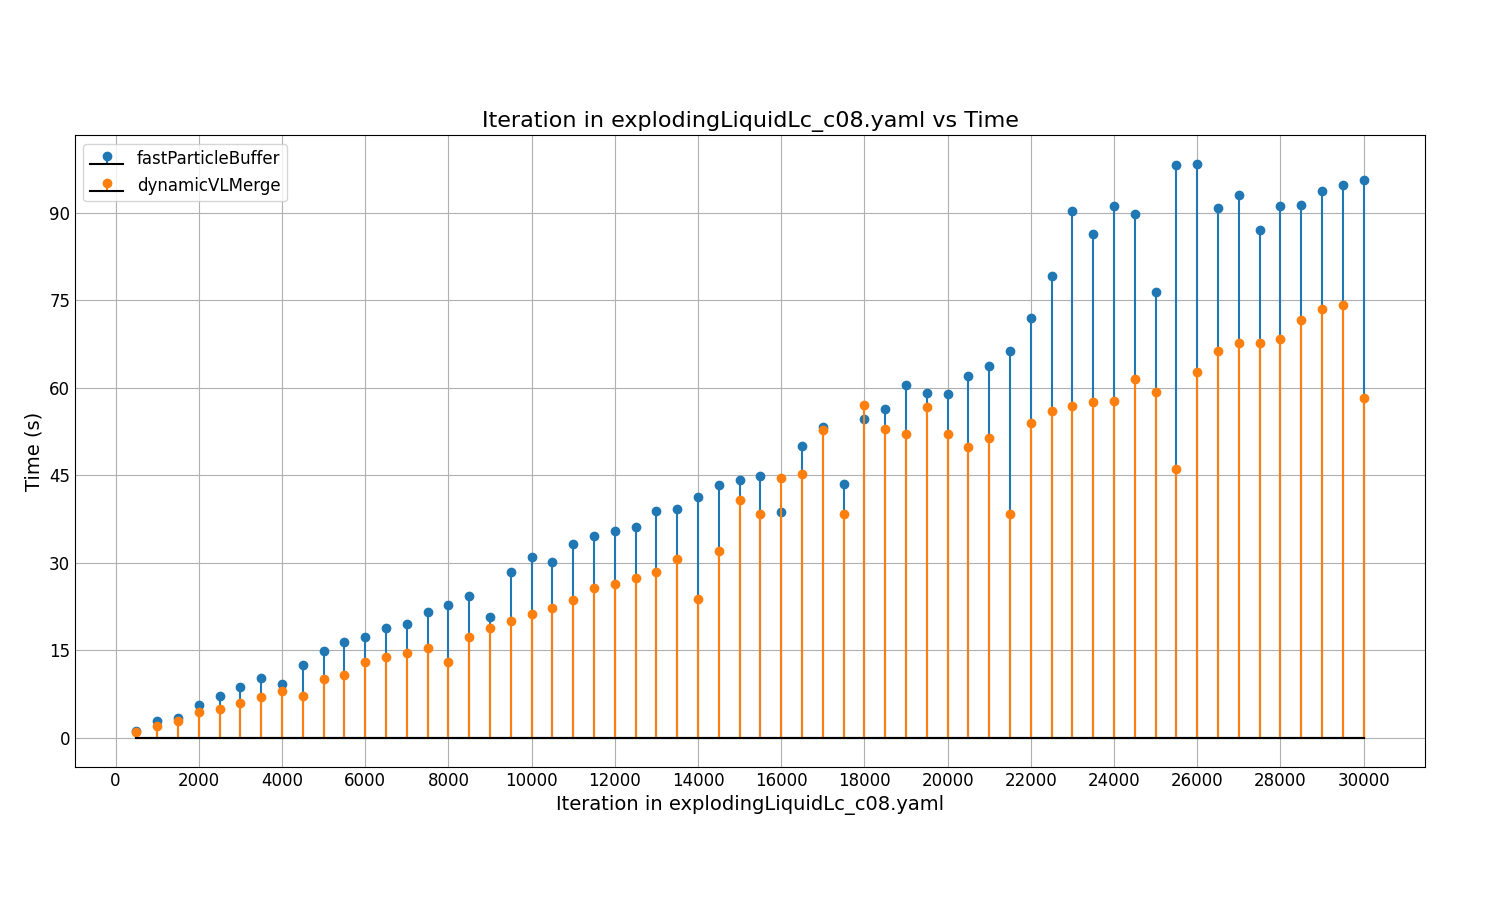
\includegraphics[width=\linewidth]{graphs/explodingLiquid/normalExperiments/iter/lcc08.png}
    \caption{Iterations vs Time for Exploding Liquid lc\_c08}
    \label{fig:explodingLiquid}
\end{subfigure}

\label{fig:appendixGraphs}
\end{figure}

\begin{figure}[H]\ContinuedFloat
\centering
% Subfigure 3
\begin{subfigure}{\linewidth}
    \centering
    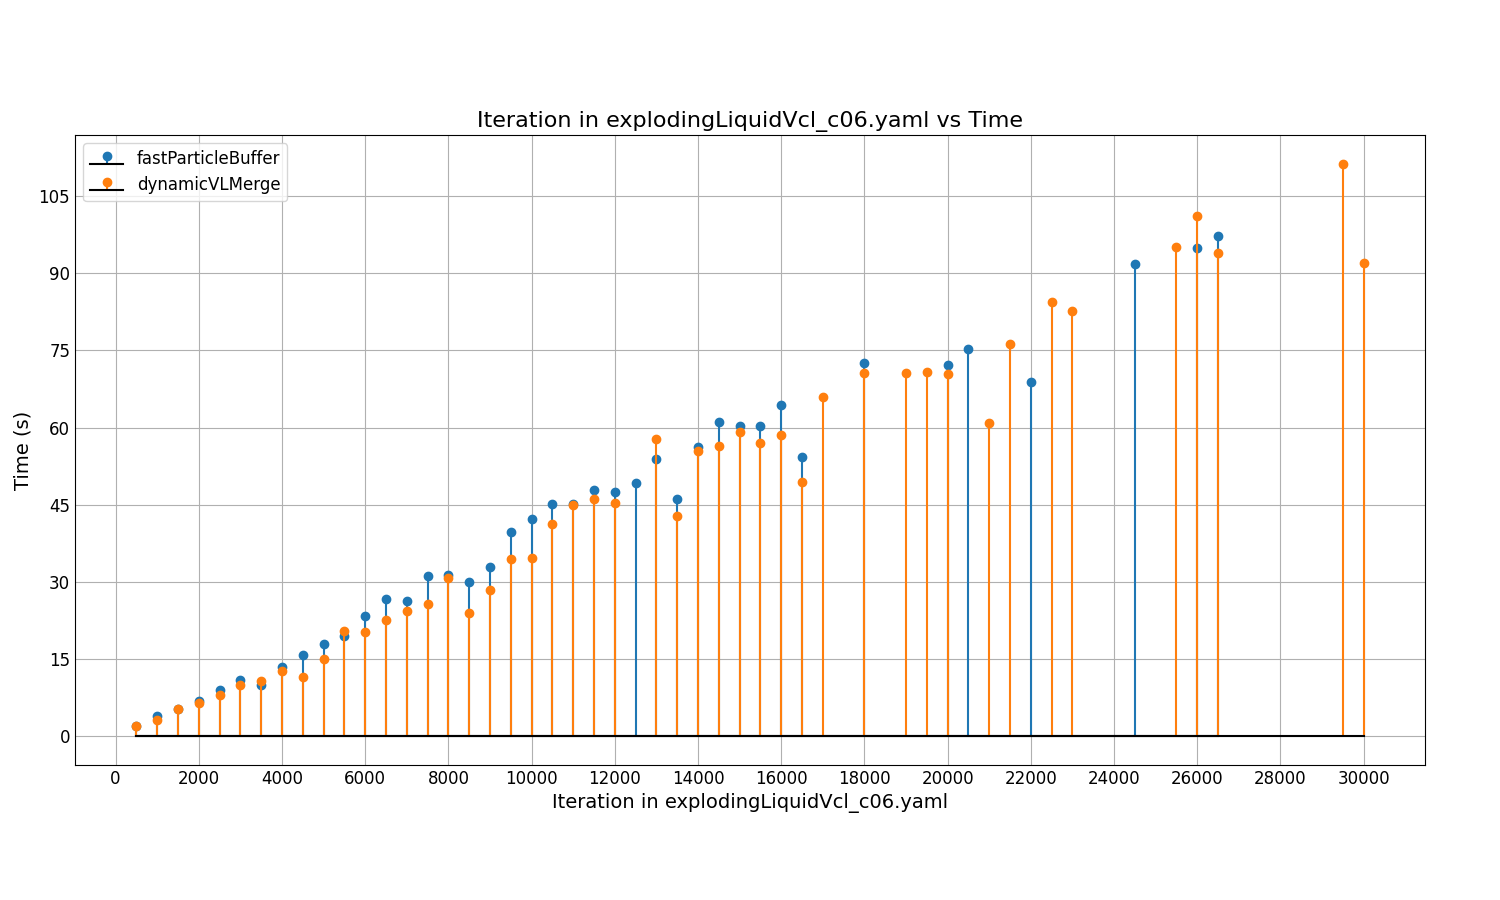
\includegraphics[width=\linewidth]{graphs/explodingLiquid/normalExperiments/iter/vclc06.png}
    \caption{Iterations vs Time for Exploding Liquid vcl\_c06}
    \label{fig:constantVelocityCube}
\end{subfigure}
\end{figure}

\section{}
\begin{figure}[H]
\centering
% Subfigure 1
\begin{subfigure}{\linewidth}
    \centering
    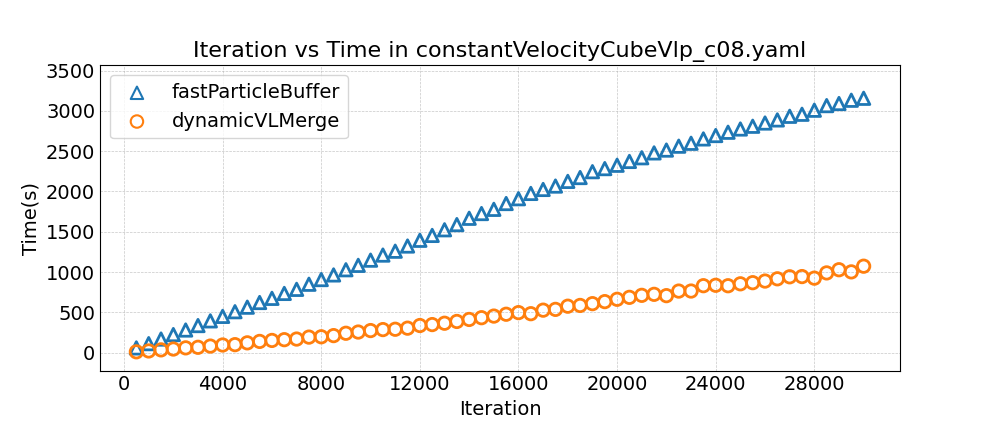
\includegraphics[width=\linewidth]{graphs/constantVelocityCube/normalExperiments/iter/vlpc08.png}
    \caption{Iterations vs Time for Constant Velocity Cube vlp\_c08}
    \label{fig:fallingDrop}
\end{subfigure}

% Subfigure 2
\begin{subfigure}{\linewidth}
    \centering
    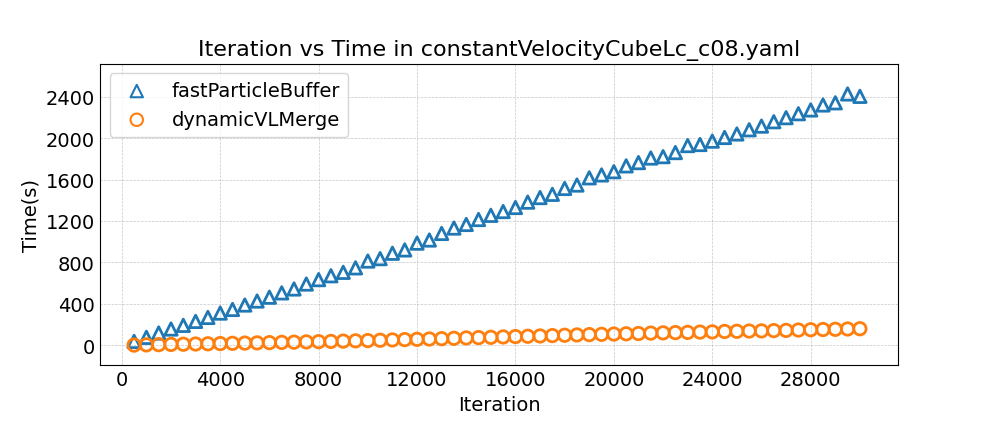
\includegraphics[width=\linewidth]{graphs/constantVelocityCube/normalExperiments/iter/lcc08.png}
    \caption{Iterations vs Time for Constant Velocity Cube lc\_c08}
    \label{fig:explodingLiquid}
\end{subfigure}

\label{fig:appendixGraphs}
\end{figure}

\begin{figure}[H]\ContinuedFloat
\centering
% Subfigure 3
\begin{subfigure}{\linewidth}
    \centering
    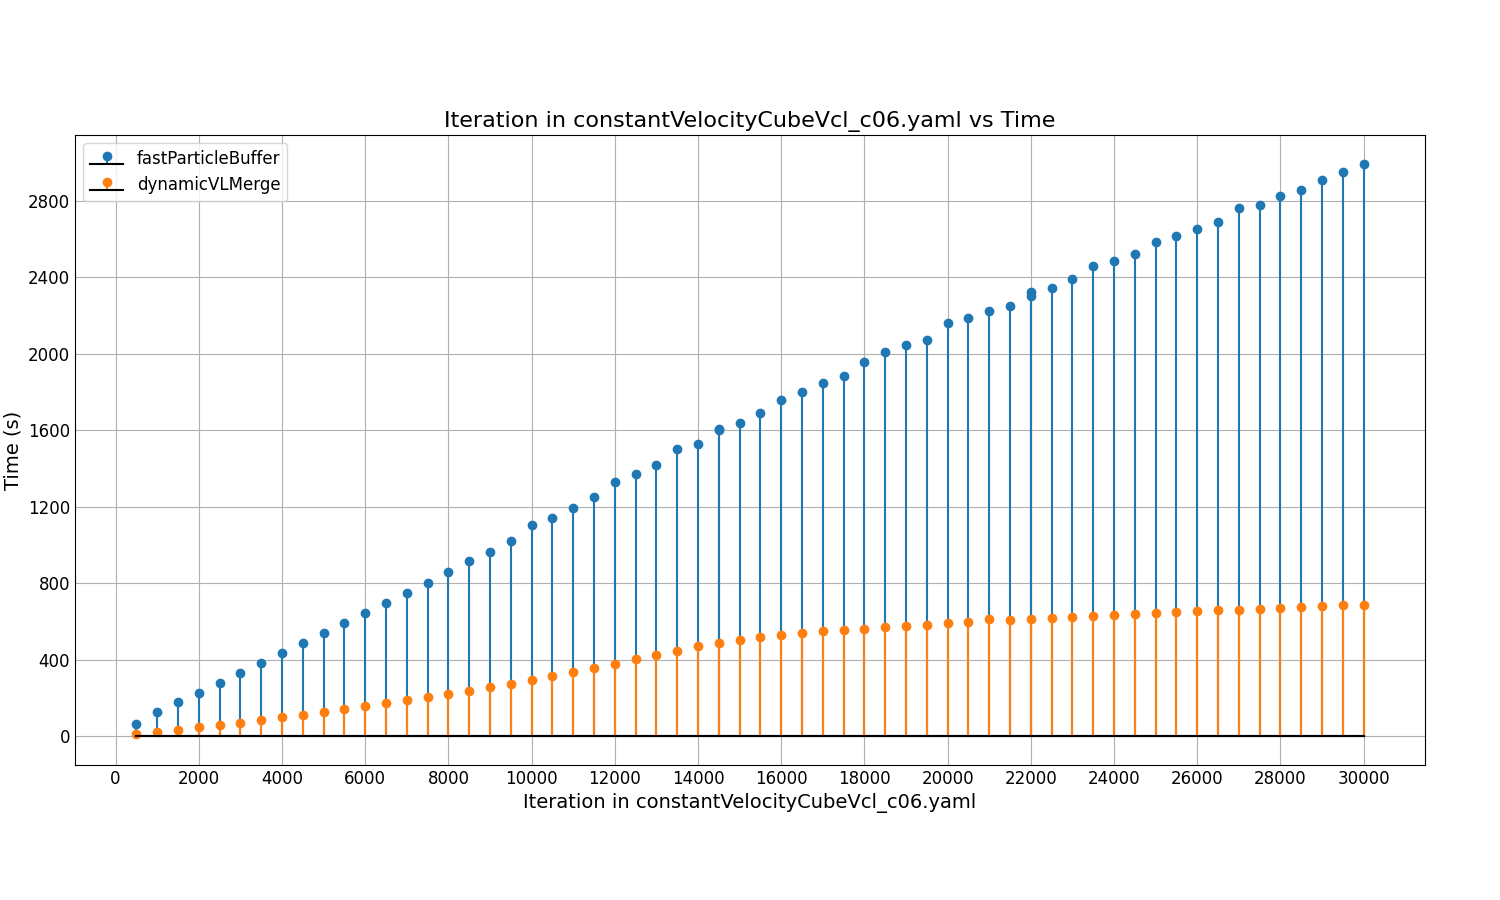
\includegraphics[width=\linewidth]{graphs/constantVelocityCube/normalExperiments/iter/vclc06.png}
    \caption{Iterations vs Time for Constant Velocity Cube vcl\_c06}
    \label{fig:constantVelocityCube}
\end{subfigure}
\end{figure}



% ======================================================



% ==================Spinodal Decomposition Equilibration ====================

\section{}
\begin{figure}[H]
\centering
% Subfigure 1
\begin{subfigure}{\linewidth}
    \centering
    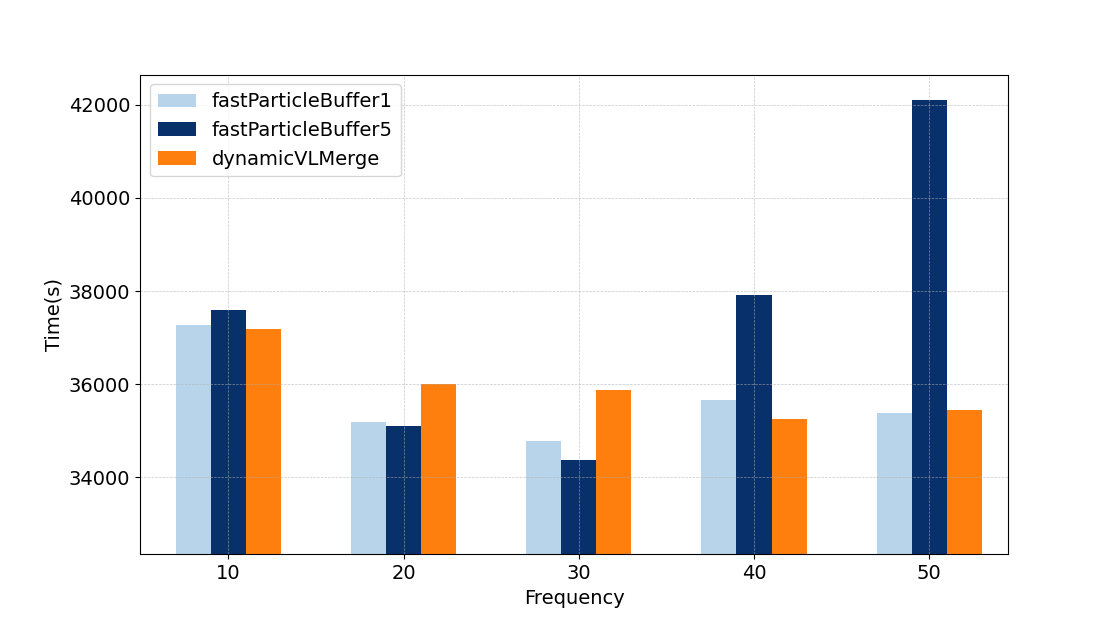
\includegraphics[width=\linewidth]{graphs/spinodalDecomposition/vlcc08.png}
    \caption{Iterations vs Time for Spinodal Decomposition vlc\_c08}
    \label{fig:fallingDrop}
\end{subfigure}

% Subfigure 2
\begin{subfigure}{\linewidth}
    \centering
    \includegraphics[width=\linewidth]{graphs/spinodalDecomposition/lcc08.png}
    \caption{Frequency vs Time for Spinodal Decomposition lc\_c08}
    \label{fig:explodingLiquid}
\end{subfigure}

\label{fig:appendixGraphs}
\end{figure}

% ======================================================



\appendix{}




\microtypesetup{protrusion=false}
\listoffigures{}
\listoftables{}
\microtypesetup{protrusion=true}
\printbibliography{}

\end{document}
